%%%% Time-stamp: <2018-03-24 14:05:09 vk>
%% ========================================================================
%%%% Disclaimer
%% ========================================================================
%%
%% created by
%%
%%      Karl Voit
%%

%% ========================================================================
%%%% Basic settings
%% ========================================================================
%% (idea of using newcommands for basic documentclass settings from: Thomas Schlager)

\newcommand{\mypapersize}{A4}
%% e.g., "A4", "letter", "legal", "executive", ...
%% The size of the paper of the resulting PDF file.

\newcommand{\mylaterality}{twoside}
%% "oneside" or "twoside"
%% Either you are creating a document which is printed on both, left pages
%% and right pages (twoside) or you create a document which is printed
%% on right pages only (oneside).

\newcommand{\mydraft}{false}
%% "true" or "false"
%% Use draft mode? If true, included graphics are replaced by empty
%% rectangles (of same size) and overfull boxes (in margin space) are
%% marked with black box (-> easy to spot!)

\newcommand{\myparskip}{half}
%% e.g., "no", "full", "half", ...
%% How to separate paragraphs: indention ("no") or spacing ("half",
%% "full", ...).

\newcommand{\myBCOR}{0mm}
%% Inner binding correction. This value depends on the method which is
%% being used to bind your printed result. Some techniques do not
%% require a binding correction at all ("0mm"), other require for
%% example "5mm". Refer to KOMA script documentation for a detailed
%% explanation what a binding correction is and how to measure it.

\newcommand{\myfontsize}{12pt}
%% e.g., 10pt, 11pt, 12pt
%% The font size of the main text in pt (points).

\newcommand{\mylinespread}{1.0}
%% e.g., 1.0, 1.5, 2.0
%% Line spacing in %/100. For example 1.5 means 150% of the usual line
%% spacing. Please use with caution: 100% ("1.0") is fine because the
%% font was designed for it.

\newcommand{\mylanguage}{ngerman,american}
%% "english,ngerman", "ngerman,english", ...
%% NOTE: The *last* language is the active one!
%% See babel documentation for further details.

%% BibLaTeX-settings: (see biblatex reference for further description)
\newcommand{\mybiblatexstyle}{authoryear}

%% e.g., "alphabetic", "authoryear", ...
%% The biblatex style which is being used for referencing. See
%% biblatex documentation for further details and more values.
%%
%% CAUTION: if you change the style, please check for (in)compatible
%%          "biblatex" package options in the file
%%          "template/preamble.tex"! For example: "alphabetic" does
%%          not have an option "dashed=..." and causes an error if it
%%          does not get removed from the list of options.

\newcommand{\mybiblatexdashed}{false}  %% "true" or "false"
%% If true: replace recurring reference authors with a dash.

\newcommand{\mybiblatexbackref}{true}  %% "true" or "false"
%% If true: create backward links from reference to citations.

\newcommand{\mybiblatexfile}{references.bib}
%% Name of the biblatex file that holds the references.

\newcommand{\mydispositioncolor}{30,103,182}
%% e.g., "30,103,182" (blue/turquois), "0,0,0" (black), ...
%% Color of the headings and so forth in RGB (red,green,blue) values.
%% NOTE: if you are using "0,0,0" for black, printers might still
%%       recognize pages as color pages. In case this is a problem
%%       (paying for color print-outs vs. paying for b/w-printouts)
%%       please edit file "template/preamble.tex" and change
%%       "\definecolor{DispositionColor}{RGB}{\mydispositioncolor}"
%%       to "\definecolor{DispositionColor}{gray}{0}" and thus
%%       overwriting the value of \mydispositioncolor above.

\newcommand{\mycolorlinks}{true}  %% "true" or "false"
%% Enables or disables colored links (hyperref package).

\newcommand{\mytitlepage}{template/title_Thesis_UOC}
%% Your own or one of following pre-defined title pages:
%% "template/title_plain_maketitle": simple maketitle page
%% "template/title_Diplomarbeit_KF_Uni_Graz.tex": fancy (german) title page for KF Uni Graz
%% "template/title_Thesis_TU_Graz":
%%             titlepage for Graz University of Technology (correct
%%             (old?) Corporate Design) by Karl Voit (2012)
%% "template/title_Thesis_TU_Graz_-_kazemakase":
%%             titlepage for Graz University of Technology
%%             (correct new Corporate Design) by kazemakase (2013):
%%             see https://github.com/novoid/LaTeX-KOMA-template/issues/5
%% "template/title_VWA": titlepage for Vorwissenschaftliche Arbeit

\newcommand{\mytodonotesoptions}{}
%% e.g., "" (empty), "disable", ...
%% Options for the todonotes-package. If "disable", all todonotes will
%% be hidden (including listoftodos).

%% Load main settings for document preamble:
%% Time-stamp: <2018-03-11 14:25:47 vk>
%%%% === Disclaimer: =======================================================
%% created by
%%
%%      Karl Voit
%%
%% using GNU/Linux, GNU Emacs & LaTeX 2e
%%

%doc% %% overriding preamble/preamble.tex %%
%doc% \newcommand{\mylinespread}{1.0}  \newcommand{\mycolorlinks}{true}
%doc% \documentclass[12pt,paper=a4,parskip=half,DIV=calc,oneside,%%
%doc% headinclude,footinclude=false,open=right,bibliography=totoc]{scrartcl}
%doc% \usepackage[utf8]{inputenc}\usepackage[ngerman,american]{babel}\usepackage{scrpage2}
%doc% \usepackage{ifthen}\usepackage{eurosym}\usepackage{xspace}\usepackage[usenames,dvipsnames]{xcolor}
%doc% \usepackage[protrusion=true,factor=900]{microtype}
%doc% \usepackage{enumitem}
%doc% \usepackage[pdftex]{graphicx}
%doc% \usepackage{todonotes}
%doc% \usepackage{dingbat,bbding} %% special characters
%doc% \definecolor{DispositionColor}{RGB}{30,103,182}
%doc%
%doc% \usepackage[backend=biber,style=authoryear,dashed=false,natbib=true,hyperref=true%%
%doc% ]{biblatex}
%doc%
%doc% \addbibresource{references-biblatex.bib} %% remove, if using BibTeX instead of biblatex
%doc%
%doc% %% overriding userdata %%
%doc% \newcommand{\myauthor}{Karl Voit}\newcommand{\mytitle}{LaTeX Template Documentation}
%doc% \newcommand{\mysubject}{A Comprehensive Guide to Use the
%doc% Template from https://github.com/novoid/LaTeX-KOMA-template}
%doc% \newcommand{\mykeywords}{LaTeX, pdflatex, template, documentation, biber, biblatex}
%doc%
%doc% \newcommand{\myLaT}{\LaTeX{}@TUG\xspace}
%doc%
%doc% %% for future use?
%doc% % \usepackage{filecontents}
%doc% % \begin{filecontents}{filename.example}
%doc% %
%doc% % \end{filecontents}
%doc%
%doc%
%doc% %% using existing TeX files %%
%doc% %% Time-stamp: <2015-04-30 17:19:58 vk>
%%%% === Disclaimer: =======================================================
%% created by
%%
%%      Karl Voit
%%
%% using GNU/Linux, GNU Emacs & LaTeX 2e
%%

%doc%
%doc% \section{\texttt{mycommands.tex} --- various definitions}\myinteresting
%doc% \label{sec:mycommands}
%doc%
%doc% In file \verb#template/mycommands.tex# many useful commands are being
%doc% defined. 
%doc% 
%doc% \paragraph{What should I do with this file?} Please take a look at its 
%doc% content to get the most out of your document.
%doc% 

%doc% 
%doc% One of the best advantages of \LaTeX{} compared to \myacro{WYSIWYG} software products is
%doc% the possibility to define and use macros within text. This empowers the user to
%doc% a great extend.  Many things can be defined using \verb#\newcommand{}# and
%doc% automates repeating tasks. It is recommended to use macros not only for
%doc% repetitive tasks but also for separating form from content such as \myacro{CSS}
%doc% does for \myacro{XHTML}. Think of including graphics in your document: after
%doc% writing your book, you might want to change all captions to the upper side of
%doc% each figure. In this case you either have to modify all
%doc% \texttt{includegraphics} commands or you were clever enough to define something
%doc% like \verb#\myfig#\footnote{See below for a detailed description}. Using a
%doc% macro for including graphics enables you to modify the position caption on only
%doc% \emph{one} place: at the definition of the macro.
%doc% 
%doc% The following section describes some macros that came with this document template
%doc% from \myLaT and you are welcome to modify or extend them or to create
%doc% your own macros!
%doc% 

%doc% 
%doc% \subsection{\texttt{myfig} --- including graphics made easy}
%doc% 
%doc% The classic: you can easily add graphics to your document with \verb#\myfig#:
%doc% \begin{verbatim}
%doc%  \myfig{flower}%% filename w/o extension in the folder figures
%doc%        {width=0.7\textwidth}%% maximum width/height, aspect ratio will be kept
%doc%        {This flower was photographed at my home town in 2010}%% caption
%doc%        {Home town flower}%% optional (short) caption for list of figures
%doc%        {fig:flower}%% label
%doc% \end{verbatim}
%doc% 
%doc% There are many advantages of this command (compared to manual
%doc% \texttt{figure} environments and \texttt{includegraphics} commands:
%doc% \begin{itemize}
%doc% \item consistent style throughout the whole document
%doc% \item easy to change; for example move caption on top
%doc% \item much less characters to type (faster, error prone)
%doc% \item less visual clutter in the \TeX{}-files
%doc% \end{itemize}
%doc% 
%doc% 
\newcommand{\myfig}[5]{
%% example:
% \myfig{}%% filename in figures folder
%       {width=0.5\textwidth,height=0.5\textheight}%% maximum width/height, aspect ratio will be kept
%       {}%% caption
%       {}%% optional (short) caption for list of figures
%       {}%% label
\begin{figure}%[htp]
  \centering
  \includegraphics[keepaspectratio,#2]{figures/#1}
  \caption[#4]{#3}
  \label{#5} %% NOTE: always label *after* caption!
\end{figure}
}


%doc% 
%doc% \subsection{\texttt{myclone} --- repeat things!}
%doc% 
%doc% Using \verb#\myclone[42]{foobar}# results the text \enquote{foobar} printed 42 times.
%doc% But you can not only repeat text output with \texttt{myclone}. 
%doc%
%doc% Default argument
%doc% for the optional parameter \enquote{number of times} (like \enquote{42} in the example above) 
%doc% is set to two.
%doc% 
%% \myclone[x]{text}
\newcounter{myclonecnt}
\newcommand{\myclone}[2][2]{%
  \setcounter{myclonecnt}{#1}%
  \whiledo{\value{myclonecnt}>0}{#2\addtocounter{myclonecnt}{-1}}%
}

%old% %d oc% 
%old% %d oc% \subsection{\texttt{fixxme} --- sidemark something as unfinished}
%old% %d oc% 
%old% %d oc% You know it: something has to be fixed and you can not do it right
%old% %d oc% now. In order to \texttt{not} forget about it, you might want to add a
%old% %d oc% note like \verb+\fixxme{check again}+ which inserts a note on the page
%old% %d oc% margin such as this\fixxme{check again} example.
%old% %d oc%
%old% \newcommand{\fixxme}[1]{%%
%old% \textcolor{red}{FIXXME}\marginpar{\textcolor{red}{#1}}%%
%old% }


%%%% End 
%%% Local Variables:
%%% mode: latex
%%% mode: auto-fill
%%% mode: flyspell
%%% eval: (ispell-change-dictionary "en_US")
%%% TeX-master: "../main"
%%% End:
%% vim:foldmethod=expr
%% vim:fde=getline(v\:lnum)=~'^%%%%'?0\:getline(v\:lnum)=~'^%doc.*\ .\\%(sub\\)\\?section{.\\+'?'>1'\:'1':

%doc% %%%% Time-stamp: <2015-08-22 17:20:32 vk>
%%%% === Disclaimer: =======================================================
%% created by
%%
%%      Karl Voit
%%
%% using GNU/Linux, GNU Emacs & LaTeX 2e
%%
%doc%
%doc% \section{\texttt{typographic\_settings.tex} --- Typographic finetuning}
%doc%
%doc% The settings of file \verb#template/typographic_settings.tex# contain
%doc% typographic finetuning related to things mentioned in literature.  The
%doc% settings in this file relates to personal taste and most of all: 
%doc% \emph{typographic experience}. 
%doc% 
%doc% \paragraph{What should I do with this file?} You might as well skip the whole
%doc% file by excluding the \verb#%%%% Time-stamp: <2015-08-22 17:20:32 vk>
%%%% === Disclaimer: =======================================================
%% created by
%%
%%      Karl Voit
%%
%% using GNU/Linux, GNU Emacs & LaTeX 2e
%%
%doc%
%doc% \section{\texttt{typographic\_settings.tex} --- Typographic finetuning}
%doc%
%doc% The settings of file \verb#template/typographic_settings.tex# contain
%doc% typographic finetuning related to things mentioned in literature.  The
%doc% settings in this file relates to personal taste and most of all: 
%doc% \emph{typographic experience}. 
%doc% 
%doc% \paragraph{What should I do with this file?} You might as well skip the whole
%doc% file by excluding the \verb#\input{template/typographic_settings.tex}# command
%doc% in \texttt{main.tex}.  For standard usage it is recommended to stay with the
%doc% default settings.
%doc% 
%doc% 
%% ========================================================================

%doc%
%doc% Some basic microtypographic settings are provided by the
%doc% \texttt{microtype}
%doc% package\footnote{\url{http://ctan.org/pkg/microtype}}. This template
%doc% uses the rather conservative package parameters: \texttt{protrusion=true,factor=900}.
\usepackage[protrusion=true,factor=900]{microtype}

%doc%
%doc% \subsection{French spacing}
%doc%
%doc% \paragraph{Why?} see~\textcite[p.\,28, p.\,30]{Bringhurst1993}: `2.1.4 Use a single word space between sentences.'
%doc%
%doc% \paragraph{How?} see~\textcite[p.\,185]{Eijkhout2008}:\\
%doc% \verb#\frenchspacing  %% Macro to switch off extra space after punctuation.# \\
\frenchspacing  %% Macro to switch off extra space after punctuation.
%doc%
%doc% Note: This setting might be default for \myacro{KOMA} script.
%doc%


%doc%
%doc% \subsection{Font}
%doc% 
%doc% This template is using the Palatino font (package \texttt{mathpazo}) which results
%doc% in a legible document and matching mathematical fonts for printout.
%doc% 
%doc% It is highly recommended that you either stick to the Palatino font or use the
%doc% \LaTeX{} default fonts (by removing the package \texttt{mathpazo}).
%doc% 
%doc% Chosing different fonts is not
%doc% an easy task. Please leave this to people with good knowledge on this subject.
%doc% 
%doc% One valid reason to change the default fonts is when your document is mainly
%doc% read on a computer screen. In this case it is recommended to switch to a font
%doc% \textsf{which is sans-serif like this}. This template contains several alternative
%doc% font packages which can be activated in this file.
%doc% 

% for changing the default font, please go to the next subsection!

%doc%
%doc% \subsection{Text figures}
%doc% 
%doc% \ldots also called old style numbers such as 0123456789. 
%doc% (German: \enquote{Mediäval\-ziffern\footnote{\url{https://secure.wikimedia.org/wikibooks/de/wiki/LaTeX-W\%C3\%B6rterbuch:\_Medi\%C3\%A4valziffern}}})
%doc% \paragraph{Why?} see~\textcite[p.\,44f]{Bringhurst1993}: 
%doc% \begin{quote}
%doc% `3.2.1 If the font includes both text figures and titling figures, use
%doc%  titling figures only with full caps, and text figures in all other
%doc%  circumstances.'
%doc% \end{quote}
%doc% 
%doc% \paragraph{How?} 
%doc% Quoted from Wikibooks\footnote{\url{https://secure.wikimedia.org/wikibooks/en/wiki/LaTeX/Formatting\#Text\_figures\_.28.22old\_style.22\_numerals.29}}:
%doc% \begin{quote}
%doc% Some fonts do not have text figures built in; the textcomp package attempts to
%doc% remedy this by effectively generating text figures from the currently-selected
%doc% font. Put \verb#\usepackage{textcomp}# in your preamble. textcomp also allows you to
%doc% use decimal points, properly formatted dollar signs, etc. within
%doc% \verb#\oldstylenums{}#.
%doc% \end{quote}
%doc% \ldots but proposed \LaTeX{} method does not work out well. Instead use:\\
%doc% \verb#\usepackage{hfoldsty}#  (enables text figures using additional font) or \\
%doc% \verb#\usepackage[sc,osf]{mathpazo}# (switches to Palatino font with small caps and old style figures enabled).
%doc%
%\usepackage{hfoldsty}  %% enables text figures using additional font
%% ... OR use ...
\usepackage[sc,osf]{mathpazo} %% switches to Palatino with small caps and old style figures

%% Font selection from:
%%     http://www.matthiaspospiech.de/latex/vorlagen/allgemein/preambel/fonts/
%% use following lines *instead* of the mathpazo package above:
%% ===== Serif =========================================================
%% for Computer Modern (LaTeX default font), simply remove the mathpazo above
%\usepackage{charter}\linespread{1.05} %% Charter
%\usepackage{bookman}                  %% Bookman (laedt Avant Garde !!)
%\usepackage{newcent}                  %% New Century Schoolbook (laedt Avant Garde !!)
%% ===== Sans Serif ====================================================
%\renewcommand{\familydefault}{\sfdefault}  %% this one in *combination* with the default mathpazo package
%\usepackage{cmbright}                  %% CM-Bright (eigntlich eine Familie)
%\usepackage{tpslifonts}                %% tpslifonts % Font for Slides


%doc% 
%doc% \subsection{\texttt{myacro} --- Abbrevations using \textsc{small caps}}\myinteresting
%doc% \label{sec:myacro}
%doc% 
%doc% \paragraph{Why?} see~\textcite[p.\,45f]{Bringhurst1993}: `3.2.2 For abbrevations and
%doc% acronyms in the midst of normal text, use spaced small caps.'
%doc% 
%doc% \paragraph{How?} Using the predefined macro \verb#\myacro{}# for things like
%doc% \myacro{UNO} or \myacro{UNESCO} using \verb#\myacro{UNO}# or \verb#\myacro{UNESCO}#.
%doc% 
\DeclareRobustCommand{\myacro}[1]{\textsc{\lowercase{#1}}} %%  abbrevations using small caps


%doc% 
%doc% \subsection{Colorized headings and links}
%doc% 
%doc% This document template is able to generate an output that uses colorized
%doc% headings, captions, page numbers, and links. The color named `DispositionColor'
%doc% used in this document is defined near the definition of package \texttt{color}
%doc% in the preamble (see section~\ref{subsec:miscpackages}). The changes required
%doc% for headings, page numbers, and captions are defined here.
%doc% 
%doc% Settings for colored links are handled by the definitions of the
%doc% \texttt{hyperref} package (see section~\ref{sec:pdf}).
%doc% 
\setheadsepline{.4pt}[\color{DispositionColor}]
\renewcommand{\headfont}{\normalfont\sffamily\color{DispositionColor}}
\renewcommand{\pnumfont}{\normalfont\sffamily\color{DispositionColor}}
\addtokomafont{disposition}{\color{DispositionColor}}
\addtokomafont{caption}{\color{DispositionColor}\footnotesize}
\addtokomafont{captionlabel}{\color{DispositionColor}}

%doc% 
%doc% \subsection{No figures or tables below footnotes}
%doc% 
%doc% \LaTeX{} places floating environments below footnotes if \texttt{b}
%doc% (bottom) is used as (default) placement algorithm. This is certainly
%doc% not appealing for most people and is deactivated in this template by
%doc% using the package \texttt{footmisc} with its option \texttt{bottom}.
%doc% 
%% see also: http://www.komascript.de/node/858 (German description)
\usepackage[bottom]{footmisc}

%doc% 
%doc% \subsection{Spacings of list environments}
%doc% 
%doc% By default, \LaTeX{} is using vertical spaces between items of enumerate, 
%doc% itemize and description environments. This is fine for multi-line items.
%doc% Many times, the user does just write single-line items where the larger
%doc% vertical space is inappropriate. The \href{http://ctan.org/pkg/enumitem}{enumitem}
%doc% package provides replacements for the pre-defined list environments and
%doc% offers many options to modify their appearances.
%doc% This template is using the package option for \texttt{noitemsep} which
%doc% mimimizes the vertical space between list items.
%doc% 
\usepackage{enumitem}
\setlist{noitemsep}   %% kills the space between items

%doc% 
%doc% \subsection{\texttt{csquotes} --- Correct quotation marks}\myinteresting
%doc% \label{sub:csquotes}
%doc% 
%doc% \emph{Never} use quotation marks found on your keyboard.
%doc% They end up in strange characters or false looking quotation marks.
%doc% 
%doc% In \LaTeX{} you are able to use typographically correct quotation marks. The package 
%doc% \href{http://www.ctan.org/pkg/csquotes}{\texttt{csquotes}} offers you with 
%doc% \verb#\enquote{foobar}# a command to get correct quotation marks around \enquote{foobar}.
%doc% Please do check the package options in order to modify
%doc% its settings according to the language used\footnote{most of the time in 
%doc% combination with the language set in the options of the \texttt{babel} package}.
%doc% 
%doc% \href{http://www.ctan.org/pkg/csquotes}{\texttt{csquotes}} is also recommended 
%doc% by \texttt{biblatex} (see Section~\ref{sec:references}). 
\usepackage[babel=true,strict=true,english=american,german=guillemets]{csquotes}

%doc% 
%doc% \subsection{Line spread}
%doc% 
%doc% If you have to enlarge the distance between two lines of text, you can
%doc% increase it using the \texttt{\mylinespread} command in \texttt{main.tex}. By default, it is
%doc% deactivated (set to 100~percent). Modify only with caution since it influences the
%doc% page layout and could lead to ugly looking documents.
\linespread{\mylinespread}

%doc% 
%doc% \subsection{Optional: Lines above and below the chapter head}
%doc% 
%doc% This is not quite something typographic but rather a matter of taste.
%doc% \myacro{KOMA} Script offers \href{http://www.komascript.de/node/24}{a method to
%doc% add lines above and below chapter head} which is disabled by
%doc% default. If you want to enable this feature, remove corresponding
%doc% comment characters from the settings.
%doc% 
%% Source: http://www.komascript.de/node/24
%disabled% %% 1st get a new command
%disabled% \newcommand*{\ORIGchapterheadstartvskip}{}%
%disabled% %% 2nd save the original definition to the new command
%disabled% \let\ORIGchapterheadstartvskip=\chapterheadstartvskip
%disabled% %% 3rd redefine the command using the saved original command
%disabled% \renewcommand*{\chapterheadstartvskip}{%
%disabled%   \ORIGchapterheadstartvskip
%disabled%   {%
%disabled%     \setlength{\parskip}{0pt}%
%disabled%     \noindent\color{DispositionColor}\rule[.3\baselineskip]{\linewidth}{1pt}\par
%disabled%   }%
%disabled% }
%disabled% %% see above
%disabled% \newcommand*{\ORIGchapterheadendvskip}{}%
%disabled% \let\ORIGchapterheadendvskip=\chapterheadendvskip
%disabled% \renewcommand*{\chapterheadendvskip}{%
%disabled%   {%
%disabled%     \setlength{\parskip}{0pt}%
%disabled%     \noindent\color{DispositionColor}\rule[.3\baselineskip]{\linewidth}{1pt}\par
%disabled%   }%
%disabled%   \ORIGchapterheadendvskip
%disabled% }

%doc% 
%doc% \subsection{Optional: Chapter thumbs}
%doc% 
%doc% This is not quite something typographic but rather a matter of taste.
%doc% \myacro{KOMA} Script offers \href{http://www.komascript.de/chapterthumbs-example}{a method to
%doc% add chapter thumbs} (in combination with the package \texttt{scrpage2}) which is disabled by
%doc% default. If you want to enable this feature, remove corresponding
%doc% comment characters from the settings.
%doc% 
%disabled% \makeatletter
%disabled% % Safty first
%disabled% \@ifundefined{chapter}{\let\chapter\undefined
%disabled%   \chapter must be defined to use chapter thumbs!}{%
%disabled%  
%disabled% % Two new commands for the width and height of the boxes with the
%disabled% % chapter number at the thumbs (use of commands instead of lengths
%disabled% % for sparing registers)
%disabled% \newcommand*{\chapterthumbwidth}{2em}
%disabled% \newcommand*{\chapterthumbheight}{1em}
%disabled%  
%disabled% % Two new commands for the colors of the box background and the
%disabled% % chapter numbers of the thumbs
%disabled% \newcommand*{\chapterthumbboxcolor}{black}
%disabled% \newcommand*{\chapterthumbtextcolor}{white}
%disabled%  
%disabled% % New command to set a chapter thumb. I'm using a group at this
%disabled% % command, because I'm changing the temporary dimension \@tempdima
%disabled% \newcommand*{\putchapterthumb}{%
%disabled%   \begingroup
%disabled%     \Large
%disabled%     % calculate the horizontal possition of the right paper border
%disabled%     % (I ignore \hoffset, because I interprete \hoffset moves the page
%disabled%     % at the paper e.g. if you are using cropmarks)
%disabled%     \setlength{\@tempdima}{\@oddheadshift}% (internal from scrpage2)
%disabled%     \setlength{\@tempdima}{-\@tempdima}%
%disabled%     \addtolength{\@tempdima}{\paperwidth}%
%disabled%     \addtolength{\@tempdima}{-\oddsidemargin}%
%disabled%     \addtolength{\@tempdima}{-1in}%
%disabled%     % putting the thumbs should not change the horizontal
%disabled%     % possition
%disabled%     \rlap{%
%disabled%       % move to the calculated horizontal possition
%disabled%       \hspace*{\@tempdima}%
%disabled%       % putting the thumbs should not change the vertical
%disabled%       % possition
%disabled%       \vbox to 0pt{%
%disabled%         % calculate the vertical possition of the thumbs (I ignore
%disabled%         % \voffset for the same reasons told above)
%disabled%         \setlength{\@tempdima}{\chapterthumbwidth}%
%disabled%         \multiply\@tempdima by\value{chapter}%
%disabled%         \addtolength{\@tempdima}{-\chapterthumbwidth}%
%disabled%         \addtolength{\@tempdima}{-\baselineskip}%
%disabled%         % move to the calculated vertical possition
%disabled%         \vspace*{\@tempdima}%
%disabled%         % put the thumbs left so the current horizontal possition
%disabled%         \llap{%
%disabled%           % and rotate them
%disabled%           \rotatebox{90}{\colorbox{\chapterthumbboxcolor}{%
%disabled%               \parbox[c][\chapterthumbheight][c]{\chapterthumbwidth}{%
%disabled%                 \centering
%disabled%                 \textcolor{\chapterthumbtextcolor}{%
%disabled%                   \strut\thechapter}\\
%disabled%               }%
%disabled%             }%
%disabled%           }%
%disabled%         }%
%disabled%         % avoid overfull \vbox messages
%disabled%         \vss
%disabled%       }%
%disabled%     }%
%disabled%   \endgroup
%disabled% }
%disabled%  
%disabled% % New command, which works like \lohead but also puts the thumbs (you
%disabled% % cannot use \ihead with this definition but you may change this, if
%disabled% % you use more internal scrpage2 commands)
%disabled% \newcommand*{\loheadwithchapterthumbs}[2][]{%
%disabled%   \lohead[\putchapterthumb#1]{\putchapterthumb#2}%
%disabled% }
%disabled%  
%disabled% % initial use
%disabled% \loheadwithchapterthumbs{}
%disabled% \pagestyle{scrheadings}
%disabled%  
%disabled% }
%disabled% \makeatother

%%%% END
%%% Local Variables:
%%% mode: latex
%%% mode: auto-fill
%%% mode: flyspell
%%% eval: (ispell-change-dictionary "en_US")
%%% TeX-master: "../main"
%%% End:
%% vim:foldmethod=expr
%% vim:fde=getline(v\:lnum)=~'^%%%%'?0\:getline(v\:lnum)=~'^%doc.*\ .\\%(sub\\)\\?section{.\\+'?'>1'\:'1':
# command
%doc% in \texttt{main.tex}.  For standard usage it is recommended to stay with the
%doc% default settings.
%doc% 
%doc% 
%% ========================================================================

%doc%
%doc% Some basic microtypographic settings are provided by the
%doc% \texttt{microtype}
%doc% package\footnote{\url{http://ctan.org/pkg/microtype}}. This template
%doc% uses the rather conservative package parameters: \texttt{protrusion=true,factor=900}.
\usepackage[protrusion=true,factor=900]{microtype}

%doc%
%doc% \subsection{French spacing}
%doc%
%doc% \paragraph{Why?} see~\textcite[p.\,28, p.\,30]{Bringhurst1993}: `2.1.4 Use a single word space between sentences.'
%doc%
%doc% \paragraph{How?} see~\textcite[p.\,185]{Eijkhout2008}:\\
%doc% \verb#\frenchspacing  %% Macro to switch off extra space after punctuation.# \\
\frenchspacing  %% Macro to switch off extra space after punctuation.
%doc%
%doc% Note: This setting might be default for \myacro{KOMA} script.
%doc%


%doc%
%doc% \subsection{Font}
%doc% 
%doc% This template is using the Palatino font (package \texttt{mathpazo}) which results
%doc% in a legible document and matching mathematical fonts for printout.
%doc% 
%doc% It is highly recommended that you either stick to the Palatino font or use the
%doc% \LaTeX{} default fonts (by removing the package \texttt{mathpazo}).
%doc% 
%doc% Chosing different fonts is not
%doc% an easy task. Please leave this to people with good knowledge on this subject.
%doc% 
%doc% One valid reason to change the default fonts is when your document is mainly
%doc% read on a computer screen. In this case it is recommended to switch to a font
%doc% \textsf{which is sans-serif like this}. This template contains several alternative
%doc% font packages which can be activated in this file.
%doc% 

% for changing the default font, please go to the next subsection!

%doc%
%doc% \subsection{Text figures}
%doc% 
%doc% \ldots also called old style numbers such as 0123456789. 
%doc% (German: \enquote{Mediäval\-ziffern\footnote{\url{https://secure.wikimedia.org/wikibooks/de/wiki/LaTeX-W\%C3\%B6rterbuch:\_Medi\%C3\%A4valziffern}}})
%doc% \paragraph{Why?} see~\textcite[p.\,44f]{Bringhurst1993}: 
%doc% \begin{quote}
%doc% `3.2.1 If the font includes both text figures and titling figures, use
%doc%  titling figures only with full caps, and text figures in all other
%doc%  circumstances.'
%doc% \end{quote}
%doc% 
%doc% \paragraph{How?} 
%doc% Quoted from Wikibooks\footnote{\url{https://secure.wikimedia.org/wikibooks/en/wiki/LaTeX/Formatting\#Text\_figures\_.28.22old\_style.22\_numerals.29}}:
%doc% \begin{quote}
%doc% Some fonts do not have text figures built in; the textcomp package attempts to
%doc% remedy this by effectively generating text figures from the currently-selected
%doc% font. Put \verb#\usepackage{textcomp}# in your preamble. textcomp also allows you to
%doc% use decimal points, properly formatted dollar signs, etc. within
%doc% \verb#\oldstylenums{}#.
%doc% \end{quote}
%doc% \ldots but proposed \LaTeX{} method does not work out well. Instead use:\\
%doc% \verb#\usepackage{hfoldsty}#  (enables text figures using additional font) or \\
%doc% \verb#\usepackage[sc,osf]{mathpazo}# (switches to Palatino font with small caps and old style figures enabled).
%doc%
%\usepackage{hfoldsty}  %% enables text figures using additional font
%% ... OR use ...
\usepackage[sc,osf]{mathpazo} %% switches to Palatino with small caps and old style figures

%% Font selection from:
%%     http://www.matthiaspospiech.de/latex/vorlagen/allgemein/preambel/fonts/
%% use following lines *instead* of the mathpazo package above:
%% ===== Serif =========================================================
%% for Computer Modern (LaTeX default font), simply remove the mathpazo above
%\usepackage{charter}\linespread{1.05} %% Charter
%\usepackage{bookman}                  %% Bookman (laedt Avant Garde !!)
%\usepackage{newcent}                  %% New Century Schoolbook (laedt Avant Garde !!)
%% ===== Sans Serif ====================================================
%\renewcommand{\familydefault}{\sfdefault}  %% this one in *combination* with the default mathpazo package
%\usepackage{cmbright}                  %% CM-Bright (eigntlich eine Familie)
%\usepackage{tpslifonts}                %% tpslifonts % Font for Slides


%doc% 
%doc% \subsection{\texttt{myacro} --- Abbrevations using \textsc{small caps}}\myinteresting
%doc% \label{sec:myacro}
%doc% 
%doc% \paragraph{Why?} see~\textcite[p.\,45f]{Bringhurst1993}: `3.2.2 For abbrevations and
%doc% acronyms in the midst of normal text, use spaced small caps.'
%doc% 
%doc% \paragraph{How?} Using the predefined macro \verb#\myacro{}# for things like
%doc% \myacro{UNO} or \myacro{UNESCO} using \verb#\myacro{UNO}# or \verb#\myacro{UNESCO}#.
%doc% 
\DeclareRobustCommand{\myacro}[1]{\textsc{\lowercase{#1}}} %%  abbrevations using small caps


%doc% 
%doc% \subsection{Colorized headings and links}
%doc% 
%doc% This document template is able to generate an output that uses colorized
%doc% headings, captions, page numbers, and links. The color named `DispositionColor'
%doc% used in this document is defined near the definition of package \texttt{color}
%doc% in the preamble (see section~\ref{subsec:miscpackages}). The changes required
%doc% for headings, page numbers, and captions are defined here.
%doc% 
%doc% Settings for colored links are handled by the definitions of the
%doc% \texttt{hyperref} package (see section~\ref{sec:pdf}).
%doc% 
\setheadsepline{.4pt}[\color{DispositionColor}]
\renewcommand{\headfont}{\normalfont\sffamily\color{DispositionColor}}
\renewcommand{\pnumfont}{\normalfont\sffamily\color{DispositionColor}}
\addtokomafont{disposition}{\color{DispositionColor}}
\addtokomafont{caption}{\color{DispositionColor}\footnotesize}
\addtokomafont{captionlabel}{\color{DispositionColor}}

%doc% 
%doc% \subsection{No figures or tables below footnotes}
%doc% 
%doc% \LaTeX{} places floating environments below footnotes if \texttt{b}
%doc% (bottom) is used as (default) placement algorithm. This is certainly
%doc% not appealing for most people and is deactivated in this template by
%doc% using the package \texttt{footmisc} with its option \texttt{bottom}.
%doc% 
%% see also: http://www.komascript.de/node/858 (German description)
\usepackage[bottom]{footmisc}

%doc% 
%doc% \subsection{Spacings of list environments}
%doc% 
%doc% By default, \LaTeX{} is using vertical spaces between items of enumerate, 
%doc% itemize and description environments. This is fine for multi-line items.
%doc% Many times, the user does just write single-line items where the larger
%doc% vertical space is inappropriate. The \href{http://ctan.org/pkg/enumitem}{enumitem}
%doc% package provides replacements for the pre-defined list environments and
%doc% offers many options to modify their appearances.
%doc% This template is using the package option for \texttt{noitemsep} which
%doc% mimimizes the vertical space between list items.
%doc% 
\usepackage{enumitem}
\setlist{noitemsep}   %% kills the space between items

%doc% 
%doc% \subsection{\texttt{csquotes} --- Correct quotation marks}\myinteresting
%doc% \label{sub:csquotes}
%doc% 
%doc% \emph{Never} use quotation marks found on your keyboard.
%doc% They end up in strange characters or false looking quotation marks.
%doc% 
%doc% In \LaTeX{} you are able to use typographically correct quotation marks. The package 
%doc% \href{http://www.ctan.org/pkg/csquotes}{\texttt{csquotes}} offers you with 
%doc% \verb#\enquote{foobar}# a command to get correct quotation marks around \enquote{foobar}.
%doc% Please do check the package options in order to modify
%doc% its settings according to the language used\footnote{most of the time in 
%doc% combination with the language set in the options of the \texttt{babel} package}.
%doc% 
%doc% \href{http://www.ctan.org/pkg/csquotes}{\texttt{csquotes}} is also recommended 
%doc% by \texttt{biblatex} (see Section~\ref{sec:references}). 
\usepackage[babel=true,strict=true,english=american,german=guillemets]{csquotes}

%doc% 
%doc% \subsection{Line spread}
%doc% 
%doc% If you have to enlarge the distance between two lines of text, you can
%doc% increase it using the \texttt{\mylinespread} command in \texttt{main.tex}. By default, it is
%doc% deactivated (set to 100~percent). Modify only with caution since it influences the
%doc% page layout and could lead to ugly looking documents.
\linespread{\mylinespread}

%doc% 
%doc% \subsection{Optional: Lines above and below the chapter head}
%doc% 
%doc% This is not quite something typographic but rather a matter of taste.
%doc% \myacro{KOMA} Script offers \href{http://www.komascript.de/node/24}{a method to
%doc% add lines above and below chapter head} which is disabled by
%doc% default. If you want to enable this feature, remove corresponding
%doc% comment characters from the settings.
%doc% 
%% Source: http://www.komascript.de/node/24
%disabled% %% 1st get a new command
%disabled% \newcommand*{\ORIGchapterheadstartvskip}{}%
%disabled% %% 2nd save the original definition to the new command
%disabled% \let\ORIGchapterheadstartvskip=\chapterheadstartvskip
%disabled% %% 3rd redefine the command using the saved original command
%disabled% \renewcommand*{\chapterheadstartvskip}{%
%disabled%   \ORIGchapterheadstartvskip
%disabled%   {%
%disabled%     \setlength{\parskip}{0pt}%
%disabled%     \noindent\color{DispositionColor}\rule[.3\baselineskip]{\linewidth}{1pt}\par
%disabled%   }%
%disabled% }
%disabled% %% see above
%disabled% \newcommand*{\ORIGchapterheadendvskip}{}%
%disabled% \let\ORIGchapterheadendvskip=\chapterheadendvskip
%disabled% \renewcommand*{\chapterheadendvskip}{%
%disabled%   {%
%disabled%     \setlength{\parskip}{0pt}%
%disabled%     \noindent\color{DispositionColor}\rule[.3\baselineskip]{\linewidth}{1pt}\par
%disabled%   }%
%disabled%   \ORIGchapterheadendvskip
%disabled% }

%doc% 
%doc% \subsection{Optional: Chapter thumbs}
%doc% 
%doc% This is not quite something typographic but rather a matter of taste.
%doc% \myacro{KOMA} Script offers \href{http://www.komascript.de/chapterthumbs-example}{a method to
%doc% add chapter thumbs} (in combination with the package \texttt{scrpage2}) which is disabled by
%doc% default. If you want to enable this feature, remove corresponding
%doc% comment characters from the settings.
%doc% 
%disabled% \makeatletter
%disabled% % Safty first
%disabled% \@ifundefined{chapter}{\let\chapter\undefined
%disabled%   \chapter must be defined to use chapter thumbs!}{%
%disabled%  
%disabled% % Two new commands for the width and height of the boxes with the
%disabled% % chapter number at the thumbs (use of commands instead of lengths
%disabled% % for sparing registers)
%disabled% \newcommand*{\chapterthumbwidth}{2em}
%disabled% \newcommand*{\chapterthumbheight}{1em}
%disabled%  
%disabled% % Two new commands for the colors of the box background and the
%disabled% % chapter numbers of the thumbs
%disabled% \newcommand*{\chapterthumbboxcolor}{black}
%disabled% \newcommand*{\chapterthumbtextcolor}{white}
%disabled%  
%disabled% % New command to set a chapter thumb. I'm using a group at this
%disabled% % command, because I'm changing the temporary dimension \@tempdima
%disabled% \newcommand*{\putchapterthumb}{%
%disabled%   \begingroup
%disabled%     \Large
%disabled%     % calculate the horizontal possition of the right paper border
%disabled%     % (I ignore \hoffset, because I interprete \hoffset moves the page
%disabled%     % at the paper e.g. if you are using cropmarks)
%disabled%     \setlength{\@tempdima}{\@oddheadshift}% (internal from scrpage2)
%disabled%     \setlength{\@tempdima}{-\@tempdima}%
%disabled%     \addtolength{\@tempdima}{\paperwidth}%
%disabled%     \addtolength{\@tempdima}{-\oddsidemargin}%
%disabled%     \addtolength{\@tempdima}{-1in}%
%disabled%     % putting the thumbs should not change the horizontal
%disabled%     % possition
%disabled%     \rlap{%
%disabled%       % move to the calculated horizontal possition
%disabled%       \hspace*{\@tempdima}%
%disabled%       % putting the thumbs should not change the vertical
%disabled%       % possition
%disabled%       \vbox to 0pt{%
%disabled%         % calculate the vertical possition of the thumbs (I ignore
%disabled%         % \voffset for the same reasons told above)
%disabled%         \setlength{\@tempdima}{\chapterthumbwidth}%
%disabled%         \multiply\@tempdima by\value{chapter}%
%disabled%         \addtolength{\@tempdima}{-\chapterthumbwidth}%
%disabled%         \addtolength{\@tempdima}{-\baselineskip}%
%disabled%         % move to the calculated vertical possition
%disabled%         \vspace*{\@tempdima}%
%disabled%         % put the thumbs left so the current horizontal possition
%disabled%         \llap{%
%disabled%           % and rotate them
%disabled%           \rotatebox{90}{\colorbox{\chapterthumbboxcolor}{%
%disabled%               \parbox[c][\chapterthumbheight][c]{\chapterthumbwidth}{%
%disabled%                 \centering
%disabled%                 \textcolor{\chapterthumbtextcolor}{%
%disabled%                   \strut\thechapter}\\
%disabled%               }%
%disabled%             }%
%disabled%           }%
%disabled%         }%
%disabled%         % avoid overfull \vbox messages
%disabled%         \vss
%disabled%       }%
%disabled%     }%
%disabled%   \endgroup
%disabled% }
%disabled%  
%disabled% % New command, which works like \lohead but also puts the thumbs (you
%disabled% % cannot use \ihead with this definition but you may change this, if
%disabled% % you use more internal scrpage2 commands)
%disabled% \newcommand*{\loheadwithchapterthumbs}[2][]{%
%disabled%   \lohead[\putchapterthumb#1]{\putchapterthumb#2}%
%disabled% }
%disabled%  
%disabled% % initial use
%disabled% \loheadwithchapterthumbs{}
%disabled% \pagestyle{scrheadings}
%disabled%  
%disabled% }
%disabled% \makeatother

%%%% END
%%% Local Variables:
%%% mode: latex
%%% mode: auto-fill
%%% mode: flyspell
%%% eval: (ispell-change-dictionary "en_US")
%%% TeX-master: "../main"
%%% End:
%% vim:foldmethod=expr
%% vim:fde=getline(v\:lnum)=~'^%%%%'?0\:getline(v\:lnum)=~'^%doc.*\ .\\%(sub\\)\\?section{.\\+'?'>1'\:'1':

%doc% %%%% Time-stamp: <2018-03-11 14:31:45 vk>
%%%% === Disclaimer: =======================================================
%% created by
%%
%%      Karl Voit
%%
%% using GNU/Linux, GNU Emacs & LaTeX 2e
%%

%doc%
%doc% \section{\texttt{pdf\_settings.tex} --- Settings related to PDF output}
%doc% \label{sec:pdf}
%doc%
%doc% The file \verb#template/pdf_settings.tex# basically contains the definitions for
%doc% the \href{http://tug.org/applications/hyperref/}{\texttt{hyperref} package}
%doc% including the
%doc% \href{http://www.ctan.org/tex-archive/macros/latex/required/graphics/}{\texttt{graphicx}
%doc% package}. Since these settings should be the last things of any \LaTeX{}
%doc% preamble, they got their own \TeX{} file which is included in \texttt{main.tex}.
%doc%
%doc% \paragraph{What should I do with this file?} The settings in this file are
%doc% important for \myacro{PDF} output and including graphics. Do not exclude the
%doc% related \texttt{input} command in \texttt{main.tex}. But you might want to
%doc% modify some settings after you read the
%doc% \href{http://tug.org/applications/hyperref/}{documentation of the \texttt{hyperref} package}.
%doc%


%% Fix positioning of images in PDF viewers. (disabled by
%% default; see https://github.com/novoid/LaTeX-KOMA-template/issues/4
%% for more information)
%% I do not have time to read about possible side-effect of this
%% package for now.
% \usepackage[hypcap]{caption}

%% Declarations of hyperref should be the last definitions of the preamble:
%% FIXXME: black-and-white-version for printing!

\pdfcompresslevel=9

\usepackage[%
unicode=true, % loads with unicode support
%a4paper=true, %
%pdftex=true, %
backref, %
pagebackref=false, % creates backward references too
bookmarks=true, % generate bookmarks in PDF files
bookmarksopen=false, % when starting with AcrobatReader, the Bookmarkcolumn is opened
pdfpagemode=UseNone,% None, UseOutlines, UseThumbs, FullScreen
plainpages=false, % correct, if pdflatex complains: ``destination with same identifier already exists''
%% colors: https://secure.wikimedia.org/wikibooks/en/wiki/LaTeX/Colors
urlcolor=DispositionColor, %%
linkcolor=DispositionColor, %%
%pagecolor=DispositionColor, %%
citecolor=DispositionColor, %%
anchorcolor=DispositionColor, %%
colorlinks=\mycolorlinks, % turn on/off colored links (on: better for
                          % on-screen reading; off: better for printout versions)
]{hyperref}

%% all strings need to be loaded after hyperref was loaded with unicode support
%% if not the field is garbled in the output for characters like ČŽĆŠĐ
\hypersetup{
pdftitle={\mytitle}, %
pdfauthor={\myauthor}, %
pdfsubject={\mysubject}, %
pdfcreator={Accomplished with: pdfLaTeX, biber, and hyperref-package. No animals, MS-EULA or BSA-rules were harmed.},
pdfproducer={\myauthor},
pdfkeywords={\mykeywords}
}

%\DeclareGraphicsExtensions{.pdf}

%%%% END
%%% Local Variables:
%%% TeX-master: "../main"
%%% mode: latex
%%% mode: auto-fill
%%% mode: flyspell
%%% eval: (ispell-change-dictionary "en_US")
%%% End:
%% vim:foldmethod=expr
%% vim:fde=getline(v\:lnum)=~'^%%%%'?0\:getline(v\:lnum)=~'^%doc.*\ .\\%(sub\\)\\?section{.\\+'?'>1'\:'1':

%doc%
%doc% \begin{document}
%doc% %% title page %%
%doc% \title{\mytitle}\subtitle{\mysubject}
%doc% \author{\myauthor}
%doc% \date{\today}
%doc%
%doc% \maketitle\newpage
%doc%
%doc% \tableofcontents\newpage
%doc% %%---------------------------------------%%

%doc%
%doc% \section{How to use this \LaTeX{} document template}
%doc%
%doc% This \LaTeX{} document template from
%doc% \myLaT\footnote{\url{http://LaTeX.TUGraz.at}} is based on \myacro{KOMA}
%doc% script\footnote{\url{http://komascript.de/}}. You don't need any
%doc% special \myacro{KOMA} knowledge (but it woun't hurt either). It provides an easy to use and
%doc% easy to modify template. All settings are documented and many references to
%doc% additional information sources are given.
%doc%

%doc% In general, there should not be any reason to modify a file in
%doc% the \texttt{template} folder. \emph{All important settings are
%doc% accessible in the main folder, mostly in the \texttt{main.tex}
%doc% file.} This way, it is easy to get what you need and you can update
%doc% the template independent of the content of the document.
%doc%
%doc% \newcommand{\myimportant}{%% mark important chapters
%doc%   \marginpar{\vspace{-1em}\rightpointleft}
%doc% }
%doc% \newcommand{\myinteresting}{\marginpar{\vspace{-2em}\PencilLeftDown}}

%doc%
%doc% The \emph{absolute minimum you should read} is listed below and
%doc% marked with the hand symbol:\myimportant
%doc% \begin{itemize}
%doc% \item Section~\ref{sec:modifytemplate}: basic configuration of this template.
%doc% \item Section~\ref{sec:howtocompile}: how to generate the \myacro{PDF} file
%doc% \item Section~\ref{sec:references}: using biblatex (instead of bibtex)
%doc% \end{itemize}
%doc%
%doc% In order to get a perfect resulting document and to get an
%doc% exciting experience with this template, you should definitely consider reading
%doc% following sections which are also marked with the pencil symbol:\myinteresting
%doc% \begin{itemize}
%doc% \item Section~\ref{sec:extending-template}: extend the template with
%doc%   your own usepackages, newcommands, and so forth
%doc% \item Section~\ref{sec:mycommands}: pre-defined commands to make your life easier (e.g., including graphics)
%doc% \item Section~\ref{sec:myacro}: how to do acronyms (like \myacro{ACME}) beautifully
%doc% \item Section~\ref{sub:csquotes}: how to \enquote{quote} text and use parentheses correctly
%doc% \end{itemize}
%doc%
%doc% The other sections describe all other settings for the sake of completeness. This is
%doc% interesting for learning more about \LaTeX{} and modifying this template to a higher level of detail.

%doc%
%doc% \newpage
%doc% \subsection{Six Steps to Customize Your Document}\myimportant
%doc% \label{sec:modifytemplate}
%doc%
%doc% This template is optimized to get to the first draft of your thesis
%doc% very quickly. Follow these instructions and you get most of your
%doc% customizing done in a few minutes:
%doc%
%doc% \newcommand{\myfile}[1]{\texttt{\href{file:#1}{#1}}}
%doc%
%doc% \begin{enumerate}
%doc% \item Modify settings in \texttt{main.tex} to meet your requirements:
%doc%   \begin{itemize}
%doc%   \item Basic settings
%doc%     \begin{itemize}
%doc%     \item Paper size, languages, font size, citation style,
%doc%           title page, and so forth
%doc%     \end{itemize}
%doc%   \item Document metadata
%doc%     \begin{itemize}
%doc%     \item Preferences like \verb+myauthor+, \verb+mytitle+, and so forth
%doc%     \end{itemize}
%doc%   \end{itemize}
%doc% \item Replace \myfile{figures/institution.pdf} with the logo of
%doc% your institution in either \myacro{PDF} or \myacro{PNG}
%doc% format.\footnote{Avoid \myacro{JPEG} format for
%doc% computer-generated (pixcel-oriented) graphics like logos or
%doc% screenshots in general. The \myacro{JEPG} format is for
%doc% photographs \emph{only}.}
%doc% \item Further down in \myfile{main.tex}:
%doc%   \begin{itemize}
%doc%   \item Create your desired structure for the chapters
%doc%         (\verb+\include{introduction}+, \verb+\include{evaluation}+, \ldots)
%doc%   \end{itemize}
%doc% \item Create the \TeX{} files and fill your content into these files you defined in the previous step.
%doc% \item Optionally: Modify \myfile{colophon.tex} to meet your situation.
%doc%   \begin{itemize}
%doc%   \item Please spend a couple of minutes and think about putting your work
%doc%         under an open license\footnote{\url{https://creativecommons.org/licenses/}}
%doc%         in order to follow the spirit of Open Science\footnote{\url{https://en.wikipedia.org/wiki/Open_science}}.
%doc%   \end{itemize}
%doc% \item In case you are using \myacro{GNU} make\footnote{If you
%doc%       don't know, what \myacro{GNU} make is, you are not using it (yet).}:
%doc%       Put your desired \myacro{PDF} file name in the second line of file
%doc%    \myfile{Makefile}
%doc%    \begin{itemize}
%doc%    \item replace \enquote{Projectname} with your filename
%doc%    \item do not use any file extension like \texttt{.tex} or \texttt{.pdf}
%doc%    \end{itemize}
%doc% \end{enumerate}
%doc%
%doc%

%doc%
%doc% \subsection{License}\myimportant
%doc% \label{sec:license}
%doc%
%doc% This template is licensed under a Creative Commons Attribution-ShareAlike 3.0 Unported (CC BY-SA 3.0)
%doc%         license\footnote{\url{https://creativecommons.org/licenses/by-sa/3.0/}}:
%doc%     \begin{itemize}
%doc%     \item You can share (to copy, distribute and transmit) this template.
%doc%     \item You can remix (adapt) this template.
%doc%     \item You can make commercial use of the template.
%doc%     \item In case you modify this template and share the derived
%doc%           template: You must attribute the template such that you do not
%doc%           remove (co-)authorship of Karl Voit and you must not remove
%doc%           the URL to the original repository on
%doc%           github\footnote{\url{https://github.com/novoid/LaTeX-KOMA-template}}.
%doc%     \item If you alter, transform, or build a new template upon
%doc%           this template, you may distribute the resulting
%doc%           template only under the same or similar license to this one.
%doc%     \item There are \emph{no restrictions} of any kind, however, related to the
%doc%           resulting (PDF) document!
%doc%     \item You may remove the colophon (but it's not recommended).
%doc%     \end{itemize}


%doc%
%doc%
%doc% \subsection{How to compile this document}\myimportant
%doc% \label{sec:howtocompile}
%doc%
%doc% I assume that compiling \LaTeX{} documents within your software
%doc% environment is something you have already learned. This template is
%doc% almost like any other \LaTeX{} document except it uses
%doc% state-of-the-art tools for generating things like the list of
%doc% references using biblatex/biber (see
%doc% Section~\ref{sec:references} for details). Unfortunately, some \LaTeX{} editors
%doc% do not support this much better way of working with bibliography
%doc% references yet. This section describes how to compile this template.
%doc%
%doc% \subsubsection{Compiling Using a \LaTeX{} Editor}
%doc%
%doc% Please do select \myfile{main.tex} as the \enquote{main project file} or make
%doc% sure to compile/run only \myfile{main.tex} (and not \myfile{introduction.tex}
%doc% or other \TeX{} files of this template).
%doc%
%doc% Choose \texttt{biber} for generating the references. Modern LaTeX{}
%doc% environments offer this option. Older tools might not be that up to
%doc% date yet.
%doc%

%doc% \subsubsection{Activating \texttt{biber} in the \LaTeX{} editor TeXworks}
%doc% \label{sec:biberTeXworks}
%doc%
%doc% The \href{https://www.tug.org/texworks/}{TeXworks} editor is a very
%doc% basic (but fine) \LaTeX{} editor to start with. It is included in
%doc% \href{http://miktex.org/}{MiKTeX} and
%doc% \href{http://miktex.org/portable}{MiKTeX portable} and supports
%doc% \href{https://en.wikipedia.org/wiki/Syntax_highlighting}{syntax
%doc%   highlighting} and
%doc% \href{http://itexmac.sourceforge.net/SyncTeX.html}{SyncTeX} to
%doc% synchronize \myacro{PDF} output and \LaTeX{} source code.
%doc%
%doc% Unfortunately, TeXworks shipped with MiKTeX does not support compiling
%doc% using \texttt{biber} (biblatex) out of the box. Here is a solution to
%doc% this issue. Go to TeXworks: \texttt{Edit} $\rightarrow$
%doc% \texttt{Preferences~\ldots} $\rightarrow$ \texttt{Typesetting} $\rightarrow$
%doc% \texttt{Processing tools} and add a new entry (using the plus icon):
%doc%
%doc% \begin{tabbing}
%doc%   Arguments: \= foobar  \kill
%doc%   Name:      \> \verb#pdflatex+biber# \\
%doc%   Program:   \> \emph{find the \texttt{template/pdflatex+biber.bat} file from your disk} \\
%doc%   Arguments: \> \verb+$fullname+ \\
%doc%              \> \verb+$basename+
%doc% \end{tabbing}
%doc%
%doc% Activate the \enquote{View PDF after running} option.
%doc%
%doc% Close the preferences dialog and you will now have an additional
%doc% choice in the drop down list for compiling your document. Choose the
%doc% new entry called \verb#pdflatex+biber# and start a happier life with
%doc% \texttt{biber}.
%doc%
%doc% In case your TeXworks has a German user interface, here the key
%doc% aspects in German as well:
%doc%
%doc% \begin{otherlanguage}{ngerman}
%doc%
%doc%   \texttt{Bearbeiten} $\rightarrow$ \texttt{Einstellungen~\ldots} $\rightarrow$
%doc%   \texttt{Textsatz} $\rightarrow$ \texttt{Verarbeitungsprogramme} $\rightarrow$
%doc%   + \emph{(neues Verarbeitungsprogramm)}:
%doc%
%doc% \begin{tabbing}
%doc%   Befehl/Datei: \= foobar  \kill
%doc%     Name: \> pdflatex+biber \\
%doc%     Befehl/Datei: \> \emph{die \texttt{template/pdflatex+biber.bat} im Laufwerk suchen} \\
%doc%     Argumente: \> \verb+$fullname+ \\
%doc%                \> \verb+$basename+
%doc% \end{tabbing}
%doc%
%doc% \enquote{PDF nach Beendigung anzeigen} aktivieren.
%doc%
%doc% \end{otherlanguage}
%doc%

%doc% \subsubsection{Compiling Using \myacro{GNU} make}
%doc%
%doc% With \myacro{GNU}
%doc% make\footnote{\url{https://secure.wikimedia.org/wikipedia/en/wiki/Make\_\%28software\%29}}
%doc% it is just simple as that: \texttt{make pdf}
%doc%
%doc% Several other targets are available. You can check them out by
%doc% executing: \texttt{make help}
%doc%
%doc% In case you are using TeXLive (instead of MiKTeX as I do), you might
%doc% want to modify the line \texttt{PDFLATEX\_CMD = pdflatex} within
%doc% the file \texttt{Makefile} to: \texttt{PDFLATEX\_CMD = pdflatex -synctex=1 -undump=pdflatex}
%doc%
%doc%

%doc% \subsubsection{Compiling in a Text-Shell}
%doc%
%doc% To generate a document using \texttt{Biber}, you can stick to
%doc% following example:
%doc% \begin{verbatim}
%doc% pdflatex main.tex
%doc% biber main
%doc% pdflatex main.tex
%doc% pdflatex main.tex
%doc% \end{verbatim}
%doc%
%doc% Users of TeXLive with Microsoft Windows might want to try the
%doc% following script\footnote{Thanks to Florian Brucker for provinding
%doc%   this script.} which could be stored as, e.g., \texttt{compile.bat}:
%doc% \begin{verbatim}
%doc% REM call pdflatex using parameters suitable for TeXLive:
%doc% pdflatex.exe  "main.tex"
%doc% REM generate the references metadata for biblatex (using biber):
%doc% biber.exe "main"
%doc% REM call pdflatex twice to compile the references and finalize PDF:
%doc% pdflatex.exe  "main.tex"
%doc% pdflatex.exe -synctex=-1 -interaction=nonstopmode "main.tex"
%doc% \end{verbatim}
%doc%


%doc%
%doc% \subsection{How to get rid of the template documentation}
%doc%
%doc% Simply remove the files \verb#Template_Documentation.pdf# and
%doc% \verb#Template_Documentation.tex# (if it exists) in the main folder
%doc% of this template.
%doc%
%doc% \subsection{What about modifying or extending the template?}\myinteresting
%doc% \label{sec:extending-template}
%doc%
%doc% This template provides an easy to start \LaTeX{} document template with sound
%doc% default settings. You can modify each setting any time. It is recommended that
%doc% you are familiar with the documentation of the command whose settings you want
%doc% to modify.
%doc%
%doc% It is recommended that for \emph{adding} things to the preambel (newcommands,
%doc% setting variables, defining headers, \dots) you should use the file
%doc% \texttt{main.tex}.
%doc% There are comment lines which help you find the right spot.
%doc% This way you still have the chance to update your \texttt{template}
%doc% folder from the template repository without losing your own added things.
%doc%
%doc% The following sections describe the settings and commands of this template and
%doc% give a short overview of its features.

%doc% \subsection{How to change the title page}
%doc%
%doc% This template comes with a variety of title pages. They are located in
%doc% the folder \texttt{template}. You can switch to a specific title
%doc% page by including the corresponding title page file in the file
%doc% \texttt{main.tex}.
%doc%
%doc% Please note that you may not need to modify any title page document by
%doc% yourself since all relevant information is defined in the file
%doc% \texttt{main.tex}.

%doc%
%doc% \section{\texttt{preamble.tex} --- Main preamble file}
%doc%
%doc% In the file \verb#preamble/preamble.tex# you will find the basic
%doc% definitions related to your document. This template uses the \myacro{KOMA} script
%doc% extension package of \LaTeX{}.
%doc%
%doc% There are comments added to the \verb#\documentclass{}# definitions. Please
%doc% refer to the great documentation of \myacro{KOMA}\footnote{\texttt{scrguide.pdf} for
%doc% German users} for further details.
%doc%
%doc% \paragraph{What should I do with this file?} For standard purposes you might
%doc% use the default values it provides. You must not remove its \texttt{include} command
%doc% in \texttt{main.tex} since it contains important definitions. This file contains
%doc% settings which are documented well and can be modified according to your needs.
%doc% It is recommended that you fully understand each setting you modify in order to
%doc% get a good document result. However, you can set basic values in the
%doc% \texttt{main.tex} file: font size, paper size,
%doc% paragraph separation mode, draft mode, binding correction, and whether
%doc% your document will be a one sided document or you are planning to
%doc% create a document which is printed on both, left side and right side.
%doc%

\documentclass[%
fontsize=\myfontsize,%% size of the main text
paper=\mypapersize,  %% paper format
parskip=\myparskip,  %% vertical space between paragraphs (instead of indenting first par-line)
DIV=calc,            %% calculates a good DIV value for type area; 66 characters/line is great
headinclude=true,    %% is header part of margin space or part of page content?
footinclude=false,   %% is footer part of margin space or part of page content?
open=right,          %% "right" or "left": start new chapter on right or left page
appendixprefix=true, %% adds appendix prefix; only for book-classes with \backmatter
bibliography=totoc,  %% adds the bibliography to table of contents (without number)
draft=\mydraft,      %% if true: included graphics are omitted and black boxes
                     %%          mark overfull boxes in margin space
BCOR=\myBCOR,        %% binding correction (depends on how you bind
                     %% the resulting printout.
\mylaterality        %% oneside: document is not printed on left and right sides, only right side
                     %% twoside: document is printed on left and right sides
]{scrbook}  %% article class of KOMA: "scrartcl", "scrreprt", or "scrbook".
            %% CAUTION: If documentclass will be changed, *many* other things
            %%          change as well like heading structure, ...



% FIXXME: adopting class usage:
% from scrbook -> scrartcl OR scrreport:
% - remove appendixprefix from class options
% - remove \frontmatter \mainmatter \backmatter \appendix from main.tex

% FIXXME: adopting language:
% add or modify language parameter of package »babel« and use language switches described in babel-documentation

%doc%
%doc% \subsection{\texttt{inputenc}: UTF8 as input charset}
%doc%
%doc% You are able and should use \myacro{UTF8} character settings for writing these \TeX{}-files.
%doc%
%\usepackage{ucs}             %% UTF8 as input characters; UCS incompatible to biblatex
\usepackage[utf8]{inputenc} %% UTF8 as input characters
%% Source: http://latex.tugraz.at/latex/tutorial#laden_von_paketen


%doc%
%doc% \subsection{\texttt{babel}: Language settings}
%doc%
%doc% The default setting of the language is American. Please change settings for
%doc% additional or alternative languages used in \texttt{main.tex}.
%doc%
%doc% Please note that the default language of the document is the \emph{last} language
%doc% which is added to the package options.
%doc%
%doc% To set only parts of your document in a different language as the rest, use for example\newline
%doc% \verb+\foreignlanguage{ngerman}{Beispieltext in deutscher Sprache}+\newline
%doc% For using foreign language quotes, please refer to the \verb+\foreignquote+,
%doc% \verb+\foreigntextquote+, or \verb+\foreignblockquote+ provided by
%doc% \texttt{csquotes} (see Section~\ref{sub:csquotes}).
%doc%
\usepackage[\mylanguage]{babel}  %% used languages; default language is *last* language of options
\addto\captionsenglish{%
   \renewcommand\listfigurename{List of figures}}
%doc%
%doc% \subsection{\texttt{scrpage2}: Headers and footers}
%doc%
%doc% Since this template is based on \myacro{KOMA} script it uses its great \texttt{scrpage2}
%doc% package for defining header and footer information. Please refer to the \myacro{KOMA}
%doc% script documentation how to use this package.
%doc%
\usepackage{scrpage2} %%  advanced page style using KOMA


%doc%
%doc% \subsection{References}\myimportant
%doc% \label{sec:references}
%doc%
%doc% This template is using
%doc% \href{http://www.tex.ac.uk/tex-archive/info/translations/biblatex/de/}{\texttt{biblatex}}
%doc% and \href{http://en.wikipedia.org/wiki/Biber_(LaTeX)}{\texttt{Biber}}
%doc% instead of
%doc% \href{http://en.wikipedia.org/wiki/BibTeX}{\textsc{Bib}\TeX{}}. This has the following
%doc% advantages:
%doc% \begin{itemize}
%doc% \item better documentation
%doc% \item Unicode-support like German umlauts (ö, ä, ü, ß) for references
%doc% \item flexible definition of citation styles
%doc% \item multiple bibliographies e.\,g. for printed and online resources
%doc% \item cleaner reference definition e.\,g. inheriting information from
%doc%   \texttt{Proceedings} to all related \texttt{InProceedings}
%doc% \item modern implementation
%doc% \end{itemize}
%doc%
%doc% In short, \texttt{biblatex} is able to handle your \texttt{bib}-files
%doc% and offers additional features. To get the most out of
%doc% \texttt{biblatex}, you should read the very good package
%doc% documentation. Be warned: you'll probably never want to change back
%doc% to \textsc{Bib}\TeX{} again.
%doc%
%doc% Take a look at the files \texttt{references-bibtex.bib} and
%doc% \texttt{references-biblatex.bib}: they contain the three
%doc% references \texttt{tagstore}, \texttt{Voit2009}, and
%doc% \texttt{Voit2011}.
%doc% The second file is optimized for \texttt{biblatex} and
%doc% takes advantage of some features that are not possible with
%doc% \textsc{Bib}\TeX{}.
%doc%
%doc% This template is ready to use \texttt{biblatex} with \texttt{Biber} as
%doc% reference compiler. You should make sure that you have installed an up
%doc% to date binary of \texttt{Biber} from its
%doc% homepage\footnote{\url{http://biblatex-biber.sourceforge.net/}}.
%doc%
%doc%
%doc% In \texttt{main.tex} you can define several general \texttt{biblatex}
%doc% options: citation style, whether or not multiple occurrences of
%doc% authors are replaced with dashes, or if backward references (from
%doc% references to citations) should be added.
%doc%
%doc%
%doc% If you are using the LaTeX{} editor TeXworks, please make sure that
%doc% you have read Section~\ref{sec:biberTeXworks} in order to use
%doc% \texttt{biber}.
%doc%

%doc% \subsubsection{Example citation commands}
%doc%
%doc% This section demonstrates some example citations using the style \texttt{authoryear}.
%doc% You can change the citation style in \texttt{main.tex} (\texttt{mybiblatexstyle}).
%doc%
%doc% \begin{itemize}
%doc% \item cite \cite{Eijkhout2008} and cite \cite{Bringhurst1993, Eijkhout2008}.
%doc% \item citet \citet{Eijkhout2008} and citet \citet{Bringhurst1993, Eijkhout2008}.
%doc% \item autocite \autocite{Eijkhout2008} and autocite \autocite{Bringhurst1993, Eijkhout2008}.
%doc% \item autocites \autocites{Eijkhout2008} and autocites \autocites{Bringhurst1993, Eijkhout2008}.
%doc% \item citeauthor \citeauthor{Eijkhout2008} and citeauthor \citeauthor{Bringhurst1993, Eijkhout2008}.
%doc% \item citetitle \citetitle{Eijkhout2008} and citetitle \citetitle{Bringhurst1993, Eijkhout2008}.
%doc% \item citeyear \citeyear{Eijkhout2008} and citeyear \citeyear{Bringhurst1993, Eijkhout2008}.
%doc% \item textcite \textcite{Eijkhout2008} and textcite \textcite{Bringhurst1993, Eijkhout2008}.
%doc% \item smartcite \smartcite{Eijkhout2008} and smartcite \smartcite{Bringhurst1993, Eijkhout2008}.
%doc% \item footcite \footcite{Eijkhout2008} and footcite \footcite{Bringhurst1993, Eijkhout2008}.
%doc% \item footcite with page \footcite[p.42]{Eijkhout2008} and footcite with page \footcite[compare][p.\,42]{Eijkhout2008}.
%doc% \item fullcite \fullcite{Eijkhout2008} and fullcite \fullcite{Bringhurst1993, Eijkhout2008}.
%doc% \end{itemize}
%doc%
%doc% Please note that the citation style as well as the bibliography style
%doc% can be changed very easily. Refer to the settings in
%doc% \texttt{main.tex} as well as the very good documentation of \texttt{biblatex}.
%doc%

%doc% \subsubsection{Using this template with \myacro{APA} style}
%doc%
%doc% First, you have to have the \myacro{APA} biblatex style
%doc% installed. Modern \LaTeX{} distributions do come with
%doc% \texttt{biblatex} and \myacro{APA} style. If so, you will find the
%doc% files \texttt{biblatex-apa.pdf} (style documentation) and
%doc% \texttt{biblatex-apa-test.pdf} (file with citation examples) on your
%doc% hard disk.
%doc%
%doc% \begin{enumerate}
%doc% \item Change the style according to \verb#\newcommand{\mybiblatexstyle}{apa}#
%doc% \item Add \verb#\DeclareLanguageMapping{american}{american-apa}# or \\
%doc%   \verb#\DeclareLanguageMapping{german}{german-apa}# to your
%doc%   preamble\footnote{You might want to use section \enquote{MISC
%doc%       self-defined commands and settings} for this.}
%doc% \end{enumerate}
%doc%
%doc% These steps change the biblatex style to \myacro{APA} style

%doc%
%doc% \subsubsection{Using this template with \textsc{Bib}\TeX{}}
%doc%
%doc% If you do not want to use \texttt{Biber} and \texttt{biblatex}, you
%doc% have to change several things:
%doc% \begin{itemize}
%doc% \item in \verb#preamble/preamble.tex#
%doc%   \begin{itemize}
%doc%   \item remove the usepackage command of \texttt{biblatex}
%doc%   \item remove the \verb#\addbibresource{...}# command
%doc%   \end{itemize}
%doc% \item in \verb#main.tex#
%doc%   \begin{itemize}
%doc%   \item replace \verb=\printbibliography= with the usual
%doc%     \verb=\bibliographystyle{yourstyle}= and \verb=\bibliography{yourbibfile}=
%doc%   \end{itemize}
%doc% \item if you are using \myacro{GNU} \texttt{make}: modify \verb=Makefile=
%doc%   \begin{itemize}
%doc%   \item replace \verb#BIBTEX_CMD = biber# with \verb#BIBTEX_CMD = bibtex#
%doc%   \end{itemize}
%doc% \item Use the reference file \texttt{references-bibtex.bib}
%doc%   instead of \texttt{references-biblatex.bib}
%doc% \end{itemize}
%doc%
%doc%



%doc%
%doc% \subsection{Miscellaneous packages} \label{subsec:miscpackages}
%doc%
%doc% There are several packages included by default. You might want to activate or
%doc% deactivate them according to your requirements:
%doc%
%doc% \begin{enumerate}

%doc% \item[\texttt{\href{http://www.ctan.org/pkg/graphicx}{%%
%doc% graphicx%%
%doc% }}]
%doc% The widely used package to use graphical images within a \LaTeX{} document.

  \usepackage[pdftex]{graphicx}

%doc% \item[\texttt{\href{https://secure.wikimedia.org/wikibooks/en/wiki/LaTeX/Formatting\#Other\_symbols}{%%
%doc% pifont%%
%doc% }}]
%doc% For additional special characters available by \verb#\ding{}#
\usepackage{pifont}


%doc% \item[\texttt{\href{http://ctan.org/pkg/ifthen}{%%
%doc% ifthen%%
%doc% }}]
%doc% For using if/then/else statements for example in macros
\usepackage{ifthen}

%% pre-define ifthen-boolean variables:
\newboolean{myaddcolophon}
\newboolean{myaddlistoftodos}
\newboolean{english_affidavit}


%doc% \item[\texttt{\href{http://www.ctan.org/tex-archive/fonts/eurosym}{%%
%doc% eurosym%%
%doc% }}]
%doc% Using the character for Euro with \verb#\officialeuro{}#
%\usepackage{eurosym}

%doc% \item[\texttt{\href{http://www.ctan.org/tex-archive/help/Catalogue/entries/xspace.html}{%%
%doc% xspace%%
%doc% }}]
%doc% This package is required for intelligent spacing after commands
\usepackage{xspace}

%doc% \item[\texttt{\href{https://secure.wikimedia.org/wikibooks/en/wiki/LaTeX/Colors}{%%
%doc% xcolor%%
%doc% }}]
%doc% This package defines basic colors. If you want to get rid of colored links and headings
%doc% please change corresponding value in \texttt{main.tex} to \{0,0,0\}.
\usepackage[usenames,dvipsnames]{xcolor}
\definecolor{DispositionColor}{RGB}{\mydispositioncolor} %% used for links and so forth in screen-version

%doc% \item[\texttt{\href{http://www.ctan.org/pkg/ulem}{%%
%doc% ulem%%
%doc% }}]
%doc% This package offers strikethrough command \verb+\sout{foobar}+.
\usepackage[normalem]{ulem}

%doc% \item[\texttt{\href{http://www.ctan.org/pkg/framed}{%%
%doc% framed%%
%doc% }}]
%doc% Create framed, shaded, or differently highlighted regions that can
%doc% break across pages.  The environments defined are
%doc% \begin{itemize}
%doc%   \item framed: ordinary frame box (\verb+\fbox+) with edge at margin
%doc%   \item shaded: shaded background (\verb+\colorbox+) bleeding into margin
%doc%   \item snugshade: similar
%doc%   \item leftbar: thick vertical line in left margin
%doc% \end{itemize}
\usepackage{framed}

%doc% \item[\texttt{\href{http://www.ctan.org/pkg/eso-pic}{%%
%doc% eso-pic%%
%doc% }}]
%doc% For example on title pages you might want to have a logo on the upper right corner of
%doc% the first page (only). The package \texttt{eso-pic} is able to place things on absolute
%doc% and relative positions on the whole page.
\usepackage{eso-pic}

%doc% \item[\texttt{\href{http://ctan.org/pkg/enumitem}{%%
%doc% enumitem%%
%doc% }}]
%doc% This package replaces the built-in definitions for enumerate, itemize and description.
%doc% With \texttt{enumitem} the user has more control over the layout of those environments.
\usepackage{enumitem}

%doc% \item[\texttt{\href{http://www.ctan.org/tex-archive/macros/latex/contrib/todonotes/}{%%
%doc% todonotes%%
%doc% }}]
%doc% This packages is \emph{very} handy to add notes\footnote{\texttt{todonotes} replaced
%doc% the \texttt{fixxme}-command which previously was defined in the
%doc% \texttt{preamble\_mycommands.tex} file.}. Using for example \verb#\todo{check}#
%doc% results in something like this \todo{check} in the document. Do read the
%doc% great package documentation for usage of other very helpful commands such as
%doc% \verb#\missingfigure{}# and \verb#\listoftodos#. The latter one creates an index of all
%doc% open todos which is very useful for getting an overview of open issues.
%doc% The package \texttt{todonotes} require the packages \texttt{ifthen}, \texttt{xkeyval}, \texttt{xcolor},
%doc% \texttt{tikz}, \texttt{calc}, and \texttt{graphicx}. Activate
%doc% and configure \verb#\listoftodos# in \texttt{main.tex}.
%\usepackage{todonotes}
\usepackage[\mytodonotesoptions]{todonotes}  %% option "disable" removes all todonotes output from resulting document

%disabled% \item[\texttt{\href{http://www.ctan.org/tex-archive/macros/latex/contrib/blindtext}{%%
%disabled% blindtext%%
%disabled% }}]
%disabled% This package is used to generate blind text for demonstration purposes.
%disabled% %% This is undocumented due to problems using american english; author informed
%disabled% \usepackage{blindtext}  %% provides commands for blind text:
%disabled% %% \blindtext creates some text,
%disabled% %% \Blindtext creates more text.
%disabled% %% \blinddocument creates a small document with sections, lists...
%disabled% %% \Blinddocument creates a large document with sections, lists...
%% 2012-03-10: vk: author published a corrected version which is able to handle "american english" as well. Did not have time to check new package version for this template here.

%doc% \item[\texttt{\href{http://ctan.org/tex-archive/macros/latex/contrib/units}{%%
%doc% units%%
%doc% }}]
%doc% For setting correctly typesetted units and nice fractions with \verb+\unit[42]{m}+ and \verb+\unitfrac[100]{km}{h}+.
\usepackage{units}


%doc% \end{enumerate}

\DeclareTextFontCommand{\helvetica}{\fontfamily{phv}\selectfont}
\usepackage{adjustbox}
%\usepackage[autostyle]{csquotes} 
%%%% End
%%% Local Variables:
%%% TeX-master: "../main"
%%% mode: latex
%%% mode: auto-fill
%%% mode: flyspell
%%% eval: (ispell-change-dictionary "en_US")
%%% End:
%% vim:foldmethod=expr
%% vim:fde=getline(v\:lnum)=~'^%%%%'?0\:getline(v\:lnum)=~'^%doc.*\ .\\%(sub\\)\\?section{.\\+'?'>1'\:'1':
%% DO NOT REMOVE THIS LINE!

\setboolean{myaddcolophon}{true}  %% "true" or "false"
%% If set to "true": a colophon (with notes about this document
%% template, LaTeX, ...) is added after the title page.
%% Please do not set to "false" without a good reason. The colophon
%% helps your readers to get in touch with LaTeX and to find this template.

\setboolean{myaddlistoftodos}{false}  %% "true" or "false"
%% If set to "true": the current list of open todos is added after the
%% table of contents. If \mytodonotesoptions is set to "disable", no
%% list of todos is added, independent of this setting here.

\setboolean{english_affidavit}{true}  %% "true" or "false"
%% If set to "true": the language of the statutory declaration text is set to
%% English, otherwise it is in German.


%% ========================================================================
%%%% Document metadata
%% ========================================================================

%% general metadata:
\newcommand{\myauthor}{Vasyl Druchkiv}  %% also used for PDF metadata (hyperref)
\newcommand{\myauthorwithexistingtitles}{\myauthor{}, MSc.}  %% including
                                %% university degree already held
                                %% (BSc, MSc, ...)
\newcommand{\mytitle}{Implementació d’una eina en R/Shiny per a l’anàlisi de significació biològica utilitzant l'anàlisi de les rutes}  %% also used for PDF metadata (hyperref)
\newcommand{\mysubtitle}{ }  %% only used with title_Thesis_TU_Graz_-_kazemakase
\newcommand{\mysubject}{SUBJECT}  %% also used for PDF metadata (hyperref)
\newcommand{\mykeywords}{KEYWORDS}  %% also used for PDF metadata (hyperref)

%% this information is used only for generating the title page:
\newcommand{\myworktitle}{Memoria del treball}  %% official type of work like ``Master theses''
\newcommand{\mygrade}{Master unversitari en} %% title you are getting with this work like ``Master of ...''
\newcommand{\mystudy}{Bioinformàtica i bioestadística} %% your study like ``Arts''
\newcommand{\mydegreeprogramme}{\mystudy} %% Master's or PhD degree programme
\newcommand{\myuniversity}{Universitat oberta de Catalunya} %% your university/school
\newcommand{\myfaculty}{ }  %% only used with title_Thesis_TU_Graz_-_kazemakase
\newcommand{\myinstitute}{ } %% affiliation
%\newcommand{\myinstitutehead}{Dr. Alexandre Sánchez Pla (UB) i Dra. Àgata Lapedriza (UOC)} %% head of institute
\newcommand{\mysupervisor}{Dr.~Alexandre Sánchez Pla (UB)} %% your supervisor
\newcommand{\mycosupervisor}{\ }  %% only used with title_Thesis_TU_Graz_-_kazemakase
\newcommand{\myevaluator}{Prof.~Some Genius} %% your evaluator
\newcommand{\myhomestreet}{Street~42} %% your home street (with house number)
\newcommand{\myhometown}{València} %% your home town
\newcommand{\myhomepostalnumber}{8010} %% your postal number of home town
\newcommand{\mysubmissionmonth}{Maig} %% month you are handing in
\newcommand{\mysubmissionyear}{2019} %% year you are handing in
\newcommand{\mysubmissiontown}{\myhometown} %% town of handing in (or \myhometown)


%% additional information for generic_documentation title page
\newcommand{\myid}{1	234567} %% Matrikelnummer
\newcommand{\mylecture}{LECTURE} %%


%% ========================================================================
%%%% MISC command definitions
%% ========================================================================
%% Time-stamp: <2015-04-30 17:19:58 vk>
%%%% === Disclaimer: =======================================================
%% created by
%%
%%      Karl Voit
%%
%% using GNU/Linux, GNU Emacs & LaTeX 2e
%%

%doc%
%doc% \section{\texttt{mycommands.tex} --- various definitions}\myinteresting
%doc% \label{sec:mycommands}
%doc%
%doc% In file \verb#template/mycommands.tex# many useful commands are being
%doc% defined. 
%doc% 
%doc% \paragraph{What should I do with this file?} Please take a look at its 
%doc% content to get the most out of your document.
%doc% 

%doc% 
%doc% One of the best advantages of \LaTeX{} compared to \myacro{WYSIWYG} software products is
%doc% the possibility to define and use macros within text. This empowers the user to
%doc% a great extend.  Many things can be defined using \verb#\newcommand{}# and
%doc% automates repeating tasks. It is recommended to use macros not only for
%doc% repetitive tasks but also for separating form from content such as \myacro{CSS}
%doc% does for \myacro{XHTML}. Think of including graphics in your document: after
%doc% writing your book, you might want to change all captions to the upper side of
%doc% each figure. In this case you either have to modify all
%doc% \texttt{includegraphics} commands or you were clever enough to define something
%doc% like \verb#\myfig#\footnote{See below for a detailed description}. Using a
%doc% macro for including graphics enables you to modify the position caption on only
%doc% \emph{one} place: at the definition of the macro.
%doc% 
%doc% The following section describes some macros that came with this document template
%doc% from \myLaT and you are welcome to modify or extend them or to create
%doc% your own macros!
%doc% 

%doc% 
%doc% \subsection{\texttt{myfig} --- including graphics made easy}
%doc% 
%doc% The classic: you can easily add graphics to your document with \verb#\myfig#:
%doc% \begin{verbatim}
%doc%  \myfig{flower}%% filename w/o extension in the folder figures
%doc%        {width=0.7\textwidth}%% maximum width/height, aspect ratio will be kept
%doc%        {This flower was photographed at my home town in 2010}%% caption
%doc%        {Home town flower}%% optional (short) caption for list of figures
%doc%        {fig:flower}%% label
%doc% \end{verbatim}
%doc% 
%doc% There are many advantages of this command (compared to manual
%doc% \texttt{figure} environments and \texttt{includegraphics} commands:
%doc% \begin{itemize}
%doc% \item consistent style throughout the whole document
%doc% \item easy to change; for example move caption on top
%doc% \item much less characters to type (faster, error prone)
%doc% \item less visual clutter in the \TeX{}-files
%doc% \end{itemize}
%doc% 
%doc% 
\newcommand{\myfig}[5]{
%% example:
% \myfig{}%% filename in figures folder
%       {width=0.5\textwidth,height=0.5\textheight}%% maximum width/height, aspect ratio will be kept
%       {}%% caption
%       {}%% optional (short) caption for list of figures
%       {}%% label
\begin{figure}%[htp]
  \centering
  \includegraphics[keepaspectratio,#2]{figures/#1}
  \caption[#4]{#3}
  \label{#5} %% NOTE: always label *after* caption!
\end{figure}
}


%doc% 
%doc% \subsection{\texttt{myclone} --- repeat things!}
%doc% 
%doc% Using \verb#\myclone[42]{foobar}# results the text \enquote{foobar} printed 42 times.
%doc% But you can not only repeat text output with \texttt{myclone}. 
%doc%
%doc% Default argument
%doc% for the optional parameter \enquote{number of times} (like \enquote{42} in the example above) 
%doc% is set to two.
%doc% 
%% \myclone[x]{text}
\newcounter{myclonecnt}
\newcommand{\myclone}[2][2]{%
  \setcounter{myclonecnt}{#1}%
  \whiledo{\value{myclonecnt}>0}{#2\addtocounter{myclonecnt}{-1}}%
}

%old% %d oc% 
%old% %d oc% \subsection{\texttt{fixxme} --- sidemark something as unfinished}
%old% %d oc% 
%old% %d oc% You know it: something has to be fixed and you can not do it right
%old% %d oc% now. In order to \texttt{not} forget about it, you might want to add a
%old% %d oc% note like \verb+\fixxme{check again}+ which inserts a note on the page
%old% %d oc% margin such as this\fixxme{check again} example.
%old% %d oc%
%old% \newcommand{\fixxme}[1]{%%
%old% \textcolor{red}{FIXXME}\marginpar{\textcolor{red}{#1}}%%
%old% }


%%%% End 
%%% Local Variables:
%%% mode: latex
%%% mode: auto-fill
%%% mode: flyspell
%%% eval: (ispell-change-dictionary "en_US")
%%% TeX-master: "../main"
%%% End:
%% vim:foldmethod=expr
%% vim:fde=getline(v\:lnum)=~'^%%%%'?0\:getline(v\:lnum)=~'^%doc.*\ .\\%(sub\\)\\?section{.\\+'?'>1'\:'1':


%% ========================================================================
%%%% Typographic settings
%% ========================================================================
%%%% Time-stamp: <2015-08-22 17:20:32 vk>
%%%% === Disclaimer: =======================================================
%% created by
%%
%%      Karl Voit
%%
%% using GNU/Linux, GNU Emacs & LaTeX 2e
%%
%doc%
%doc% \section{\texttt{typographic\_settings.tex} --- Typographic finetuning}
%doc%
%doc% The settings of file \verb#template/typographic_settings.tex# contain
%doc% typographic finetuning related to things mentioned in literature.  The
%doc% settings in this file relates to personal taste and most of all: 
%doc% \emph{typographic experience}. 
%doc% 
%doc% \paragraph{What should I do with this file?} You might as well skip the whole
%doc% file by excluding the \verb#%%%% Time-stamp: <2015-08-22 17:20:32 vk>
%%%% === Disclaimer: =======================================================
%% created by
%%
%%      Karl Voit
%%
%% using GNU/Linux, GNU Emacs & LaTeX 2e
%%
%doc%
%doc% \section{\texttt{typographic\_settings.tex} --- Typographic finetuning}
%doc%
%doc% The settings of file \verb#template/typographic_settings.tex# contain
%doc% typographic finetuning related to things mentioned in literature.  The
%doc% settings in this file relates to personal taste and most of all: 
%doc% \emph{typographic experience}. 
%doc% 
%doc% \paragraph{What should I do with this file?} You might as well skip the whole
%doc% file by excluding the \verb#%%%% Time-stamp: <2015-08-22 17:20:32 vk>
%%%% === Disclaimer: =======================================================
%% created by
%%
%%      Karl Voit
%%
%% using GNU/Linux, GNU Emacs & LaTeX 2e
%%
%doc%
%doc% \section{\texttt{typographic\_settings.tex} --- Typographic finetuning}
%doc%
%doc% The settings of file \verb#template/typographic_settings.tex# contain
%doc% typographic finetuning related to things mentioned in literature.  The
%doc% settings in this file relates to personal taste and most of all: 
%doc% \emph{typographic experience}. 
%doc% 
%doc% \paragraph{What should I do with this file?} You might as well skip the whole
%doc% file by excluding the \verb#\input{template/typographic_settings.tex}# command
%doc% in \texttt{main.tex}.  For standard usage it is recommended to stay with the
%doc% default settings.
%doc% 
%doc% 
%% ========================================================================

%doc%
%doc% Some basic microtypographic settings are provided by the
%doc% \texttt{microtype}
%doc% package\footnote{\url{http://ctan.org/pkg/microtype}}. This template
%doc% uses the rather conservative package parameters: \texttt{protrusion=true,factor=900}.
\usepackage[protrusion=true,factor=900]{microtype}

%doc%
%doc% \subsection{French spacing}
%doc%
%doc% \paragraph{Why?} see~\textcite[p.\,28, p.\,30]{Bringhurst1993}: `2.1.4 Use a single word space between sentences.'
%doc%
%doc% \paragraph{How?} see~\textcite[p.\,185]{Eijkhout2008}:\\
%doc% \verb#\frenchspacing  %% Macro to switch off extra space after punctuation.# \\
\frenchspacing  %% Macro to switch off extra space after punctuation.
%doc%
%doc% Note: This setting might be default for \myacro{KOMA} script.
%doc%


%doc%
%doc% \subsection{Font}
%doc% 
%doc% This template is using the Palatino font (package \texttt{mathpazo}) which results
%doc% in a legible document and matching mathematical fonts for printout.
%doc% 
%doc% It is highly recommended that you either stick to the Palatino font or use the
%doc% \LaTeX{} default fonts (by removing the package \texttt{mathpazo}).
%doc% 
%doc% Chosing different fonts is not
%doc% an easy task. Please leave this to people with good knowledge on this subject.
%doc% 
%doc% One valid reason to change the default fonts is when your document is mainly
%doc% read on a computer screen. In this case it is recommended to switch to a font
%doc% \textsf{which is sans-serif like this}. This template contains several alternative
%doc% font packages which can be activated in this file.
%doc% 

% for changing the default font, please go to the next subsection!

%doc%
%doc% \subsection{Text figures}
%doc% 
%doc% \ldots also called old style numbers such as 0123456789. 
%doc% (German: \enquote{Mediäval\-ziffern\footnote{\url{https://secure.wikimedia.org/wikibooks/de/wiki/LaTeX-W\%C3\%B6rterbuch:\_Medi\%C3\%A4valziffern}}})
%doc% \paragraph{Why?} see~\textcite[p.\,44f]{Bringhurst1993}: 
%doc% \begin{quote}
%doc% `3.2.1 If the font includes both text figures and titling figures, use
%doc%  titling figures only with full caps, and text figures in all other
%doc%  circumstances.'
%doc% \end{quote}
%doc% 
%doc% \paragraph{How?} 
%doc% Quoted from Wikibooks\footnote{\url{https://secure.wikimedia.org/wikibooks/en/wiki/LaTeX/Formatting\#Text\_figures\_.28.22old\_style.22\_numerals.29}}:
%doc% \begin{quote}
%doc% Some fonts do not have text figures built in; the textcomp package attempts to
%doc% remedy this by effectively generating text figures from the currently-selected
%doc% font. Put \verb#\usepackage{textcomp}# in your preamble. textcomp also allows you to
%doc% use decimal points, properly formatted dollar signs, etc. within
%doc% \verb#\oldstylenums{}#.
%doc% \end{quote}
%doc% \ldots but proposed \LaTeX{} method does not work out well. Instead use:\\
%doc% \verb#\usepackage{hfoldsty}#  (enables text figures using additional font) or \\
%doc% \verb#\usepackage[sc,osf]{mathpazo}# (switches to Palatino font with small caps and old style figures enabled).
%doc%
%\usepackage{hfoldsty}  %% enables text figures using additional font
%% ... OR use ...
\usepackage[sc,osf]{mathpazo} %% switches to Palatino with small caps and old style figures

%% Font selection from:
%%     http://www.matthiaspospiech.de/latex/vorlagen/allgemein/preambel/fonts/
%% use following lines *instead* of the mathpazo package above:
%% ===== Serif =========================================================
%% for Computer Modern (LaTeX default font), simply remove the mathpazo above
%\usepackage{charter}\linespread{1.05} %% Charter
%\usepackage{bookman}                  %% Bookman (laedt Avant Garde !!)
%\usepackage{newcent}                  %% New Century Schoolbook (laedt Avant Garde !!)
%% ===== Sans Serif ====================================================
%\renewcommand{\familydefault}{\sfdefault}  %% this one in *combination* with the default mathpazo package
%\usepackage{cmbright}                  %% CM-Bright (eigntlich eine Familie)
%\usepackage{tpslifonts}                %% tpslifonts % Font for Slides


%doc% 
%doc% \subsection{\texttt{myacro} --- Abbrevations using \textsc{small caps}}\myinteresting
%doc% \label{sec:myacro}
%doc% 
%doc% \paragraph{Why?} see~\textcite[p.\,45f]{Bringhurst1993}: `3.2.2 For abbrevations and
%doc% acronyms in the midst of normal text, use spaced small caps.'
%doc% 
%doc% \paragraph{How?} Using the predefined macro \verb#\myacro{}# for things like
%doc% \myacro{UNO} or \myacro{UNESCO} using \verb#\myacro{UNO}# or \verb#\myacro{UNESCO}#.
%doc% 
\DeclareRobustCommand{\myacro}[1]{\textsc{\lowercase{#1}}} %%  abbrevations using small caps


%doc% 
%doc% \subsection{Colorized headings and links}
%doc% 
%doc% This document template is able to generate an output that uses colorized
%doc% headings, captions, page numbers, and links. The color named `DispositionColor'
%doc% used in this document is defined near the definition of package \texttt{color}
%doc% in the preamble (see section~\ref{subsec:miscpackages}). The changes required
%doc% for headings, page numbers, and captions are defined here.
%doc% 
%doc% Settings for colored links are handled by the definitions of the
%doc% \texttt{hyperref} package (see section~\ref{sec:pdf}).
%doc% 
\setheadsepline{.4pt}[\color{DispositionColor}]
\renewcommand{\headfont}{\normalfont\sffamily\color{DispositionColor}}
\renewcommand{\pnumfont}{\normalfont\sffamily\color{DispositionColor}}
\addtokomafont{disposition}{\color{DispositionColor}}
\addtokomafont{caption}{\color{DispositionColor}\footnotesize}
\addtokomafont{captionlabel}{\color{DispositionColor}}

%doc% 
%doc% \subsection{No figures or tables below footnotes}
%doc% 
%doc% \LaTeX{} places floating environments below footnotes if \texttt{b}
%doc% (bottom) is used as (default) placement algorithm. This is certainly
%doc% not appealing for most people and is deactivated in this template by
%doc% using the package \texttt{footmisc} with its option \texttt{bottom}.
%doc% 
%% see also: http://www.komascript.de/node/858 (German description)
\usepackage[bottom]{footmisc}

%doc% 
%doc% \subsection{Spacings of list environments}
%doc% 
%doc% By default, \LaTeX{} is using vertical spaces between items of enumerate, 
%doc% itemize and description environments. This is fine for multi-line items.
%doc% Many times, the user does just write single-line items where the larger
%doc% vertical space is inappropriate. The \href{http://ctan.org/pkg/enumitem}{enumitem}
%doc% package provides replacements for the pre-defined list environments and
%doc% offers many options to modify their appearances.
%doc% This template is using the package option for \texttt{noitemsep} which
%doc% mimimizes the vertical space between list items.
%doc% 
\usepackage{enumitem}
\setlist{noitemsep}   %% kills the space between items

%doc% 
%doc% \subsection{\texttt{csquotes} --- Correct quotation marks}\myinteresting
%doc% \label{sub:csquotes}
%doc% 
%doc% \emph{Never} use quotation marks found on your keyboard.
%doc% They end up in strange characters or false looking quotation marks.
%doc% 
%doc% In \LaTeX{} you are able to use typographically correct quotation marks. The package 
%doc% \href{http://www.ctan.org/pkg/csquotes}{\texttt{csquotes}} offers you with 
%doc% \verb#\enquote{foobar}# a command to get correct quotation marks around \enquote{foobar}.
%doc% Please do check the package options in order to modify
%doc% its settings according to the language used\footnote{most of the time in 
%doc% combination with the language set in the options of the \texttt{babel} package}.
%doc% 
%doc% \href{http://www.ctan.org/pkg/csquotes}{\texttt{csquotes}} is also recommended 
%doc% by \texttt{biblatex} (see Section~\ref{sec:references}). 
\usepackage[babel=true,strict=true,english=american,german=guillemets]{csquotes}

%doc% 
%doc% \subsection{Line spread}
%doc% 
%doc% If you have to enlarge the distance between two lines of text, you can
%doc% increase it using the \texttt{\mylinespread} command in \texttt{main.tex}. By default, it is
%doc% deactivated (set to 100~percent). Modify only with caution since it influences the
%doc% page layout and could lead to ugly looking documents.
\linespread{\mylinespread}

%doc% 
%doc% \subsection{Optional: Lines above and below the chapter head}
%doc% 
%doc% This is not quite something typographic but rather a matter of taste.
%doc% \myacro{KOMA} Script offers \href{http://www.komascript.de/node/24}{a method to
%doc% add lines above and below chapter head} which is disabled by
%doc% default. If you want to enable this feature, remove corresponding
%doc% comment characters from the settings.
%doc% 
%% Source: http://www.komascript.de/node/24
%disabled% %% 1st get a new command
%disabled% \newcommand*{\ORIGchapterheadstartvskip}{}%
%disabled% %% 2nd save the original definition to the new command
%disabled% \let\ORIGchapterheadstartvskip=\chapterheadstartvskip
%disabled% %% 3rd redefine the command using the saved original command
%disabled% \renewcommand*{\chapterheadstartvskip}{%
%disabled%   \ORIGchapterheadstartvskip
%disabled%   {%
%disabled%     \setlength{\parskip}{0pt}%
%disabled%     \noindent\color{DispositionColor}\rule[.3\baselineskip]{\linewidth}{1pt}\par
%disabled%   }%
%disabled% }
%disabled% %% see above
%disabled% \newcommand*{\ORIGchapterheadendvskip}{}%
%disabled% \let\ORIGchapterheadendvskip=\chapterheadendvskip
%disabled% \renewcommand*{\chapterheadendvskip}{%
%disabled%   {%
%disabled%     \setlength{\parskip}{0pt}%
%disabled%     \noindent\color{DispositionColor}\rule[.3\baselineskip]{\linewidth}{1pt}\par
%disabled%   }%
%disabled%   \ORIGchapterheadendvskip
%disabled% }

%doc% 
%doc% \subsection{Optional: Chapter thumbs}
%doc% 
%doc% This is not quite something typographic but rather a matter of taste.
%doc% \myacro{KOMA} Script offers \href{http://www.komascript.de/chapterthumbs-example}{a method to
%doc% add chapter thumbs} (in combination with the package \texttt{scrpage2}) which is disabled by
%doc% default. If you want to enable this feature, remove corresponding
%doc% comment characters from the settings.
%doc% 
%disabled% \makeatletter
%disabled% % Safty first
%disabled% \@ifundefined{chapter}{\let\chapter\undefined
%disabled%   \chapter must be defined to use chapter thumbs!}{%
%disabled%  
%disabled% % Two new commands for the width and height of the boxes with the
%disabled% % chapter number at the thumbs (use of commands instead of lengths
%disabled% % for sparing registers)
%disabled% \newcommand*{\chapterthumbwidth}{2em}
%disabled% \newcommand*{\chapterthumbheight}{1em}
%disabled%  
%disabled% % Two new commands for the colors of the box background and the
%disabled% % chapter numbers of the thumbs
%disabled% \newcommand*{\chapterthumbboxcolor}{black}
%disabled% \newcommand*{\chapterthumbtextcolor}{white}
%disabled%  
%disabled% % New command to set a chapter thumb. I'm using a group at this
%disabled% % command, because I'm changing the temporary dimension \@tempdima
%disabled% \newcommand*{\putchapterthumb}{%
%disabled%   \begingroup
%disabled%     \Large
%disabled%     % calculate the horizontal possition of the right paper border
%disabled%     % (I ignore \hoffset, because I interprete \hoffset moves the page
%disabled%     % at the paper e.g. if you are using cropmarks)
%disabled%     \setlength{\@tempdima}{\@oddheadshift}% (internal from scrpage2)
%disabled%     \setlength{\@tempdima}{-\@tempdima}%
%disabled%     \addtolength{\@tempdima}{\paperwidth}%
%disabled%     \addtolength{\@tempdima}{-\oddsidemargin}%
%disabled%     \addtolength{\@tempdima}{-1in}%
%disabled%     % putting the thumbs should not change the horizontal
%disabled%     % possition
%disabled%     \rlap{%
%disabled%       % move to the calculated horizontal possition
%disabled%       \hspace*{\@tempdima}%
%disabled%       % putting the thumbs should not change the vertical
%disabled%       % possition
%disabled%       \vbox to 0pt{%
%disabled%         % calculate the vertical possition of the thumbs (I ignore
%disabled%         % \voffset for the same reasons told above)
%disabled%         \setlength{\@tempdima}{\chapterthumbwidth}%
%disabled%         \multiply\@tempdima by\value{chapter}%
%disabled%         \addtolength{\@tempdima}{-\chapterthumbwidth}%
%disabled%         \addtolength{\@tempdima}{-\baselineskip}%
%disabled%         % move to the calculated vertical possition
%disabled%         \vspace*{\@tempdima}%
%disabled%         % put the thumbs left so the current horizontal possition
%disabled%         \llap{%
%disabled%           % and rotate them
%disabled%           \rotatebox{90}{\colorbox{\chapterthumbboxcolor}{%
%disabled%               \parbox[c][\chapterthumbheight][c]{\chapterthumbwidth}{%
%disabled%                 \centering
%disabled%                 \textcolor{\chapterthumbtextcolor}{%
%disabled%                   \strut\thechapter}\\
%disabled%               }%
%disabled%             }%
%disabled%           }%
%disabled%         }%
%disabled%         % avoid overfull \vbox messages
%disabled%         \vss
%disabled%       }%
%disabled%     }%
%disabled%   \endgroup
%disabled% }
%disabled%  
%disabled% % New command, which works like \lohead but also puts the thumbs (you
%disabled% % cannot use \ihead with this definition but you may change this, if
%disabled% % you use more internal scrpage2 commands)
%disabled% \newcommand*{\loheadwithchapterthumbs}[2][]{%
%disabled%   \lohead[\putchapterthumb#1]{\putchapterthumb#2}%
%disabled% }
%disabled%  
%disabled% % initial use
%disabled% \loheadwithchapterthumbs{}
%disabled% \pagestyle{scrheadings}
%disabled%  
%disabled% }
%disabled% \makeatother

%%%% END
%%% Local Variables:
%%% mode: latex
%%% mode: auto-fill
%%% mode: flyspell
%%% eval: (ispell-change-dictionary "en_US")
%%% TeX-master: "../main"
%%% End:
%% vim:foldmethod=expr
%% vim:fde=getline(v\:lnum)=~'^%%%%'?0\:getline(v\:lnum)=~'^%doc.*\ .\\%(sub\\)\\?section{.\\+'?'>1'\:'1':
# command
%doc% in \texttt{main.tex}.  For standard usage it is recommended to stay with the
%doc% default settings.
%doc% 
%doc% 
%% ========================================================================

%doc%
%doc% Some basic microtypographic settings are provided by the
%doc% \texttt{microtype}
%doc% package\footnote{\url{http://ctan.org/pkg/microtype}}. This template
%doc% uses the rather conservative package parameters: \texttt{protrusion=true,factor=900}.
\usepackage[protrusion=true,factor=900]{microtype}

%doc%
%doc% \subsection{French spacing}
%doc%
%doc% \paragraph{Why?} see~\textcite[p.\,28, p.\,30]{Bringhurst1993}: `2.1.4 Use a single word space between sentences.'
%doc%
%doc% \paragraph{How?} see~\textcite[p.\,185]{Eijkhout2008}:\\
%doc% \verb#\frenchspacing  %% Macro to switch off extra space after punctuation.# \\
\frenchspacing  %% Macro to switch off extra space after punctuation.
%doc%
%doc% Note: This setting might be default for \myacro{KOMA} script.
%doc%


%doc%
%doc% \subsection{Font}
%doc% 
%doc% This template is using the Palatino font (package \texttt{mathpazo}) which results
%doc% in a legible document and matching mathematical fonts for printout.
%doc% 
%doc% It is highly recommended that you either stick to the Palatino font or use the
%doc% \LaTeX{} default fonts (by removing the package \texttt{mathpazo}).
%doc% 
%doc% Chosing different fonts is not
%doc% an easy task. Please leave this to people with good knowledge on this subject.
%doc% 
%doc% One valid reason to change the default fonts is when your document is mainly
%doc% read on a computer screen. In this case it is recommended to switch to a font
%doc% \textsf{which is sans-serif like this}. This template contains several alternative
%doc% font packages which can be activated in this file.
%doc% 

% for changing the default font, please go to the next subsection!

%doc%
%doc% \subsection{Text figures}
%doc% 
%doc% \ldots also called old style numbers such as 0123456789. 
%doc% (German: \enquote{Mediäval\-ziffern\footnote{\url{https://secure.wikimedia.org/wikibooks/de/wiki/LaTeX-W\%C3\%B6rterbuch:\_Medi\%C3\%A4valziffern}}})
%doc% \paragraph{Why?} see~\textcite[p.\,44f]{Bringhurst1993}: 
%doc% \begin{quote}
%doc% `3.2.1 If the font includes both text figures and titling figures, use
%doc%  titling figures only with full caps, and text figures in all other
%doc%  circumstances.'
%doc% \end{quote}
%doc% 
%doc% \paragraph{How?} 
%doc% Quoted from Wikibooks\footnote{\url{https://secure.wikimedia.org/wikibooks/en/wiki/LaTeX/Formatting\#Text\_figures\_.28.22old\_style.22\_numerals.29}}:
%doc% \begin{quote}
%doc% Some fonts do not have text figures built in; the textcomp package attempts to
%doc% remedy this by effectively generating text figures from the currently-selected
%doc% font. Put \verb#\usepackage{textcomp}# in your preamble. textcomp also allows you to
%doc% use decimal points, properly formatted dollar signs, etc. within
%doc% \verb#\oldstylenums{}#.
%doc% \end{quote}
%doc% \ldots but proposed \LaTeX{} method does not work out well. Instead use:\\
%doc% \verb#\usepackage{hfoldsty}#  (enables text figures using additional font) or \\
%doc% \verb#\usepackage[sc,osf]{mathpazo}# (switches to Palatino font with small caps and old style figures enabled).
%doc%
%\usepackage{hfoldsty}  %% enables text figures using additional font
%% ... OR use ...
\usepackage[sc,osf]{mathpazo} %% switches to Palatino with small caps and old style figures

%% Font selection from:
%%     http://www.matthiaspospiech.de/latex/vorlagen/allgemein/preambel/fonts/
%% use following lines *instead* of the mathpazo package above:
%% ===== Serif =========================================================
%% for Computer Modern (LaTeX default font), simply remove the mathpazo above
%\usepackage{charter}\linespread{1.05} %% Charter
%\usepackage{bookman}                  %% Bookman (laedt Avant Garde !!)
%\usepackage{newcent}                  %% New Century Schoolbook (laedt Avant Garde !!)
%% ===== Sans Serif ====================================================
%\renewcommand{\familydefault}{\sfdefault}  %% this one in *combination* with the default mathpazo package
%\usepackage{cmbright}                  %% CM-Bright (eigntlich eine Familie)
%\usepackage{tpslifonts}                %% tpslifonts % Font for Slides


%doc% 
%doc% \subsection{\texttt{myacro} --- Abbrevations using \textsc{small caps}}\myinteresting
%doc% \label{sec:myacro}
%doc% 
%doc% \paragraph{Why?} see~\textcite[p.\,45f]{Bringhurst1993}: `3.2.2 For abbrevations and
%doc% acronyms in the midst of normal text, use spaced small caps.'
%doc% 
%doc% \paragraph{How?} Using the predefined macro \verb#\myacro{}# for things like
%doc% \myacro{UNO} or \myacro{UNESCO} using \verb#\myacro{UNO}# or \verb#\myacro{UNESCO}#.
%doc% 
\DeclareRobustCommand{\myacro}[1]{\textsc{\lowercase{#1}}} %%  abbrevations using small caps


%doc% 
%doc% \subsection{Colorized headings and links}
%doc% 
%doc% This document template is able to generate an output that uses colorized
%doc% headings, captions, page numbers, and links. The color named `DispositionColor'
%doc% used in this document is defined near the definition of package \texttt{color}
%doc% in the preamble (see section~\ref{subsec:miscpackages}). The changes required
%doc% for headings, page numbers, and captions are defined here.
%doc% 
%doc% Settings for colored links are handled by the definitions of the
%doc% \texttt{hyperref} package (see section~\ref{sec:pdf}).
%doc% 
\setheadsepline{.4pt}[\color{DispositionColor}]
\renewcommand{\headfont}{\normalfont\sffamily\color{DispositionColor}}
\renewcommand{\pnumfont}{\normalfont\sffamily\color{DispositionColor}}
\addtokomafont{disposition}{\color{DispositionColor}}
\addtokomafont{caption}{\color{DispositionColor}\footnotesize}
\addtokomafont{captionlabel}{\color{DispositionColor}}

%doc% 
%doc% \subsection{No figures or tables below footnotes}
%doc% 
%doc% \LaTeX{} places floating environments below footnotes if \texttt{b}
%doc% (bottom) is used as (default) placement algorithm. This is certainly
%doc% not appealing for most people and is deactivated in this template by
%doc% using the package \texttt{footmisc} with its option \texttt{bottom}.
%doc% 
%% see also: http://www.komascript.de/node/858 (German description)
\usepackage[bottom]{footmisc}

%doc% 
%doc% \subsection{Spacings of list environments}
%doc% 
%doc% By default, \LaTeX{} is using vertical spaces between items of enumerate, 
%doc% itemize and description environments. This is fine for multi-line items.
%doc% Many times, the user does just write single-line items where the larger
%doc% vertical space is inappropriate. The \href{http://ctan.org/pkg/enumitem}{enumitem}
%doc% package provides replacements for the pre-defined list environments and
%doc% offers many options to modify their appearances.
%doc% This template is using the package option for \texttt{noitemsep} which
%doc% mimimizes the vertical space between list items.
%doc% 
\usepackage{enumitem}
\setlist{noitemsep}   %% kills the space between items

%doc% 
%doc% \subsection{\texttt{csquotes} --- Correct quotation marks}\myinteresting
%doc% \label{sub:csquotes}
%doc% 
%doc% \emph{Never} use quotation marks found on your keyboard.
%doc% They end up in strange characters or false looking quotation marks.
%doc% 
%doc% In \LaTeX{} you are able to use typographically correct quotation marks. The package 
%doc% \href{http://www.ctan.org/pkg/csquotes}{\texttt{csquotes}} offers you with 
%doc% \verb#\enquote{foobar}# a command to get correct quotation marks around \enquote{foobar}.
%doc% Please do check the package options in order to modify
%doc% its settings according to the language used\footnote{most of the time in 
%doc% combination with the language set in the options of the \texttt{babel} package}.
%doc% 
%doc% \href{http://www.ctan.org/pkg/csquotes}{\texttt{csquotes}} is also recommended 
%doc% by \texttt{biblatex} (see Section~\ref{sec:references}). 
\usepackage[babel=true,strict=true,english=american,german=guillemets]{csquotes}

%doc% 
%doc% \subsection{Line spread}
%doc% 
%doc% If you have to enlarge the distance between two lines of text, you can
%doc% increase it using the \texttt{\mylinespread} command in \texttt{main.tex}. By default, it is
%doc% deactivated (set to 100~percent). Modify only with caution since it influences the
%doc% page layout and could lead to ugly looking documents.
\linespread{\mylinespread}

%doc% 
%doc% \subsection{Optional: Lines above and below the chapter head}
%doc% 
%doc% This is not quite something typographic but rather a matter of taste.
%doc% \myacro{KOMA} Script offers \href{http://www.komascript.de/node/24}{a method to
%doc% add lines above and below chapter head} which is disabled by
%doc% default. If you want to enable this feature, remove corresponding
%doc% comment characters from the settings.
%doc% 
%% Source: http://www.komascript.de/node/24
%disabled% %% 1st get a new command
%disabled% \newcommand*{\ORIGchapterheadstartvskip}{}%
%disabled% %% 2nd save the original definition to the new command
%disabled% \let\ORIGchapterheadstartvskip=\chapterheadstartvskip
%disabled% %% 3rd redefine the command using the saved original command
%disabled% \renewcommand*{\chapterheadstartvskip}{%
%disabled%   \ORIGchapterheadstartvskip
%disabled%   {%
%disabled%     \setlength{\parskip}{0pt}%
%disabled%     \noindent\color{DispositionColor}\rule[.3\baselineskip]{\linewidth}{1pt}\par
%disabled%   }%
%disabled% }
%disabled% %% see above
%disabled% \newcommand*{\ORIGchapterheadendvskip}{}%
%disabled% \let\ORIGchapterheadendvskip=\chapterheadendvskip
%disabled% \renewcommand*{\chapterheadendvskip}{%
%disabled%   {%
%disabled%     \setlength{\parskip}{0pt}%
%disabled%     \noindent\color{DispositionColor}\rule[.3\baselineskip]{\linewidth}{1pt}\par
%disabled%   }%
%disabled%   \ORIGchapterheadendvskip
%disabled% }

%doc% 
%doc% \subsection{Optional: Chapter thumbs}
%doc% 
%doc% This is not quite something typographic but rather a matter of taste.
%doc% \myacro{KOMA} Script offers \href{http://www.komascript.de/chapterthumbs-example}{a method to
%doc% add chapter thumbs} (in combination with the package \texttt{scrpage2}) which is disabled by
%doc% default. If you want to enable this feature, remove corresponding
%doc% comment characters from the settings.
%doc% 
%disabled% \makeatletter
%disabled% % Safty first
%disabled% \@ifundefined{chapter}{\let\chapter\undefined
%disabled%   \chapter must be defined to use chapter thumbs!}{%
%disabled%  
%disabled% % Two new commands for the width and height of the boxes with the
%disabled% % chapter number at the thumbs (use of commands instead of lengths
%disabled% % for sparing registers)
%disabled% \newcommand*{\chapterthumbwidth}{2em}
%disabled% \newcommand*{\chapterthumbheight}{1em}
%disabled%  
%disabled% % Two new commands for the colors of the box background and the
%disabled% % chapter numbers of the thumbs
%disabled% \newcommand*{\chapterthumbboxcolor}{black}
%disabled% \newcommand*{\chapterthumbtextcolor}{white}
%disabled%  
%disabled% % New command to set a chapter thumb. I'm using a group at this
%disabled% % command, because I'm changing the temporary dimension \@tempdima
%disabled% \newcommand*{\putchapterthumb}{%
%disabled%   \begingroup
%disabled%     \Large
%disabled%     % calculate the horizontal possition of the right paper border
%disabled%     % (I ignore \hoffset, because I interprete \hoffset moves the page
%disabled%     % at the paper e.g. if you are using cropmarks)
%disabled%     \setlength{\@tempdima}{\@oddheadshift}% (internal from scrpage2)
%disabled%     \setlength{\@tempdima}{-\@tempdima}%
%disabled%     \addtolength{\@tempdima}{\paperwidth}%
%disabled%     \addtolength{\@tempdima}{-\oddsidemargin}%
%disabled%     \addtolength{\@tempdima}{-1in}%
%disabled%     % putting the thumbs should not change the horizontal
%disabled%     % possition
%disabled%     \rlap{%
%disabled%       % move to the calculated horizontal possition
%disabled%       \hspace*{\@tempdima}%
%disabled%       % putting the thumbs should not change the vertical
%disabled%       % possition
%disabled%       \vbox to 0pt{%
%disabled%         % calculate the vertical possition of the thumbs (I ignore
%disabled%         % \voffset for the same reasons told above)
%disabled%         \setlength{\@tempdima}{\chapterthumbwidth}%
%disabled%         \multiply\@tempdima by\value{chapter}%
%disabled%         \addtolength{\@tempdima}{-\chapterthumbwidth}%
%disabled%         \addtolength{\@tempdima}{-\baselineskip}%
%disabled%         % move to the calculated vertical possition
%disabled%         \vspace*{\@tempdima}%
%disabled%         % put the thumbs left so the current horizontal possition
%disabled%         \llap{%
%disabled%           % and rotate them
%disabled%           \rotatebox{90}{\colorbox{\chapterthumbboxcolor}{%
%disabled%               \parbox[c][\chapterthumbheight][c]{\chapterthumbwidth}{%
%disabled%                 \centering
%disabled%                 \textcolor{\chapterthumbtextcolor}{%
%disabled%                   \strut\thechapter}\\
%disabled%               }%
%disabled%             }%
%disabled%           }%
%disabled%         }%
%disabled%         % avoid overfull \vbox messages
%disabled%         \vss
%disabled%       }%
%disabled%     }%
%disabled%   \endgroup
%disabled% }
%disabled%  
%disabled% % New command, which works like \lohead but also puts the thumbs (you
%disabled% % cannot use \ihead with this definition but you may change this, if
%disabled% % you use more internal scrpage2 commands)
%disabled% \newcommand*{\loheadwithchapterthumbs}[2][]{%
%disabled%   \lohead[\putchapterthumb#1]{\putchapterthumb#2}%
%disabled% }
%disabled%  
%disabled% % initial use
%disabled% \loheadwithchapterthumbs{}
%disabled% \pagestyle{scrheadings}
%disabled%  
%disabled% }
%disabled% \makeatother

%%%% END
%%% Local Variables:
%%% mode: latex
%%% mode: auto-fill
%%% mode: flyspell
%%% eval: (ispell-change-dictionary "en_US")
%%% TeX-master: "../main"
%%% End:
%% vim:foldmethod=expr
%% vim:fde=getline(v\:lnum)=~'^%%%%'?0\:getline(v\:lnum)=~'^%doc.*\ .\\%(sub\\)\\?section{.\\+'?'>1'\:'1':
# command
%doc% in \texttt{main.tex}.  For standard usage it is recommended to stay with the
%doc% default settings.
%doc% 
%doc% 
%% ========================================================================

%doc%
%doc% Some basic microtypographic settings are provided by the
%doc% \texttt{microtype}
%doc% package\footnote{\url{http://ctan.org/pkg/microtype}}. This template
%doc% uses the rather conservative package parameters: \texttt{protrusion=true,factor=900}.
\usepackage[protrusion=true,factor=900]{microtype}

%doc%
%doc% \subsection{French spacing}
%doc%
%doc% \paragraph{Why?} see~\textcite[p.\,28, p.\,30]{Bringhurst1993}: `2.1.4 Use a single word space between sentences.'
%doc%
%doc% \paragraph{How?} see~\textcite[p.\,185]{Eijkhout2008}:\\
%doc% \verb#\frenchspacing  %% Macro to switch off extra space after punctuation.# \\
\frenchspacing  %% Macro to switch off extra space after punctuation.
%doc%
%doc% Note: This setting might be default for \myacro{KOMA} script.
%doc%


%doc%
%doc% \subsection{Font}
%doc% 
%doc% This template is using the Palatino font (package \texttt{mathpazo}) which results
%doc% in a legible document and matching mathematical fonts for printout.
%doc% 
%doc% It is highly recommended that you either stick to the Palatino font or use the
%doc% \LaTeX{} default fonts (by removing the package \texttt{mathpazo}).
%doc% 
%doc% Chosing different fonts is not
%doc% an easy task. Please leave this to people with good knowledge on this subject.
%doc% 
%doc% One valid reason to change the default fonts is when your document is mainly
%doc% read on a computer screen. In this case it is recommended to switch to a font
%doc% \textsf{which is sans-serif like this}. This template contains several alternative
%doc% font packages which can be activated in this file.
%doc% 

% for changing the default font, please go to the next subsection!

%doc%
%doc% \subsection{Text figures}
%doc% 
%doc% \ldots also called old style numbers such as 0123456789. 
%doc% (German: \enquote{Mediäval\-ziffern\footnote{\url{https://secure.wikimedia.org/wikibooks/de/wiki/LaTeX-W\%C3\%B6rterbuch:\_Medi\%C3\%A4valziffern}}})
%doc% \paragraph{Why?} see~\textcite[p.\,44f]{Bringhurst1993}: 
%doc% \begin{quote}
%doc% `3.2.1 If the font includes both text figures and titling figures, use
%doc%  titling figures only with full caps, and text figures in all other
%doc%  circumstances.'
%doc% \end{quote}
%doc% 
%doc% \paragraph{How?} 
%doc% Quoted from Wikibooks\footnote{\url{https://secure.wikimedia.org/wikibooks/en/wiki/LaTeX/Formatting\#Text\_figures\_.28.22old\_style.22\_numerals.29}}:
%doc% \begin{quote}
%doc% Some fonts do not have text figures built in; the textcomp package attempts to
%doc% remedy this by effectively generating text figures from the currently-selected
%doc% font. Put \verb#\usepackage{textcomp}# in your preamble. textcomp also allows you to
%doc% use decimal points, properly formatted dollar signs, etc. within
%doc% \verb#\oldstylenums{}#.
%doc% \end{quote}
%doc% \ldots but proposed \LaTeX{} method does not work out well. Instead use:\\
%doc% \verb#\usepackage{hfoldsty}#  (enables text figures using additional font) or \\
%doc% \verb#\usepackage[sc,osf]{mathpazo}# (switches to Palatino font with small caps and old style figures enabled).
%doc%
%\usepackage{hfoldsty}  %% enables text figures using additional font
%% ... OR use ...
\usepackage[sc,osf]{mathpazo} %% switches to Palatino with small caps and old style figures

%% Font selection from:
%%     http://www.matthiaspospiech.de/latex/vorlagen/allgemein/preambel/fonts/
%% use following lines *instead* of the mathpazo package above:
%% ===== Serif =========================================================
%% for Computer Modern (LaTeX default font), simply remove the mathpazo above
%\usepackage{charter}\linespread{1.05} %% Charter
%\usepackage{bookman}                  %% Bookman (laedt Avant Garde !!)
%\usepackage{newcent}                  %% New Century Schoolbook (laedt Avant Garde !!)
%% ===== Sans Serif ====================================================
%\renewcommand{\familydefault}{\sfdefault}  %% this one in *combination* with the default mathpazo package
%\usepackage{cmbright}                  %% CM-Bright (eigntlich eine Familie)
%\usepackage{tpslifonts}                %% tpslifonts % Font for Slides


%doc% 
%doc% \subsection{\texttt{myacro} --- Abbrevations using \textsc{small caps}}\myinteresting
%doc% \label{sec:myacro}
%doc% 
%doc% \paragraph{Why?} see~\textcite[p.\,45f]{Bringhurst1993}: `3.2.2 For abbrevations and
%doc% acronyms in the midst of normal text, use spaced small caps.'
%doc% 
%doc% \paragraph{How?} Using the predefined macro \verb#\myacro{}# for things like
%doc% \myacro{UNO} or \myacro{UNESCO} using \verb#\myacro{UNO}# or \verb#\myacro{UNESCO}#.
%doc% 
\DeclareRobustCommand{\myacro}[1]{\textsc{\lowercase{#1}}} %%  abbrevations using small caps


%doc% 
%doc% \subsection{Colorized headings and links}
%doc% 
%doc% This document template is able to generate an output that uses colorized
%doc% headings, captions, page numbers, and links. The color named `DispositionColor'
%doc% used in this document is defined near the definition of package \texttt{color}
%doc% in the preamble (see section~\ref{subsec:miscpackages}). The changes required
%doc% for headings, page numbers, and captions are defined here.
%doc% 
%doc% Settings for colored links are handled by the definitions of the
%doc% \texttt{hyperref} package (see section~\ref{sec:pdf}).
%doc% 
\setheadsepline{.4pt}[\color{DispositionColor}]
\renewcommand{\headfont}{\normalfont\sffamily\color{DispositionColor}}
\renewcommand{\pnumfont}{\normalfont\sffamily\color{DispositionColor}}
\addtokomafont{disposition}{\color{DispositionColor}}
\addtokomafont{caption}{\color{DispositionColor}\footnotesize}
\addtokomafont{captionlabel}{\color{DispositionColor}}

%doc% 
%doc% \subsection{No figures or tables below footnotes}
%doc% 
%doc% \LaTeX{} places floating environments below footnotes if \texttt{b}
%doc% (bottom) is used as (default) placement algorithm. This is certainly
%doc% not appealing for most people and is deactivated in this template by
%doc% using the package \texttt{footmisc} with its option \texttt{bottom}.
%doc% 
%% see also: http://www.komascript.de/node/858 (German description)
\usepackage[bottom]{footmisc}

%doc% 
%doc% \subsection{Spacings of list environments}
%doc% 
%doc% By default, \LaTeX{} is using vertical spaces between items of enumerate, 
%doc% itemize and description environments. This is fine for multi-line items.
%doc% Many times, the user does just write single-line items where the larger
%doc% vertical space is inappropriate. The \href{http://ctan.org/pkg/enumitem}{enumitem}
%doc% package provides replacements for the pre-defined list environments and
%doc% offers many options to modify their appearances.
%doc% This template is using the package option for \texttt{noitemsep} which
%doc% mimimizes the vertical space between list items.
%doc% 
\usepackage{enumitem}
\setlist{noitemsep}   %% kills the space between items

%doc% 
%doc% \subsection{\texttt{csquotes} --- Correct quotation marks}\myinteresting
%doc% \label{sub:csquotes}
%doc% 
%doc% \emph{Never} use quotation marks found on your keyboard.
%doc% They end up in strange characters or false looking quotation marks.
%doc% 
%doc% In \LaTeX{} you are able to use typographically correct quotation marks. The package 
%doc% \href{http://www.ctan.org/pkg/csquotes}{\texttt{csquotes}} offers you with 
%doc% \verb#\enquote{foobar}# a command to get correct quotation marks around \enquote{foobar}.
%doc% Please do check the package options in order to modify
%doc% its settings according to the language used\footnote{most of the time in 
%doc% combination with the language set in the options of the \texttt{babel} package}.
%doc% 
%doc% \href{http://www.ctan.org/pkg/csquotes}{\texttt{csquotes}} is also recommended 
%doc% by \texttt{biblatex} (see Section~\ref{sec:references}). 
\usepackage[babel=true,strict=true,english=american,german=guillemets]{csquotes}

%doc% 
%doc% \subsection{Line spread}
%doc% 
%doc% If you have to enlarge the distance between two lines of text, you can
%doc% increase it using the \texttt{\mylinespread} command in \texttt{main.tex}. By default, it is
%doc% deactivated (set to 100~percent). Modify only with caution since it influences the
%doc% page layout and could lead to ugly looking documents.
\linespread{\mylinespread}

%doc% 
%doc% \subsection{Optional: Lines above and below the chapter head}
%doc% 
%doc% This is not quite something typographic but rather a matter of taste.
%doc% \myacro{KOMA} Script offers \href{http://www.komascript.de/node/24}{a method to
%doc% add lines above and below chapter head} which is disabled by
%doc% default. If you want to enable this feature, remove corresponding
%doc% comment characters from the settings.
%doc% 
%% Source: http://www.komascript.de/node/24
%disabled% %% 1st get a new command
%disabled% \newcommand*{\ORIGchapterheadstartvskip}{}%
%disabled% %% 2nd save the original definition to the new command
%disabled% \let\ORIGchapterheadstartvskip=\chapterheadstartvskip
%disabled% %% 3rd redefine the command using the saved original command
%disabled% \renewcommand*{\chapterheadstartvskip}{%
%disabled%   \ORIGchapterheadstartvskip
%disabled%   {%
%disabled%     \setlength{\parskip}{0pt}%
%disabled%     \noindent\color{DispositionColor}\rule[.3\baselineskip]{\linewidth}{1pt}\par
%disabled%   }%
%disabled% }
%disabled% %% see above
%disabled% \newcommand*{\ORIGchapterheadendvskip}{}%
%disabled% \let\ORIGchapterheadendvskip=\chapterheadendvskip
%disabled% \renewcommand*{\chapterheadendvskip}{%
%disabled%   {%
%disabled%     \setlength{\parskip}{0pt}%
%disabled%     \noindent\color{DispositionColor}\rule[.3\baselineskip]{\linewidth}{1pt}\par
%disabled%   }%
%disabled%   \ORIGchapterheadendvskip
%disabled% }

%doc% 
%doc% \subsection{Optional: Chapter thumbs}
%doc% 
%doc% This is not quite something typographic but rather a matter of taste.
%doc% \myacro{KOMA} Script offers \href{http://www.komascript.de/chapterthumbs-example}{a method to
%doc% add chapter thumbs} (in combination with the package \texttt{scrpage2}) which is disabled by
%doc% default. If you want to enable this feature, remove corresponding
%doc% comment characters from the settings.
%doc% 
%disabled% \makeatletter
%disabled% % Safty first
%disabled% \@ifundefined{chapter}{\let\chapter\undefined
%disabled%   \chapter must be defined to use chapter thumbs!}{%
%disabled%  
%disabled% % Two new commands for the width and height of the boxes with the
%disabled% % chapter number at the thumbs (use of commands instead of lengths
%disabled% % for sparing registers)
%disabled% \newcommand*{\chapterthumbwidth}{2em}
%disabled% \newcommand*{\chapterthumbheight}{1em}
%disabled%  
%disabled% % Two new commands for the colors of the box background and the
%disabled% % chapter numbers of the thumbs
%disabled% \newcommand*{\chapterthumbboxcolor}{black}
%disabled% \newcommand*{\chapterthumbtextcolor}{white}
%disabled%  
%disabled% % New command to set a chapter thumb. I'm using a group at this
%disabled% % command, because I'm changing the temporary dimension \@tempdima
%disabled% \newcommand*{\putchapterthumb}{%
%disabled%   \begingroup
%disabled%     \Large
%disabled%     % calculate the horizontal possition of the right paper border
%disabled%     % (I ignore \hoffset, because I interprete \hoffset moves the page
%disabled%     % at the paper e.g. if you are using cropmarks)
%disabled%     \setlength{\@tempdima}{\@oddheadshift}% (internal from scrpage2)
%disabled%     \setlength{\@tempdima}{-\@tempdima}%
%disabled%     \addtolength{\@tempdima}{\paperwidth}%
%disabled%     \addtolength{\@tempdima}{-\oddsidemargin}%
%disabled%     \addtolength{\@tempdima}{-1in}%
%disabled%     % putting the thumbs should not change the horizontal
%disabled%     % possition
%disabled%     \rlap{%
%disabled%       % move to the calculated horizontal possition
%disabled%       \hspace*{\@tempdima}%
%disabled%       % putting the thumbs should not change the vertical
%disabled%       % possition
%disabled%       \vbox to 0pt{%
%disabled%         % calculate the vertical possition of the thumbs (I ignore
%disabled%         % \voffset for the same reasons told above)
%disabled%         \setlength{\@tempdima}{\chapterthumbwidth}%
%disabled%         \multiply\@tempdima by\value{chapter}%
%disabled%         \addtolength{\@tempdima}{-\chapterthumbwidth}%
%disabled%         \addtolength{\@tempdima}{-\baselineskip}%
%disabled%         % move to the calculated vertical possition
%disabled%         \vspace*{\@tempdima}%
%disabled%         % put the thumbs left so the current horizontal possition
%disabled%         \llap{%
%disabled%           % and rotate them
%disabled%           \rotatebox{90}{\colorbox{\chapterthumbboxcolor}{%
%disabled%               \parbox[c][\chapterthumbheight][c]{\chapterthumbwidth}{%
%disabled%                 \centering
%disabled%                 \textcolor{\chapterthumbtextcolor}{%
%disabled%                   \strut\thechapter}\\
%disabled%               }%
%disabled%             }%
%disabled%           }%
%disabled%         }%
%disabled%         % avoid overfull \vbox messages
%disabled%         \vss
%disabled%       }%
%disabled%     }%
%disabled%   \endgroup
%disabled% }
%disabled%  
%disabled% % New command, which works like \lohead but also puts the thumbs (you
%disabled% % cannot use \ihead with this definition but you may change this, if
%disabled% % you use more internal scrpage2 commands)
%disabled% \newcommand*{\loheadwithchapterthumbs}[2][]{%
%disabled%   \lohead[\putchapterthumb#1]{\putchapterthumb#2}%
%disabled% }
%disabled%  
%disabled% % initial use
%disabled% \loheadwithchapterthumbs{}
%disabled% \pagestyle{scrheadings}
%disabled%  
%disabled% }
%disabled% \makeatother

%%%% END
%%% Local Variables:
%%% mode: latex
%%% mode: auto-fill
%%% mode: flyspell
%%% eval: (ispell-change-dictionary "en_US")
%%% TeX-master: "../main"
%%% End:
%% vim:foldmethod=expr
%% vim:fde=getline(v\:lnum)=~'^%%%%'?0\:getline(v\:lnum)=~'^%doc.*\ .\\%(sub\\)\\?section{.\\+'?'>1'\:'1':



%% ========================================================================
%%%% MISC usepackages
%% ========================================================================

%% ... it's OK to put here your own usepackage commands ...

\usepackage{booktabs} 
\usepackage{longtable}
\usepackage{appendix}
\usepackage{graphicx}
\usepackage{subcaption}
\usepackage{listings}
\usepackage[justification=centering]{caption}
\usepackage{enumitem}
\usepackage[utf8]{inputenc}
\usepackage{float}


%% ========================================================================
%%%% MISC self-defined commands and settings
%% ========================================================================

%% ... it's OK to put here your own newcommand/newenvironment-definitions ...




\newcommand{\myLaT}{\LaTeX{}@TUG\xspace} %% LaTeX@TUG text "logo"

\hyphenation{ex-am-ple hy-phen-ate}  %% in order to use German umlauts
%% here (Ver-\"of-fent-li-chung), you have to check for
%% activated \usepackage[T1]{fontenc} in the preamble

%% override default language of babel: (be sure to know, what you're
%% doing here)
%\selectlanguage{american}
%\selectlanguage{ngerman}

%% ========================================================================
%%%% Templates
%% ========================================================================

%% template for inserting figures:
% \myfig{}%% filename
%       {}%% width/height
%       {}%% caption
%       {}%% optional (short) caption for list of figures
%       {fig:}%% label

%% acronyms in small caps: \myacro{UNESCO}


%%%% Time-stamp: <2018-03-11 14:31:45 vk>
%%%% === Disclaimer: =======================================================
%% created by
%%
%%      Karl Voit
%%
%% using GNU/Linux, GNU Emacs & LaTeX 2e
%%

%doc%
%doc% \section{\texttt{pdf\_settings.tex} --- Settings related to PDF output}
%doc% \label{sec:pdf}
%doc%
%doc% The file \verb#template/pdf_settings.tex# basically contains the definitions for
%doc% the \href{http://tug.org/applications/hyperref/}{\texttt{hyperref} package}
%doc% including the
%doc% \href{http://www.ctan.org/tex-archive/macros/latex/required/graphics/}{\texttt{graphicx}
%doc% package}. Since these settings should be the last things of any \LaTeX{}
%doc% preamble, they got their own \TeX{} file which is included in \texttt{main.tex}.
%doc%
%doc% \paragraph{What should I do with this file?} The settings in this file are
%doc% important for \myacro{PDF} output and including graphics. Do not exclude the
%doc% related \texttt{input} command in \texttt{main.tex}. But you might want to
%doc% modify some settings after you read the
%doc% \href{http://tug.org/applications/hyperref/}{documentation of the \texttt{hyperref} package}.
%doc%


%% Fix positioning of images in PDF viewers. (disabled by
%% default; see https://github.com/novoid/LaTeX-KOMA-template/issues/4
%% for more information)
%% I do not have time to read about possible side-effect of this
%% package for now.
% \usepackage[hypcap]{caption}

%% Declarations of hyperref should be the last definitions of the preamble:
%% FIXXME: black-and-white-version for printing!

\pdfcompresslevel=9

\usepackage[%
unicode=true, % loads with unicode support
%a4paper=true, %
%pdftex=true, %
backref, %
pagebackref=false, % creates backward references too
bookmarks=true, % generate bookmarks in PDF files
bookmarksopen=false, % when starting with AcrobatReader, the Bookmarkcolumn is opened
pdfpagemode=UseNone,% None, UseOutlines, UseThumbs, FullScreen
plainpages=false, % correct, if pdflatex complains: ``destination with same identifier already exists''
%% colors: https://secure.wikimedia.org/wikibooks/en/wiki/LaTeX/Colors
urlcolor=DispositionColor, %%
linkcolor=DispositionColor, %%
%pagecolor=DispositionColor, %%
citecolor=DispositionColor, %%
anchorcolor=DispositionColor, %%
colorlinks=\mycolorlinks, % turn on/off colored links (on: better for
                          % on-screen reading; off: better for printout versions)
]{hyperref}

%% all strings need to be loaded after hyperref was loaded with unicode support
%% if not the field is garbled in the output for characters like ČŽĆŠĐ
\hypersetup{
pdftitle={\mytitle}, %
pdfauthor={\myauthor}, %
pdfsubject={\mysubject}, %
pdfcreator={Accomplished with: pdfLaTeX, biber, and hyperref-package. No animals, MS-EULA or BSA-rules were harmed.},
pdfproducer={\myauthor},
pdfkeywords={\mykeywords}
}

%\DeclareGraphicsExtensions{.pdf}

%%%% END
%%% Local Variables:
%%% TeX-master: "../main"
%%% mode: latex
%%% mode: auto-fill
%%% mode: flyspell
%%% eval: (ispell-change-dictionary "en_US")
%%% End:
%% vim:foldmethod=expr
%% vim:fde=getline(v\:lnum)=~'^%%%%'?0\:getline(v\:lnum)=~'^%doc.*\ .\\%(sub\\)\\?section{.\\+'?'>1'\:'1':
  %% should be *last* definitions in preamble!
%% ========================================================================
%%%% begin{document}
%% ========================================================================
\makenoidxglossaries
\newglossaryentry{ORA}
{
    name=ORA,
    description={Over-representation analysis}
}

\begin{document}
\renewcommand*\listfigurename{Llista de les imatges}
\renewcommand{\figurename}{Imatge}
\renewcommand{\contentsname}{Contingut}

                  %% KOMA: roman page numbers and such; only available in scrbook

%%%% Time-stamp: <2013-03-18 14:35:00 vk>
%% ========================================================================
%%%% Disclaimer
%% ========================================================================
%%
%% created by
%%
%%      Karl Voit


\newcommand{\mycolophon}{%%
 Copyright ©   2019 Vasyl Druchkiv.

Permission is granted to copy, distribute and/or modify this document under the terms of the GNU Free Documentation License, Version 1.3 or any later version published by the Free Software Foundation; with no Invariant Sections, no Front-Cover Texts, and no Back-Cover Texts. 
A copy of the license is included in the section entitled "GNU Free Documentation License".

}


%%% Local Variables: 
%%% mode: latex
%%% mode: auto-fill
%%% mode: flyspell
%%% eval: (ispell-change-dictionary "en_US")
%%% TeX-master: "../main"
%%% End: 
                %% defines information about editor, LaTeX, font, ...

%% Choose your desired title page:
%\input{\mytitlepage}            %% include title page


%%%%% Time-stamp: <2017-02-14 16:01:12 vk>
%% ========================================================================
%%%% Disclaimer
%% ========================================================================
%%
%% created by
%%
%%      Karl Voit, and Matthias Wölbitsch
%%
%%
%% code for the date and signature fields adapted from
%% http://tex.stackexchange.com/a/20562


\newcommand{\textfield}[2]{
  \vbox{
    \hsize=#1\kern3cm\hrule\kern1ex
    \hbox to \hsize{\strut\hfil\footnotesize#2\hfil}
  }
}


\ifthenelse{\boolean{english_affidavit}}{
  \section*{Affidavit}
  I declare that I have authored this thesis independently, that I have
  not used other than the declared sources/resources, and that I have
  explicitly indicated all material which has been quoted either
  literally or by content from the sources used. The text document
  uploaded to \myacro{TUGRAZ}online is identical to the present master‘s
  thesis.

  \hbox to \hsize{\textfield{4cm}{Date}\hfil\hfil\textfield{7cm}{Signature}}
}{
  \section*{Eidesstattliche Erklärung}
  \foreignlanguage{ngerman}{%
    Ich erkläre an Eides statt, dass ich die vorliegende Arbeit
    selbstständig verfasst, andere als die angegebenen
    Quellen/Hilfsmittel nicht benutzt, und die den benutzten Quellen
    wörtlich und inhaltlich entnommenen Stellen als solche kenntlich
    gemacht habe. Das in \myacro{TUGRAZ}online hochgeladene Textdokument
    ist mit der vorliegenden Dissertation identisch.}

    \hbox to \hsize{\textfield{4cm}{Datum}\hfil\hfil\textfield{7cm}{Unterschrift}}
}

\newpage


%%% Local Variables:
%%% mode: latex
%%% mode: auto-fill
%%% mode: flyspell
%%% TeX-master: "../main"
%%% End:
  %% Statutory Declaration
% %%%% Time-stamp: <2013-02-25 10:31:01 vk>


\chapter*{Agraïment}
\label{cha:abstract}

M’agradaria donar les gràcies a la meva dona i a la meva filla per acompanyar-me en aquesta aventura que és el Màster. A més a més agraeixo especialment a la meva dona, Rosa de les Neus, l'assessorament lingüístic. Gràcies a tu el meu Català s’apropa a l’excel·lència.

I també agraeixo al meu consultor de la UOC, Alex Sánchez-Pla, la seva disponibilitat i acurats consells.                %% this is a suggestion: you have to create this file on demand
% \input{foreword}              %% this is a suggestion: you have to create this file on demand


%% include the abstract without chapter number but include it on table of contents:
%\cleardoublepage
%\phantomsection
%\addcontentsline{toc}{chapter}{Abstract}
%%%%% Time-stamp: <2013-02-25 10:31:01 vk>


\chapter*{Abstract}
\label{cha:abstract}

% Please add the following required packages to your document preamble:
% \usepackage[table,xcdraw]{xcolor}
% If you use beamer only pass "xcolor=table" option, i.e. \documentclass[xcolor=table]{beamer}
\begin{table}[]
\begin{tabular}{|r|
>{\columncolor[HTML]{C0C0C0}}l |}
\hline
Título del trabajo:         & Implementació d’una eina en R/Shiny per a l’anàlisi de significació biològica utilitzant l'anàlisi de les rutes \\ \hline
Nombre del autor:           & Vasyl Druchkiv                                                                                                  \\ \hline
Nombre del consultor/a:     & Alexandre Sánchez Pla                                                                                           \\ \hline
Nombre del PRA:             & Nombre y dos apellidos                                                                                          \\ \hline
Fecha de entrega (mm/aaaa): & Juny/2019                                                                                                       \\ \hline
Titulación::                & Bioinformàtica I bioestadística                                                                                 \\ \hline
Área del Trabajo Final:     & Anàlisi de dades òmiques                                                                                        \\ \hline
Idioma del trabajo:         & Català                                                                                                          \\ \hline
Palabras clave              & Pathway analysis, R, Shiny                                                                                      \\ \hline
\end{tabular}
\end{table}


%\glsresetall %% all glossary entries should be used in long form (again)
%% vim:foldmethod=expr
%% vim:fde=getline(v\:lnum)=~'^%%%%\ .\\+'?'>1'\:'='
%%% Local Variables:
%%% mode: latex
%%% mode: auto-fill
%%% mode: flyspell
%%% eval: (ispell-change-dictionary "en_US")
%%% TeX-master: "main"
%%% End:
              %% Abstract

\includepdf[pages=-]{Cover}
\frontmatter  
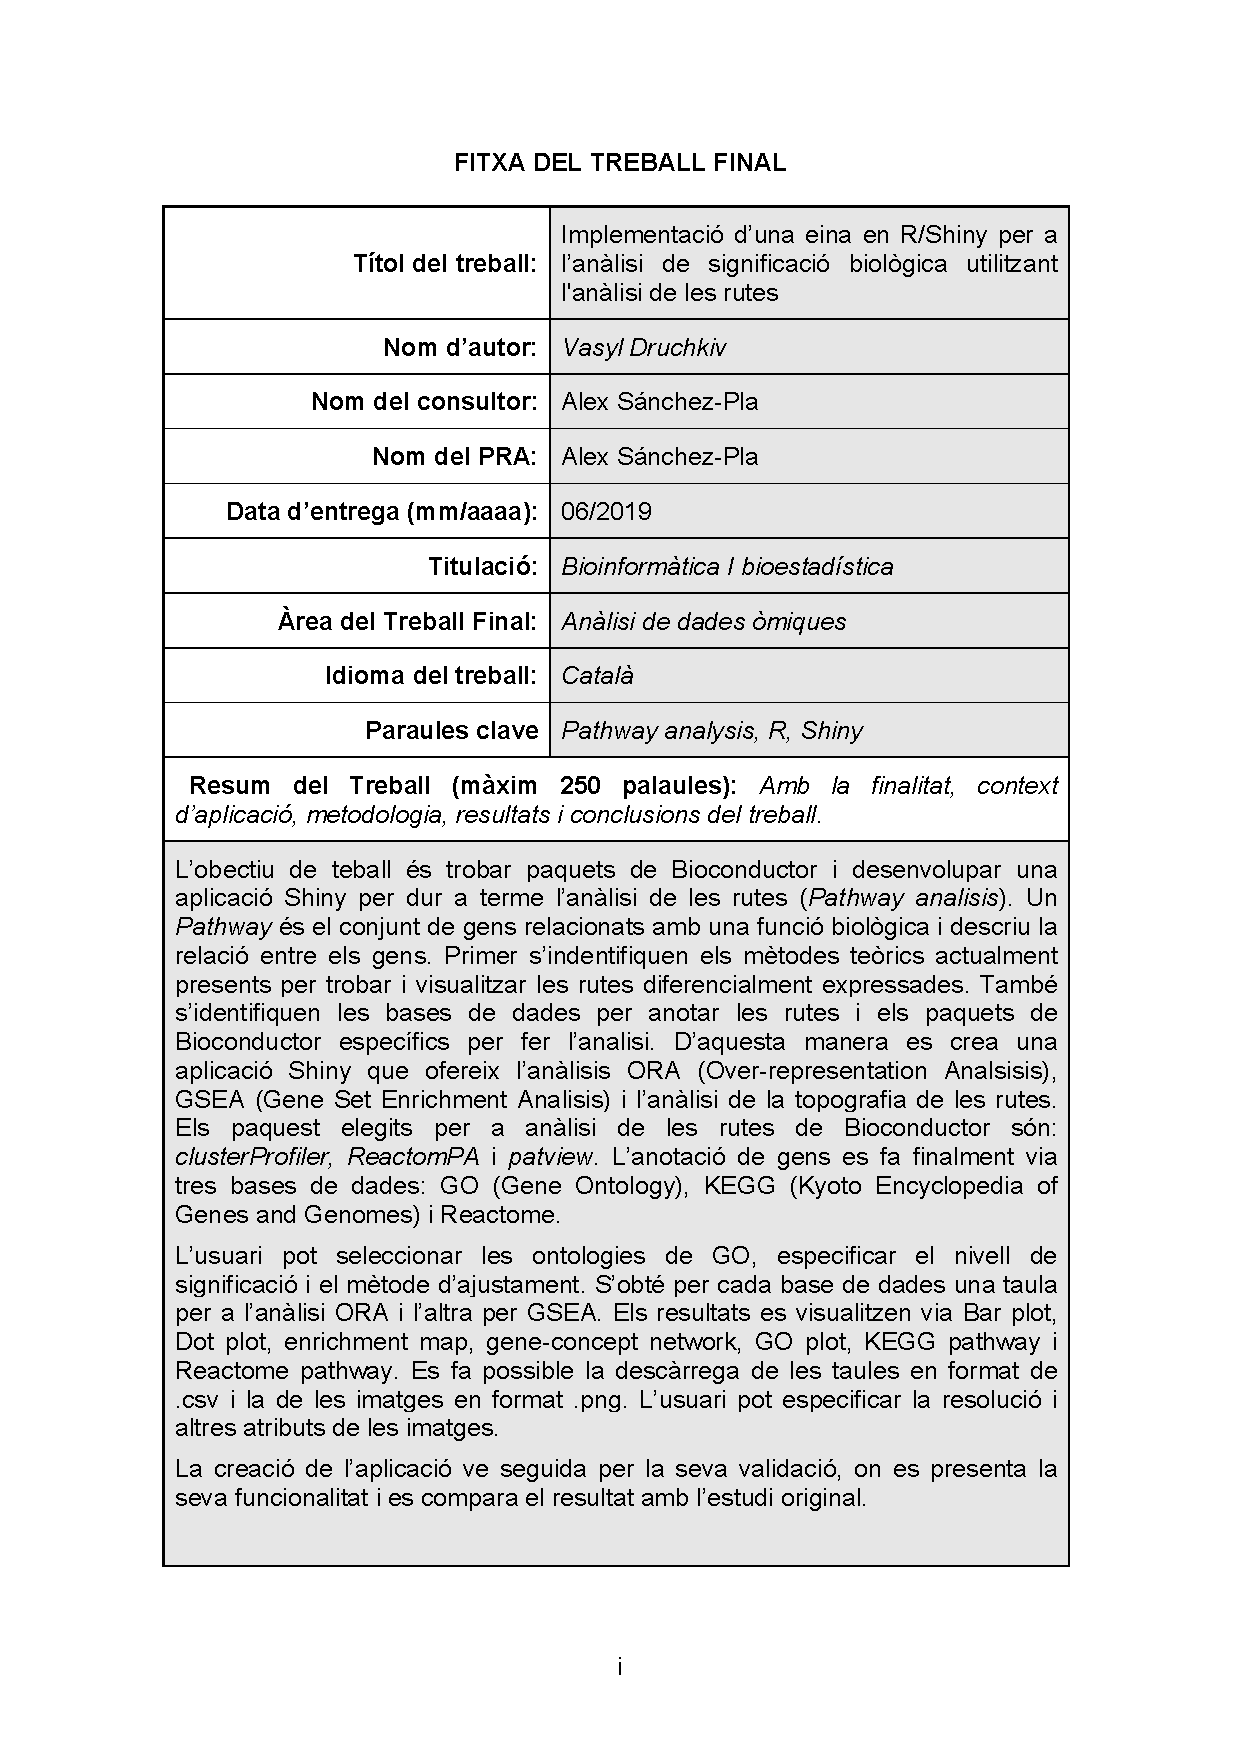
\includepdf[pages=-]{Abstract}


\tableofcontents                %% this produces the table of contents - you might have guessed :-)

\listoffigures

%% if myaddlistoftodos is set to "true", the current list of open todos is added:
\ifthenelse{\boolean{myaddlistoftodos}}{
  \newpage\listoftodos          %% handy if you are using todonotes with \todo{}
}{}                             %% with todonotes-package option "disable" you can get rid of any todo in the output

\mainmatter                     %% KOMA: marks main part using arabic page numbers and such; only available in scrbook


%----------------------------------------------------------------
%
%  File    :  thesis-style.tex
%
%  Author  :  Keith Andrews, IICM, TU Graz, Austria
% 
%  Created :  27 May 93
% 
%  Changed :  19 Feb 2004
% 
% styling and technical implementation adopted 2011 by Karl Voit
%----------------------------------------------------------------

%% defined an anvironment for the style Keith used to use:
\newenvironment{mykeithtabbing}[1]{%%
\begin{tabular}{lp{0.9\hsize}}
}{%%
\end{tabular}
}

\newcommand{\mybadgood}[2]{%%
\begin{mykeithtabbing}
{}\emph{Bad:}  & \sout{#1}  \\
\emph{Good:}   & #2  \\
\end{mykeithtabbing}
}



\chapter{Introducció}

El treball consistirà en el desenvolupament d'una aplicació per dur a terme l'anàlisi de les rutes (\textit{Pathway analysis}). Amb les rutes entenem un conjunt de gens que actuen junts per dur a terme un procès biològic. Així doncs aquest anàlisi permet donar més sentit a una expressió genètica diferencial entre les proves biològiques d'interès. Recordem que recents avenços tecnològics permeten mesurar els nivells d'expressió en una gran quantitat de gens, cosa que implica una gran quantitat de dades. Al nivell dels gens individuals es poden fer servir mètodes estadístics per comprovar si les diferències en les expressions entre els grups (proves biològiques) són estadísticament significatives. Per dotar encara de més sentit aquesta anàlisi és necessari agregar els resultats al nivell més raonable com ara al nivell de les rutes. Al final el que volem és comprovar si hi ha diferències estadísticament significatives entre les proves no al nivell dels gens perticulars sinó al nivell de les rutes. Tan com en el cas dels gens particulars també en el nivell de les rutes s'han desenvolupat mètodes estadístics específics \cite{khatri2012ten}. En aquest treball vull analitzar quins mètodes són i quins tenen més avantatges que d'altres. A part d'aquest component més biològic i teòric del treball he buscat la possibilitat d'implementar aquests mètodes d'anàlisi en una aplicació intuïtiva i d'un ús fàcil a la qual qualsevol científic que no disposi dels coneixements informàtics suficients per fer aquesta anàlisi podrà accedir gratuïtament. La plataforma que he utilitzat per crear l'aplicació és l'eina Shiny de Rstudio \cite{Shiny}.  La feina ha consistit en la cerca dels paquets de Bioconductor que inclouen els mètodes per l'anàlisi de les rutes, selecció dels paquets més apropiats i la seva integració en una aplicació Shiny amb una interfície atractiva. 

\section{Context i justificació del treball}
La justificació d'aquest tema ve de dues fonts diferents: d'una banda tinc un interès personal i d'altra banda entenc la importància de la meva aportació per a la comunitat científica. El meu interès personal és degut al fet que durant el màster he fet servir àmpliament el programa R però no he arribat a conèixer bé la creació d'una aplicació estadística amb Shiny. Per completar aquesta deficiència i entenent que aquesta eina és útil per al méu desenvolupament professional he buscat el tema que en requeria l'ús. Encara que hi ha algunes aplicacions de Shiny relacionats amb l'anàlisi de les rutes\footnote{Algunes splicacions existens de Shiny són: iDINGO \cite{class2017idingo}, ShinyGO \cite{ge2018shinygo}, PAEA \cite{clark2015principle}} i tanbé en altres plataformes \cite{reimand2019pathway}, elles no representen tota la diversitat dels paquest disponibles a Bioconductor. L'ús d'aquests paquets queda restringit per a experts en informàtica i estadística i per tant són difícilment accecibles per la gran part de la comunitat scientífica, de modo que seria convenient donar-hi més accessibilitat via una aplicació amb interfici visual. 


\section{Objectius}

Entre els objectius del treball podem distingir els general i els més especifics:
 
\subsection{Objectius generals}
\begin{enumerate}
\item Identificar els objectius i mètodes de l'anàlisi de les rutes (Bio/Stat)
\item Identificar els paquets de Bioconductor en R que s'aproximin als mètodes (Info)
\item Desenvolupar l'aplicació Shiny  amb els paquets escollits per aproximar el resultat als objectius de l'anàlisi de les rutes  (Info)
\end{enumerate}

\subsection{Objectius específics}
\begin{enumerate}
\item Biologia/Estadística
\begin{enumerate}
\item Buscar literatura sobre l'anàlisi de rutes
\begin{itemize}
\item Quins mètodes hi ha? Enumerar-los i explicar-los, especialment els tests estadístics.
\item Quines bases de dades es fan servir?
\item Determinar les opcions per visualitzar els resultats de l'anàlisi de les rutes.
\end{itemize}
\item Identificar les aplicacions existens i investigar què ofereixen
\item Analitzar els vignettes dels paquets de Bioconductor i provar-ne el seu ús localment amb R
\end{enumerate}
\item Informàtics
\begin{enumerate}
\item Crear i documentat un protocol (pipeline) de l'anàlisi utilitzant els paquets seleccionats. 
\item Identificar les dades experimentals per passar-les pel pipeline creat
\item Fer proves amb les dades seleccionades
\item Fer canvis en el protocol si és necessari
\item Integrar el pipeline a l'aplicació Shiny
\end{enumerate}
\end{enumerate}

\section{Enfocament i mètode de seguir}

Com es pot entendre dels objectius la feina ha consistit d'una banda en l'anàlisi teòrica dels mètodes disponibles actualment per a l'anàlisi de rutes, i d'altra banda en el desenvolupament d'una aplicació que incorporarà aquests mètodes. El mètode triat per per aconseguir aqusts objectius era el mètode simultani on la programació es desenvolupava alhora de l'anàlisi dels conceptes teòrics. D'aquesta manera he seguit auqests pasos:

\begin{enumerate}
\item Trobar un mètode teòric que proporcioni un resultat interessant;
\item Buscar en Bioconductor aquest mètode;
\item Repetir 1 i 2 fins que el conjunt dels mètodes facin l'anàlisi de les rutes complet. 
\item Quan tots els mètodes son triats dissenyar un protocol;
\item Aplicar el protocol a les dades independents;
\item Comparar els resultats amb els estudis d'on provenen les dades;
\item Ajustat últimament el protocol;
\item Desenvolupar l'aplicació
\end{enumerate}
 
S'ha d'emfatitzar el punt 5 i 6. Era essencial trobar les dades que s'utilitzin per fer les probes durant la fase de desenvolupament de \textit{pipeline}. Les dades havien de provenir d'uns resultats ja publicats per poder comparar-los amb els resultats obtinguts amb el programari elaborat. 

\section{Planificació del treball}

Es van definir les tasques següents per aconseguir els objectius:

\begin{enumerate}
\item Cerca de la literatura sobre els mètodes de l'anàlisi de les rutes;
\item Relacionar els mètodes trobats en 1 amb els paquets actuals de Bioconductor;
\item Decidir sobre quals resultats son més interesants per a una aplicació Shiny i desenvolupar un protocol de l'anàlis (\textit{pipeline}) que formarà la base de l'aplicació. Documentar el protocol;
\item Buscar 3-5 exemples de dades i fer proves aplicant el protocol i comparant els resultats amb els resultats publicats sobre aquestes dades (si n'hi ha);
\item Fer últims canvis en el protocol;
\item Dissenyar i programar l'aplicació de Shiny;
\item Pupblicar l'aplicació en web;
\item Tancar la memòria i fer la presentació per la defensa.
\end{enumerate}

Aquestes tasques he distribuït de modo següent: 

\begin{figure}[H]
\caption{Gantt Plot}
\centering
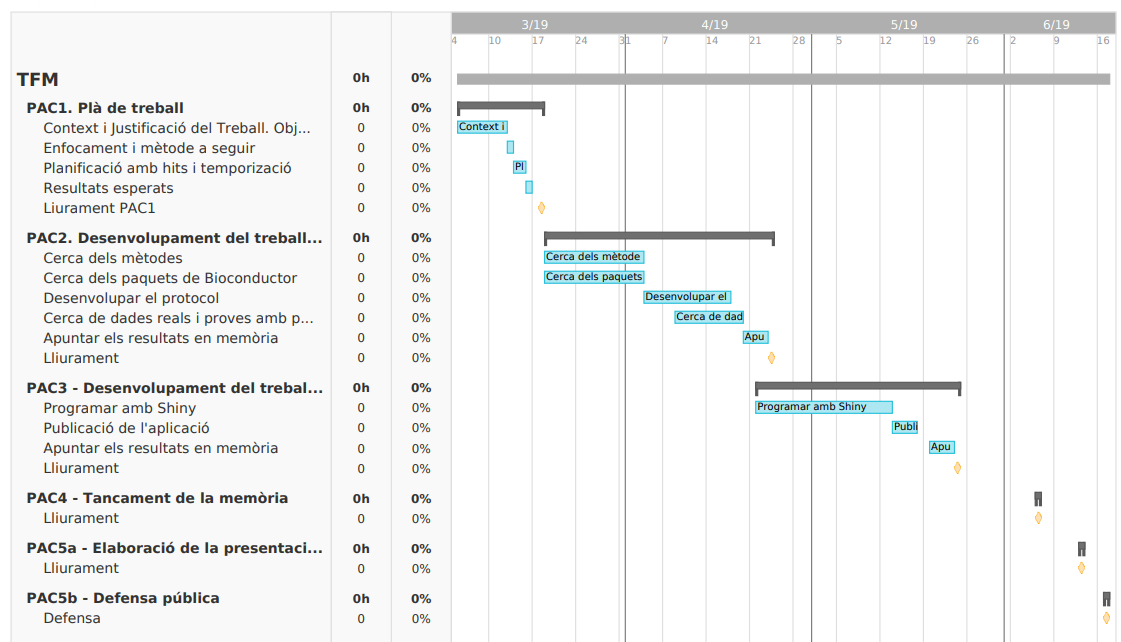
\includegraphics[width=0.9\textwidth]{figures/GanttPlot}
\end{figure}

Els treballs previstos per plà docent i realizades i entregades a temps eren esl següents: 

\begin{center}
 \begin{tabular}{||c | l | c | c||} 
 \hline
 Activitat & Nom d'activitat & Data d'inici & Data d'entrega  \\ [0.5ex] 
 \hline\hline
 PAC0 & Definició dels continguts del treball & 20/02/19 & 04/03/2019 \\ 
 \hline
 PAC1 & Pla de treball & 05/03/19 & 18/03/19 \\
 \hline
 PAC2 & Desenvolupament del treball - Fase 1 & 19/03/19 & 4/04/19 \\
 \hline
 PAC3 & Desenvolupament del treball - Fase 2 &  25/04/19 & 20/05/19 \\
 \hline
 PAC4 & PAC4 - Tancament de la memòria & 21/05/19 & 05/06/19 \\
 \hline
\end{tabular}
\end{center}

\section{Breu sumari dels productes obtinguts}

El producte central obtingut és l'aplicació Shiny que actualment es pot descargar del meu repositori a Github (veure l'apartat instal·lació de l'aplicació).  Al mateix repositori es pot trobar tot el material relacionat amb la creació de l'aplicació: els arxius de latex per a les proves d'avaluació continuada, les captures de pantalla utilitzades en aquestes PACs, també el paquet modificat \helvetica(pathview) que es diu \helvetica{pathviewPatched} i que permet guardar les imatges de les rutes al directori especificat.

\section{Breva descripció dels capítols del treball}

Al primer capítol més teòric presentaré els mètodes més relevant per a anàlisi de les rutes. Començaré però amb el context d'investigació de l'expressió genètica i més específicament amb l'anàlisi de microarrays per poder situar millor l'anàlisi biològic de les rutes. Donat les dades d'experiment explicaré brevament quins resultats habitualment s'en deriven. Veurem que aquests resultats són la llista de gens diferencialment expressats i el magnitud d'expressio diferencial mesurada via \textit{logRatio} per tots als gens. 

Seguidament investigaré quines estratègies existen per dur a terme l'anàlisi de les rutes. Aquí identificaré tres estratègies generals: l'anàlisi \Gls{ORA} (Over-Representation Analisis), FCS (Functional Class Scoring) i l'anàlisi topològic de les rutes. Veurem que aquests anàlisis accepten com les dades d'entrada els resultats obtinguts via \textit{microarrays} descrits anteriorment. Per poder fer us d'aquestes dades però és necessari anotar els gens d'experiment. Per aquest motiu presentaré els tres bases de dades més relevant per anotar els gens amb objectiu de fer anàlisi de les rutes: GO, KEGG i Reactome.

Finalment parlaré sobre els mètoded \gls{ORA} i GSEA més detalladament enfocant especialment als resultat que preporcionen. També descriure brevament la visualitzacions possible de les rutes. Per acabar presentaré el protocol que utilitzaré per crear l'aplicació.

Al capítol següent explicaré els paquets de Bioconductor per dur a terme l'anàlisi descrit al capítol anterior i el modo amb el qual he fet l'aplicació accessible. Veurem que al moment de redacció d'aquesta memòria l'aplicació es pot ser descargada de GitHub utilitzant el paquet \helvetica{devtools} de R. S'intentarà però habilitat l'aplicació  per a internet utilitzant el servidor de l'area d'estadística i bioinformàtica. 

Al capítol següent presentaré l'aplicació. Aquí utilitzaré les dades del paquet clusterProfiler per mostrar el funcionament d'aplicació: des de pujament de les dades fins obtenció de les representacions gràfiques.

Al capítol següent intentaré validar l'aplicació. Parlaré dels problemes a l'hora de trobar les dades preprocessades i presentaré les dades amb les quals en faig intent i em concentraré més en l'estudi de l'expressió gènica dels ratolins midificats genèticament de tal manera, que el seu gen  Zbtb7b està silenciat. Veurem que els resultats obtinguts amb l'aplicació s'assemblen als resultats descrits al \textit{paper} original. 

Per acabar faré conlusions del meu treball.
 
\chapter{El marc teòric}

\section{Les dades d'expressió genètica}
Les dades d'entrada per a l'anàlisi de les rutes provenen típicament de l'anàlisi de \textit{microarrays} d'ADN, que produex dades d'expressió de $m$ gens (variables) per a $n$ mARN mostres (observacions). Les dades com aquestes poden resultar d'un estudi d'investigació sobre efectes d'una proteïna com per exemple a l'estudi de \cite{li2017zbtb7b} on s'investiga la correlació entre la proteïna Zbtb7b (Zinc finger and BTB domain-containing protein 7B) i la formació de teixit adipós marró i beix i d'aquesta manera influex sobre fisiologia metabòlica. En aquest cas l'objectiu és comparar teixits de dos ratolins un de tipo salvatge i l'altre amb el gen ZBTB7B silenciat i investigar quins gens són diferencialment expressats entre aquestes mostres biològiques. 

Al gràfic següent veiem l'estructura habitual d'un experiment de \textit{Microarray}.

\begin{figure}[H]
\centering
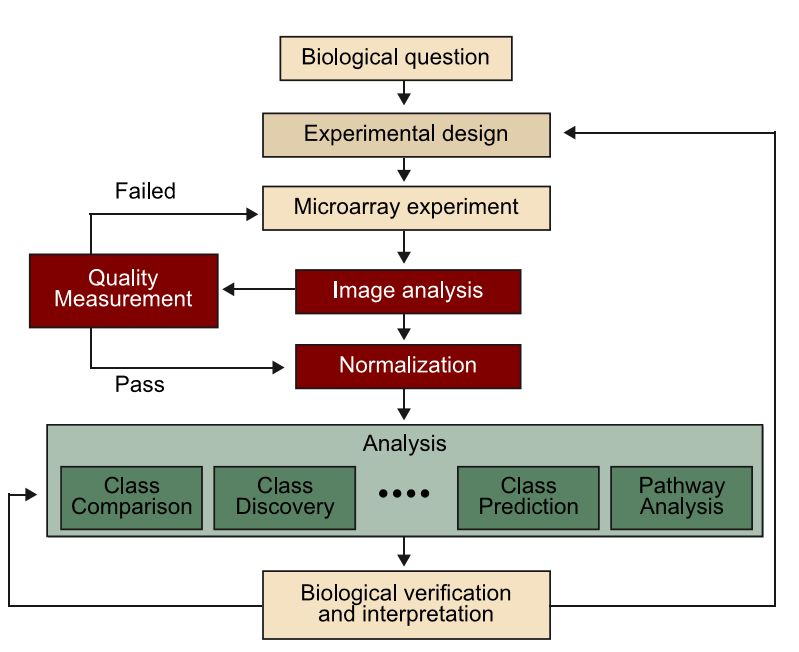
\includegraphics[width=0.9\textwidth]{figures/Pipeline_Microarray.jpg} 
\caption{El procès d'anàlisi de microarrays}
\end{figure}

El \textit{pipeline} de l'anàlisi consisteix doncs en plantejament d'una pregunta i un disseny experimental a partir del qual és fa l'experiment de \textit{microarrays}. El producte d'experiment són bàsicament les images d'intensitats que es tradueixen als valors numèrics. Habitualment aquests valors són encara \textit{raw values} i han de ser processats adequadament. Aquest processament inclou el control de qualitat d'imatges i la normalització dels valors d'intensitat per reduir la variabilitat tècnica. Finalment les dades normalitzades s'utilitzen per a l'anàlisi estadístic. Habitualment la mesura natural per comparar les mostres és el \textit{log ratio} el qual podem denomiar alternativament \textit{logFC} on \textit{FC} es refereix a \textit{fold change}. Hi ha diversos tests estadístics per comprobal les difrències entre les mostres. En el cas de l'array d'un color podem fer servir tan els metodes paramètrics com ara el test T o mètodes del modelatge lineal o bé mètodes nonparamètrics com ara la proba de Mann-Whitney. El test adequat dependrà bàsicament de la distribució de les dades. El resultat d'aquest anàlisi serveix com a base per a interpretació biològica dels resultats d'experiment. Per poder fer sentit de les dades d'expressió i de l'anàlisi estadístic al nivell de gens és imprescindible fer un anàlisi a nivell de les categories de gens o les rutes. Per aquest anàlisi es necessita, com ho veurem a l'apartat següent, una llista ordenada de les expressions relatives (\textit{logFC}) i una subllista de gens que hem identificat mitjançant els tests estadístics com a diferencialment expressats.

En aquest treball m'ocupo de l'últim pas d'experiment d'escrit, més especificament amb l'anàlisi de rutes (\textit{Pathway analysis}).

La vista general de l'anàlisi de les rutes ofereix el gràfic següent:

\begin{figure}[H]
\centering
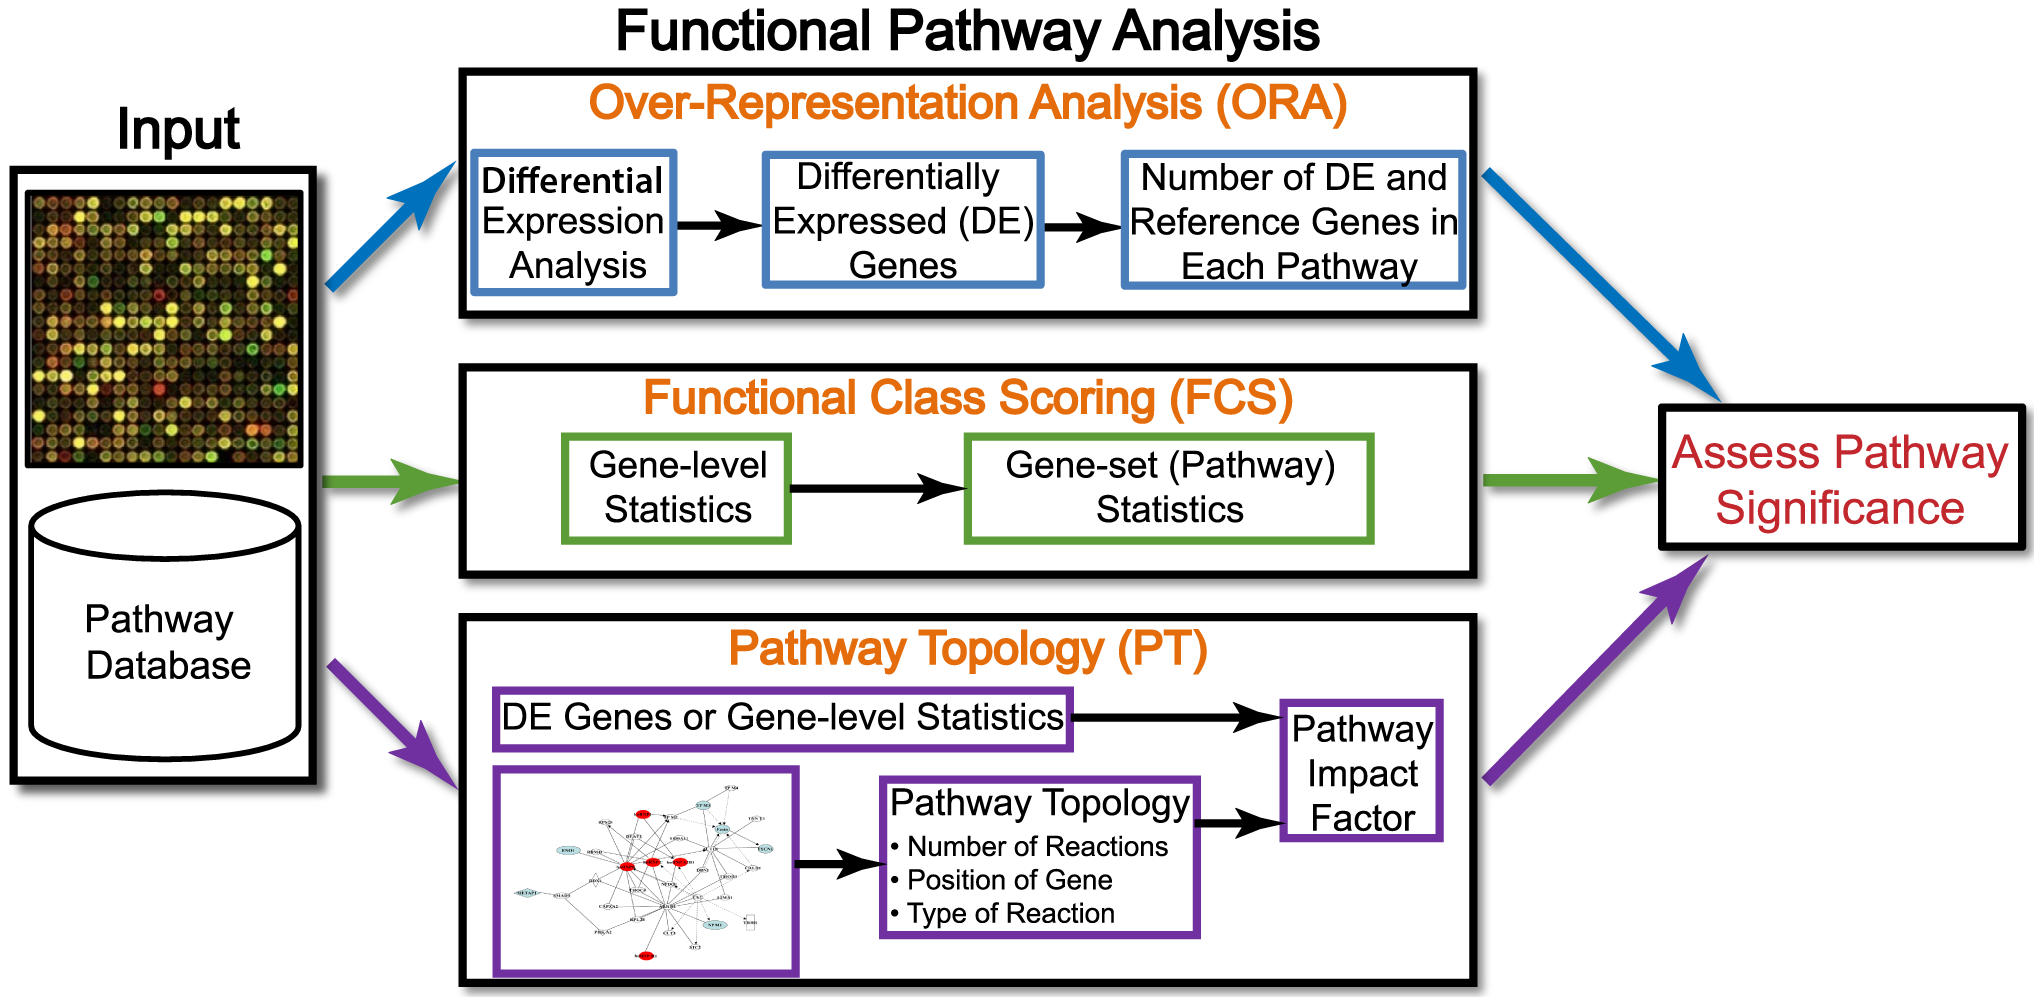
\includegraphics[width=0.9\textwidth]{figures/Pipeline_Pathway.png} 
\caption{El procès d'anàlisi de les rutes}
\end{figure}

A part de les dades d'expressió, de les quals he parlat anteriorment, l'analisi requereix com a \textit{input} també la base de dades de les rutes. De les dades que utilitzaré a la meva aplicació en parlaré a la secció següent. Per ara hes important entendre que els resultats d'expressió s'anoten a les bases de dades existents per comprobar si els gens sobre o sotaexpressats pertanyen a unes rutes específica. Per comprobar aquesta, o millor dit, aquestes hipòtesis (per que hi hauran hipòtesis múltiples) s'han establert tres grups dels mètodes:

\begin{itemize}
\item \textbf{Over-Representation Anaysis (ORA)}.
Aquest anàlisi necessita la preselcció dels gens diferencialment expressats (DE) i compara la freqüència dels gens de la ruta d'interès en la mostra dels gens diferencialment expessats i la freqüencia dels gens de la ruta a la distrinució de fons (\cite{boyle2004go}. 
\item \textbf{Functional Class Scoring (FCS)}
Per a aquesta anàlisi no necessitem cap preselecció dels gens diferencialment expressats (DE) sinó ja basta amb tenir les estadístiques a nivell de gens, que al cas de l'aplicació és el \textit{logFC}. Hi ha diversos mètodes que generen una estadística per a tot conjunt de gens d'una ruta i la comparen amb una distribució teòrica per a constrastat la hipòtesi nulla. Els métodes es diferencien bàsicament en calculació de la puntuació d'enriquement que poden incluir l'estadística de Kolmogorov-Smornov, la suma, media o mediana d'estadistiques al nivell de gens etc. \cite{khatri2012ten}. O bé es poden diferencia en calculació de la distribució teòrica: aquí alguns mètodes utilitzen la permutació de les mostres  o de gens, cosa que implica dos hipòtesis diferents.  
\item \textbf{Pathway Topology (PT)}.
Aquest mètode enfoca la posició de gens diferèncialment expressats en la ruta i d'aquesta manera utilitza el coneixement de les bases de dades més àmplicament. Per exemple, si una ruta està activada per un sol producte genètic o mitjançant un reseptor i si aquesta proteïna particular no està produïda, la ruta estarà molt afectada, o fins i tot apagada. Més especifivacment, si el receptor d'insulina no és en la ruta d'insulina (\url{https://www.genome.jp/dbget-bin/www_bget?hsa04910}) tota la ruta serà desactivada (\cite{tarca2008novel}). D'altra banda si un nombre de gens està involucrar en la ruta però apareixen riu abaux el seu efecte podria ser menys important. A més a més també el nombre de coneccions amb altres gens a la ruta podria ser important \cite{rahnenfuhrer2004calculating}. O fins i tot leas estadístiques que incorporen factors diferents com ara la posició, el tipo d'interacció etc. \cite{draghici2007systems}. Aquesta idea l'he implementat en l'aplicació afegint les rutes dibuixades de KEGG i Reactome, on els gens estan emfatitzats d'acord amb els \textit{logFCs} obtinguts mitjançant l'experiment.

En els capítols següents presisaré més formal els métodes d'ORA i GSEA i també descriuré algunes possibilitats per visualitzar les dependències de gens dins de les rutes específiques i també les relacions entre les rutes diferencialment expressades.

\end{itemize}


\section{Annotació dels gens}

Com veurem més endavant per a anàlisi de les rutes és imprescindible tenir com a referència anotacions dels gens. Per a aplicació he utilitzat tres bases de dades: Gene Onthology (GO), Kyoto Encyclopedia of Genes and Genomes (KEGG) i Reactome. clusterProfiler també inclou WikiPathways però per raons de temps he decidit focusar-me només a les tres mencionts anteriorment. Aquestes bases de dades no són però úniques. N'hi ha també altres com per exemple \textit{Pathway Studio pathways} o \textit{IPA} amb inconvenient que són comercials i no gratuites. 

\subsection{Gene ontology}
Gene Ontology \cite{gene2004gene} dona tan un vocabulari estructurat i controlat (ontologies) com la classificació que cobreix alguns dominis de la biologia molecular i cel·lular. És una base de dades gratuïta per a anotació de gens, el seu producte i les seqüències. El projecte GO proporciona ontologies per a descriure els atributs dels productes de gens als tres dominis separats de la biologia molecular:
\begin{enumerate}
\item \textbf{Molecular Function (MF)}. Aquest domini descriu activitats al nivel·l molecular. És important entendré que el terme ``molecular function'' representa més les activitats i no pas les entitats (com per exemple molecules o complexos) que fan aquestes accions i a més a més no espeifíquen quan o a quin context l'acció té lloc. Un exemple podria ser \textit{catalytic activity} o un terme més específic \textit{adenylate cyclase activity}.
\item \textbf{Biological Process (BP)}. Aquest domini descriu els objectius biològics aconseguits per una o conjunt de les funcions moleculars. Un exemple d'un procès biològic ampli podria se \textit{DNA repair}. Un exemple més específic podria se \textit{pyrimidine nucleobase biosynthetic process}. 
\item \textbf{Cellular Component (CC)}. EL CC descriu l'emplaçaments al nivell d'estructures subcel·lulars (com \textit{mitocondri}) i els complexos macromoleculars (com \textit{ribisomes}) on el producte de gen fa la seva funció.
\end{enumerate}

Dins de cada ontologia, els termens tenen tan una definició de text com un identificador únic. El vocabulari està estructurat en una classificació que manté les relacions ``is-a'' i ``part-of'' i ``regulates''. Aquestes relacions les descriu amb més detall més endavant en la secció dedicada al gràfic acíclic de GO termes.

\subsection{KEGG}
La base de dades KEGG és la col·lecció del mapes dibuixades manualment que representen el coneixemnet sobre interacció molecular dividit eb set dominis principals:
\begin{enumerate}
\item Metabolism
\item Genetic Information Processing
\item Environmental Information Processing
\item Cellular Processes
\item Organismal Systems
\item Human Deseases
\item Drug Development
\end{enumerate}

Els mapes són dibuixades amb un software específi (KegSketch) que genera un arciu KGML+. Aquest arxiu és un arxiu SVG que conté els objectes gràfics que són associats amb els objectes KEGG. Els objectes gràfics bàsics de les rutes KEGG són:
\begin{itemize}
\item caixes: gens o el seu producte
\item cercles: altres molècules
\item línies: reaccions
\end{itemize}
 
El significat més detallat d'aquests elements el presentaré a la secció dedicada a les rutes KEGG.

\subsection{Reactome}

Reactome és una base de dades gratuitament accecible i manualment curada per a reaccions i rutes biològiques. Al centre de Reactome són reaccions que es definexen com qualsevol esdeveniment molecular com ara unió, fosforilització, catàlisi bioquèmic, transport molecular o esdeveniments moleculars espontani. Aquestes reaccions involucren qualsevol molècula, però més típicament passen entre proteïnes i les molècules petites. Encara que els mapes de Reactome disponibles online contenen una relació entre les molecules més detallada el paquete de Bioconductor que utilitzaré per generar els mapes visualitza només la conecció bàsica entre els gens. 

\section{ORA}

L'anàlisi de sobreexpressió és una tècnica d'identificació de les rutes significativament enriquides en la mostra d'interès. 

El paper original que se cita habitualment quan es parla d'anàlisi d'expressió genètica és de \cite{boyle2004go}. El mètode estadístic descrit consisteix bàsicament en els passos següents:

\begin{enumerate}
\item \textbf{De tots els gens de la mostra seleccionar un grup de gens que es considera que són significativament expressats.}

Els criteris de selecció poden basar-se en \textit{log ratios} i/o en el valor de p provinent d'un test estadístic. \textit{Log ratios} donen la magnitud amb la qual un gen és sobre o sotaexpressat. Les diferències entre els grups però són el resultat d'un procès estochàstic i per tant hem d'intentar de minimitzar el risc de prendre decisions falses. El valor de p representa la probabilitat d'aquest risc i per tant dona certa confiança sobre la significació de les diferències observades.

\item \textbf{Determinar si algunes rutes anoten la llista especificada de gens amb la freqüència més alta que la que s’esperaria per casualitat.} 

El test estadístic es basa en la distribució hipergeomètrica: 

$$p = 1 - \displaystyle\sum_{i = 0}^{k-1}\frac{{M \choose i}{{N-M} \choose {n-i}}} {{N \choose n}}$$

En aquesta equació $N$ és el nombre total de gens en la distribució de fons, $M$ és el nombre de gens dins d'aquesta distribució que són anotats a la ruta d'interès, $n$ és el nombre total en la llista especificada de gens i $k$ és el nombre de gens dins d'aquesta llista que són anotats a la ruta. La distribució de fons pot ser o bé tots els gens en la base de dades d'anotació o bé tots els gens de l'experiment.

El valor de P obtingut amb aquesta fòrmula dona la probabilitat de veure el nombre $x$ de gens de la llista relacionats amb la ruta específica en la llista del nombre total de gens $n$ donat la proporció de gens relacionats amb aquesta ruta en la distibucó de fons.
\end{enumerate}

L'aplicació utilitza aquesta idea i calcula una taula amb els camps següents:


\begin{itemize}
\item \underline{Description}. El nom del terme GO;
\item \underline{GeneRatio}. El quocient $\frac{M}{N}$ on $M$ és el nombre dels gens diferencialment expressats que pertanyen al conjunt de gens i $N$ és el nombre total dels gens diferencialment expressats 
\item \underline{BgRatio}. El quocient: $\frac{k}{n}$ on $k$ és el nombre dels gens del conjunt d'interès en la distribució de fon i n és el nombre total dels gens en la distribució de fons;
\item \underline{pvalue}. Valor de p basat en la distribució hipergeomètrica descrita anteriorment.
\item \underline{p.adjust}. El valor de P ajustat. L'usuari pot seleccionar el mètode d'ajustmanent.
\end{itemize}


\section{GSEA}

Amb l'anàlisi GSEA podem analitzar els resultats d'un experiment d'expressió per a dos grups. Aquí els gens són ordenats basant-se en la correlació entre la seva expressió i la separació entre les classes. Aquest llistat ordenat $L$ el podem crear utilitzant els \textit{logRatios}.

Donat el conjunt definit dels gens $S$, que pertanyen per exemple al mateix terme de Gene Ontology, l'objectiu de GSEA és determinar si els membres de $S$ són distribuïts aleatòriament en el $L$ o es troben més al cap o a la cua. S'esperaria que els gens relacionats amb la separació fenotípica mostraran aquesta última distribució. 

L'anàlisi GSEA consisteix en tres passos subramanian2005gene:

\begin{enumerate}
\item Càlcul de la puntuació d'enriquement (\textit{ES: Enrichment Score}). La puntuació està calculada anant per la llista i augmentant la suma corrent sempre quan es troba un gen que pertany a $S$ o, al contrari, restant-la quan el gen no forma part del conjunt $S$. La puntuació és la desviació màxima del zero observada en aquet camí. L'estadística obtinguda és l’estadística de Kolmogorov-Smirnov amb pesos.

\item Estimació del nivell de significació per a la puntuació \textit{ES}. El valor de P nominal es pot obtenir mitjançant o bé la permutació de les classes o bé la permutació de gens, on l'estadística \textit{ES} observada es compara amb la distribució obtinguda amb permutació. Els dos modos de permutació comproven les hipòtesis diferents. Mentre la permutació de gens comprova la hipòtesi que \textit{els gens en la ruta com a màxim són diferencialment expressats com els gens fora de la ruta},
la permutació de les mostres implica la hipòtesi que cap de gens en la ruta són diferencialment expressats. Es diferencies doncs en tractament de gens fora de la ruta. A l'aplicació es fa ús de la permutació de gens degut bàsicament a la selecció dels paquets de Bioconductor per a aplicació.


\item Càlcul del valor de P ajustat. El valor de P nominal s'ajusta per controlar l'error global que es produeix com a resultat de les comparacions múltiples.
\end{enumerate}

\begin{figure}[H]
\centering
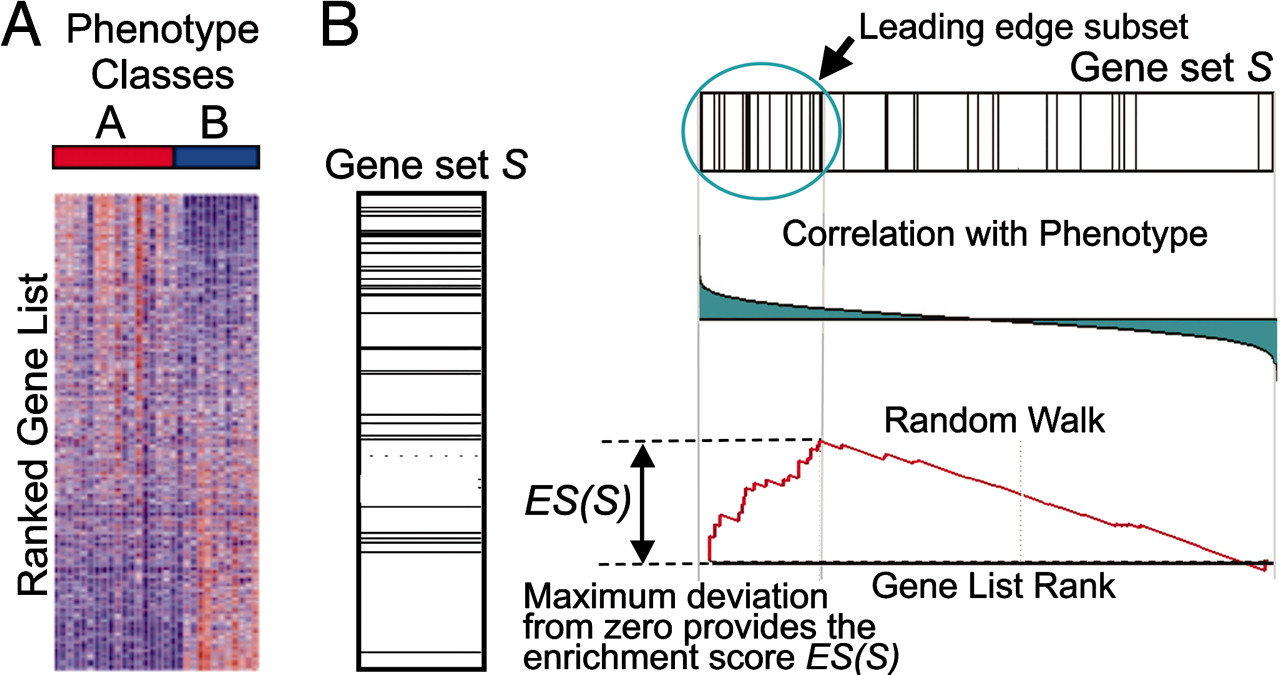
\includegraphics[width=0.9\textwidth]{figures/GSEA_Method.jpg} 
\caption{El mètode GSEA}
\end{figure}

L'aplicació que he desenvolupat agafa aquesta idea i calcula la taula que inclou les estadístiques següents:

\begin{itemize}
\item \underline{enrichmentScore}. Enrichment score per al conjunt dels gens. Amb altres paraules: el grau amb el qual el conjunt dels gens està sobreexpressat a dalt o a baix del llistat ordenat dels gens en les dades d'expressió.
\item \underline{NES}. Normalized enrichment score. La puntuació per al conjunt de gens després de ser normalitzat tenint en compte tots els conjunts de gens analitzats (la seva mida i la seva correlació amb les dades d'expressió). Aquesta puntuació ajuda a comparar els resultats entre els conjunts de gens.
\item \underline{pvalue}.El valor de p nominal.
\item \underline{p.adjust}. El valor de p ajustat.
\item \underline{leading\_edge}
\begin{itemize}
\item \underline{Tags}. El percentatge de les ocurrències de gens del conjunt específic abans (per als ES positius) o després (per als ES negatius) del cim en la puntuació corrent d'enriquiment. Aquest valor indica el percentatge dels gens que contribueixen a la puntuació d'enriquement. 
\item \underline{List}. El percentatge dels gens en el llistat ordenat de tots els gens abans o després del pic en la puntuació corrent d'enriquiment. Aquest valor ens indica on exactament el pic es produeix. 
\item \underline{Signal}. La fortalesa del senyal d'enriquiment que combina els dos valors anteriors.
\end{itemize}
\item \underline{rank}. La posició del pic en la llista ordenada dels gens. Els conjunts dels gens més interessants assoleixen el seu màxim o bé al principi o al final de la llista ordenada. Vol dir que tenen aquest valor o bé molt baix o bé molt alt.
\end{itemize}

\section{L'anàlisi topològic de les rutes}
Tan \gls{ORA} com GSEA no visualitzen les relacions entre les rutes i entre els gens dins de les rutes. Els avenços en anotació manual de les bases de dades disponibles (GO, KEGG i Reactome) contenen però aquesta informació i l'aplicació, gràcies al paquet \helvetica{clusterProfiler}, hi treu l'avantatge i visualitza aquestes relacions més detalladament. 

\subsection{El mapa d'enriquement}

Navegant a la categoria \textbf{Enrichment plot} l'usuari obté el mapa d'enriqument. El mapa organitza les rutes en una xarxa amb les línies que connecten les rutes amb els gens solpats. D'aquesta manera les rutes amb gens en comú s'agrupen més a prop l'una de l'altra.

\subsection{Gene-Concept-Network}

L'anàlisi \gls{ORA} no visualitza per si sola els gens que contribueixen al fet que la ruta sigui diferencialment expressada. Amb la xarxa de gens-concepte es pretén visualitzar els gens al voltant dels conceptes on els gens poden ser connectats amb les rutes (conceptes) diferents. D'aquesta manera es fa possible identificar les associasions biològiques més complexes entre les rutes mitjançant els gens. 

\subsection{GOplot}
%Per a mès informació http://geneontology.org/docs/ontology-relations/

El gràfic de GO està organitzat com direccional acíclic gràfic (Directed Acyclic Graph). Una manera útil de veure els resultats és mirar com els termes GO estan distribuïts per aquest gràfic. L'aplicació ensenya el gràfic GO induït pels els gens més significatius. El gràfic mostra tres relacions possibles entre les rutes: 
\begin{enumerate}
\item \textit{is a}: Si dèiem que A \textit{is a} B, volem dir que A és un subtip de B. Per exemple el cicle mitòtic de la cèl·lula \textit{is a} cicle de la cèl·lula. 
\item \textit{part of}: Aquesta relació s'utilitza per representar la relació entre una part i el tot. Aquesta relació entre A i B existeix nomès si B és necessàriament una part d'A: quan B existeix, ho fa només com una part de B i la presència de B implica la presència d’A.
\item \textit{regulates}: La relació descriu el cas on un procès afecta directament la manifestació de l'altre procès.
\end{enumerate}

Els conceptes al llarg del gràfic són marcats amb color depenent si són estadísticament significatius o no.

\subsection{KEGG Pathway}
%Per a més informació sobre l'anotació https://www.genome.jp/kegg/document/help_pathway.html
Aquest gràfic mostra les relacións entre els gens dins de la ruta específica. Els gens són remarcats amb el color depenent de l'expressió diferencial mesurada amb LogRatios. Per poder interpretar el gràfic és útil tenir present l'anotació següent:

\begin{figure}[H]
\centering
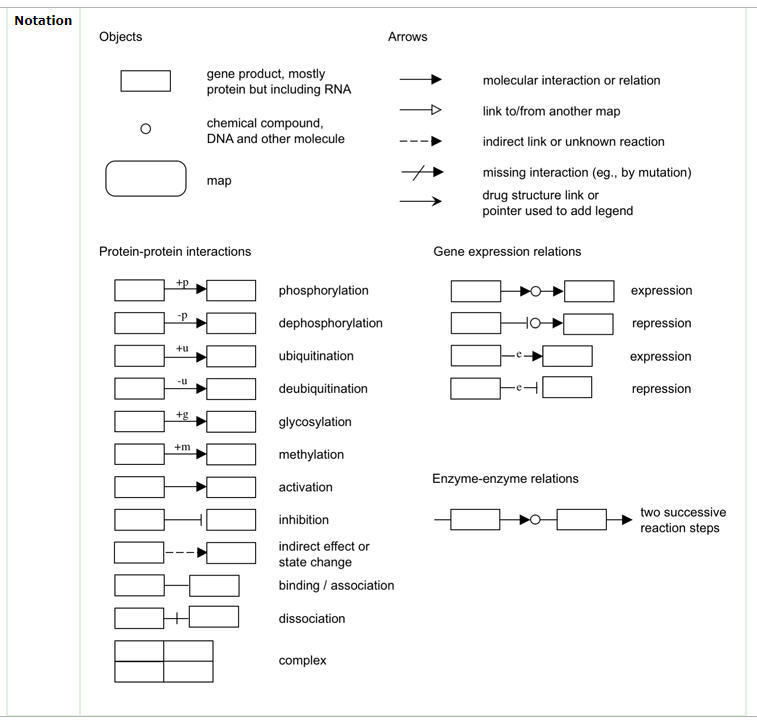
\includegraphics[width=0.9\textwidth]{figures/Annotation_KEGG.jpg} 
\caption{L'anotació de les relacions dins de les rutes KEGG}
\end{figure}

\subsection{Reactome Pathway}

Les rutes de Rectome són similares a les rutes de KEGG. La seva implementació amb Bioconductor, com ho veruem properament, no visualitza les rutes originales mostrades per \href{https://reactome.org/PathwayBrowser/}{Pathway Browser} de Reactome. La visualització amb al paquet \helvetica{ReactomePA} és més modesta i ofereix només les relacions nominals sense mostrar direcionalitat, com ho fa el gràfic de la ruta original de Reactome. Tot i així podem identificar quantes coneccions amb altres gens de la ruta tenen els gens diferencialment expressats i d'aquesta maner intuir la seva importancia relativa.  

En canvi a Goplot i les rutes KEGG les relacions entre els gens dins les rutes Reactome són més senzilles. Aquí les relacions són mostrades només amb les línies, on es pot interpretar només la distància entre els gens. 
%https://reactome.org/userguide/pathway-browser

\section{Desenvolupament del protocol}

Tenint en compte el marc teòric he intentat dessenyar l'aplicació que ofereixi els mètodes com ara ORA, GSEA i algunes visualitzacions de la topografia de les rutes. Igual amb quina base de dades l'usuari vol anotar les dades d'expressió l'usuari podrà decidir quin métode voll aplicar. En el millor dels casos l'usuari faria els dos mètodes \gls{ORA} i GSEA. Això implicaria la disponibilitat de dos arxius: l'arxiu amb tots els gens (Universe) i l'arxiu amb el grup de gens diferencialment expressats (Gene set). Si l'usuari vol fer només l'anpalisi GSEA haurá de pujar només l'arxiu amb tots els gens. Una vegada seleccionada l'estratègia l'usuari puja els arxius necessaris i gener el resultat de \gls{ORA} i/o GSEA aplicant uns critèris com ara selecció d'ontologia en ORA, valor de P com al filtre de visualització de les rutes més significatives, i el mètode d'ajustament.

\begin{figure}[H]
\centering
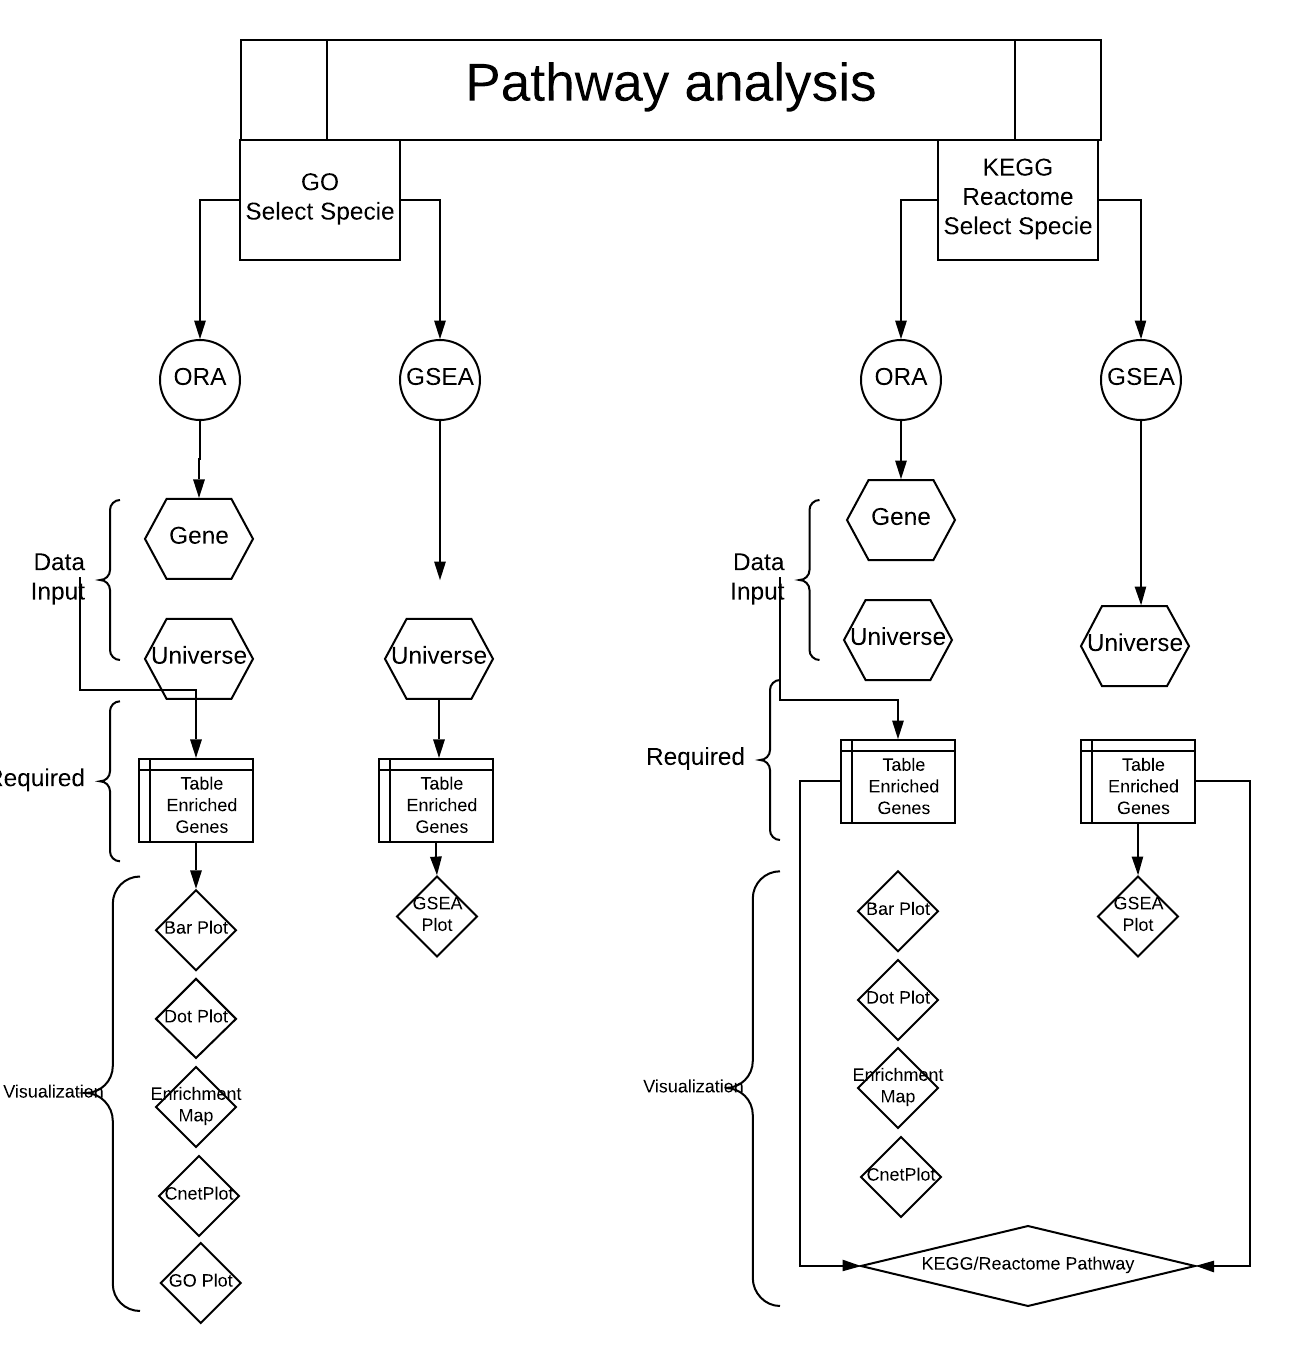
\includegraphics[width=.9\textwidth]{figures/LucidChart} 
\caption{Lucidchart per a l'aplicació}
\end{figure}

D'aquí podem definir per exemple el protocol:
\begin{enumerate}
\item Decidir quin anàlisi vol fer: GO, KEGG o Reactome
\item Seleccionar l'espècie de referència
\item Decidir quin mètode vol implementar: \gls{ORA} o GSEA i respectivament pujar les dades necessàries.

$\rightarrow$ Per a anàlisi GO tots dos arxius són necessaris: Gens Seleccionats (Gene) i Tots els gens (Universe). 

$\rightarrow$ Per a l'anàlisi KEGG o Reactome les dades necessàries varien: Pel mètode \gls{ORA} l'arxiu amb els gens seleccionats és suficient. Dos arxius són necessaris pel mètode GSEA.
\item En el cas que volguem fer l'anàlisis \gls{ORA} seleccionar a l'apartat corresponent (GO, KEGG o Reactome) la pestanya \gls{ORA} i definir els criteris.

$\rightarrow$ Els gràfics: Bar Plot, Dot Plot Enrichment Map, Cnet Plot, GO Plot (en cas d'anàlisi GO) i els gràfics de les rutes (KEGG/Reactome) es calculen automàticament

\item En el cas que volguem fer l'anàlisi GSEA seleccionar a l'apartat corresponent (GO, KEGG o Reactome) la pestanya GSEA i definir els criteris.

$\rightarrow$ El gràfic GSEA es genera automàticament. Es pot elegir la ruta mitjançant un menú desplegable.

\end{enumerate}

\chapter{Tractament bioinformàtic}

\section{Cerca dels paquets de Bioconductor}
Bioconductor ofereix molts paquest per dur a terme l'anàlisi de les rutes implementat algoritmes diferents a l'hora de calcular les estadístiques de les anàlisis \gls{ORA} i GSEA. La busqueda s'ha reduit a tres paquets principals: clusterProfiler, ReactomePA i pathview. D'aquests tres paquets  el paquet clusterProfiler és més complet i integra els mètodes per dur a terme l'anàlisi de les rutes basant-se en les bases de dades GO, KEGG i Reactome. Els dos mètodes principals són \gls{ORA} (Overrepresentation analysis) i GSEA (Gene set enrichment Analysis). També inclou les possibilitats de visualització dels resultats suficients per considerar l'anàlisi de les rutes complet. Notem però que el test de permutació a l'anàlisi GSEA implementat per clusterPrifiler es basa en la permutació dels gens i no de les mostres com originalment és proposat per \cite{subramanian2005gene}.

Els paquets i les seves funcions per generar els resultats són els següents: 

\begin{table}[H]
\begin{adjustbox}{width=1\textwidth}
\small
\begin{tabular}{|| c | c | l | c | c ||} 
\hline
Base de dades & Mètode & Paquet Bioconductor & Funció & Observació \\ [0.5ex] 
\hline\hline
GO & \gls{ORA} & clusterProfiler & enrichGO() & Només 7 espècies disponibles \\ 
\hline
GO & GSEA & clusterProfiler & gseGO() & Permutació de gens \\
\hline
GO & Bar-Plot & enrichplot & barplot() & Necessita l'objecte del class enrichResult \\
\hline
GO & Enrichment Map & enrichplot & emapplot() & Necessita l'objecte del class enrichResult \\
\hline
GO & Gene-Concept Network & enrichplot & cnetplot() & Necessita l'objecte del class enrichResult \\
\hline
GO & GO directed acyclic graph & enrichplot & goplot() & Necessita l'objecte del class enrichResult \\
\hline\hline
KEGG & \gls{ORA} & clusterProfiler & enrichKEGG() & Totes les espècies de KEGG \\ 
\hline
KEGG & GSEA & clusterProfiler & gseKEGG() & Permutació de gens \\
\hline
KEGG & Bar-Plot & enrichplot & barplot() & Necessita l'objecte del class enrichResult \\
\hline
KEGG & Enrichment Map & enrichplot & emapplot() & Necessita l'objecte del class enrichResult \\
\hline
KEGG & Gene-Concept Network & enrichplot & cnetplot() & Necessita l'objecte del class enrichResult \\
\hline
KEGG & Pathway & pathview & pathview() & Cal modificar la funció per guardar els gràfics en el directori temporal \\
\hline\hline
Reactome & \gls{ORA} & ReactomePA & enrichPathway() & Totes les espècies de KEGG \\ 
\hline
Reactome & GSEA & ReactomePA & gsePathway() & Permutació de gens \\
\hline
Reactome & Bar-Plot & enrichplot & barplot() & Necessita l'objecte del class enrichResult \\
\hline
Reactome & Enrichment Map & enrichplot & emapplot() & Necessita l'objecte del class enrichResult \\
\hline
Reactome & Gene-Concept Network & enrichplot & cnetplot() & Necessita l'objecte del class enrichResult \\
\hline
Reactome & Pathway & ReactomePA & viewPathway() &  \\
\hline
\hline
\end{tabular}
\end{adjustbox}
\caption{Resum de les anàlisis disponibles i recursos de Bioconductor R} 
\end{table}



\section{Instal·lació de l'aplicació}

La solució més plausible i ràpida era empaquetar tota l'aplicació dins d'un paquet R i fer-la disponible d'aquesta manera en el GitHub. Hi havia també dues opcións més: 

\begin{itemize}
\item Publicar l'aplicació a CRAN
\item Publicar l'aplicació en un servidor Shiny
\end{itemize}
La primera opció, publicació en CRAN, no l’he contemplat encara, perquè la solució no és immediata, sino que és un procès que no és fàcil i pot tardar fins que el paquet estigui
 publicat amb éxit. Com comenta \cite{HWick} \enquote{submitting to CRAN is a lot more work than just providing a version on github, but the vast majority of R users do not install packages from github, because CRAN provides discoverability, ease of installation and a stamp of authenticity. The CRAN submission process can be frustrating, but it’s worthwhile...}. Normalment els paquets han d’estar en perfectes condicions abans d'entregar-los i seran revisats manualmet per un equip dels voluntaris. D'aquesta manera l'aplicació no seria avaluable dins del marc temporal previst per al treball de màster. A més a més considero que podria millorar encara més l'aplicació abans d'entregar-lo.

La segona opció, publicació via Shiny Server, és molt interessant, però implicaria un treball considerable per configurar el servidor. Com que ho faria per primera vegada, no puc assegurar que tot estigui preparat a temps. 

Per tant, el paquet \helvetica{PathwayApp} es pot instal•lar del repositori GitHub seguint els passos següents:

\begin{enumerate}
\item Instal·lar, si encara no està fet, la versió actual de R;

\item Instal·lar, si encara no està fet, el Bioconductor;

\item Instal·lar, si encara no està fet, el paquet \helvetica{devtools}

\begin{lstlisting}[language=R]
install.packages(``devtools'')
library(devtools)
\end{lstlisting}

\item Instal·lar el paquet \helvetica{PathwayApp}

\begin{lstlisting}[language=R]
devtools::install_github("vdruchkiv/TFM/5_Packages/PathwayApp/PathwayApp")
\end{lstlisting}

\item Iniciar l'aplicació 
\begin{lstlisting}[language=R]
PathwayApp::runPathwayApp()
\end{lstlisting}
\end{enumerate}

La funció \helvetica{runPathwayApp()} iniciarà la comprovació dels paquets necessaris i començarà l'aplicació. Els paquets següents seran instal·lats, si no ho són encara:

\begin{center}
\begin{tabular}{||c | c ||} 
\hline\hline 
\textbf{Paquet} & \textbf{Font} \\ [0.5ex] 
\hline\hline
clusterProfiler & Bioconductor \\
\hline
ReactomePA & Bioconductor \\
\hline
pathview & Bioconductor \\ 
\hline
pathviewPatched & GitHub vdruchkiv/TFM\\
\hline
dplyr & CRAN \\
\hline 
ggplot2 & CRAN \\
\hline
knitr & CRAN \\
\hline
kableExtra & CRAN \\
\hline
formattable & CRAN \\
\hline
shiny & CRAN \\
\hline 
shinydashboard & CRAN \\ 
\hline
shinyhelper & CRAN \\
\hline 
shinycssloaders & CRAN\\
\hline\hline
\end{tabular}
\end{center}


\chapter{L'aplicació}

Després d'instal·lació l'aplicació és completament funcional localment i ofereix l'anàlisi a partir de les bases de dades GO, KEGG i Reactome. A l'apartat \textbf{Input data} l'usuari primer ha d'indicar l'espècie per a totes tres bases de dades. Per les bases de dades de Reactome l'usuari pot elegir entre Homo Sapiens, Rat, Mouse, Celegans, Yeast, Zebrafish, Fly. Per a l’anàlisi GO, a més de les anteriors, hi ha disponibles aquestes espècies addicionals: Arabidopsis, Bovine, Chicken, Canine, Pig, Rhesus, E coli strain K12, Xenopus, Anopheles, Chimp, Malaria, E coli strain Sakai. Hi ha més espècies disponibles per a l'anàlisis KEGG, perquè la funció de \helvetica{culsterProfiler} \helvetica{enrichKEGG()} descarrega les últimes anotacions directament de la base de dades KEGG. Es poden trobar totes les espècies \href{http://www.genome.jp/kegg/catalog/org_list.html}{aquí}. També l'usuari pot buscar l'espècie introduint els termes de cerca. Finalment l'usuari puja l'arxiu amb els gens i els LogRatios provinents de l'estudi de \textit{microarrays}. 

A la presentació següent fer us de les dades disponibles al paquet \helvetica{DOSE} de Bioconductor que provenen de l'estudi de schmidt2008humoral on es comparen les mostres del càncer de mama del grau III vs. el grau I. 


\begin{figure}[H]
\caption{Pàgina d'entrada}
\centering
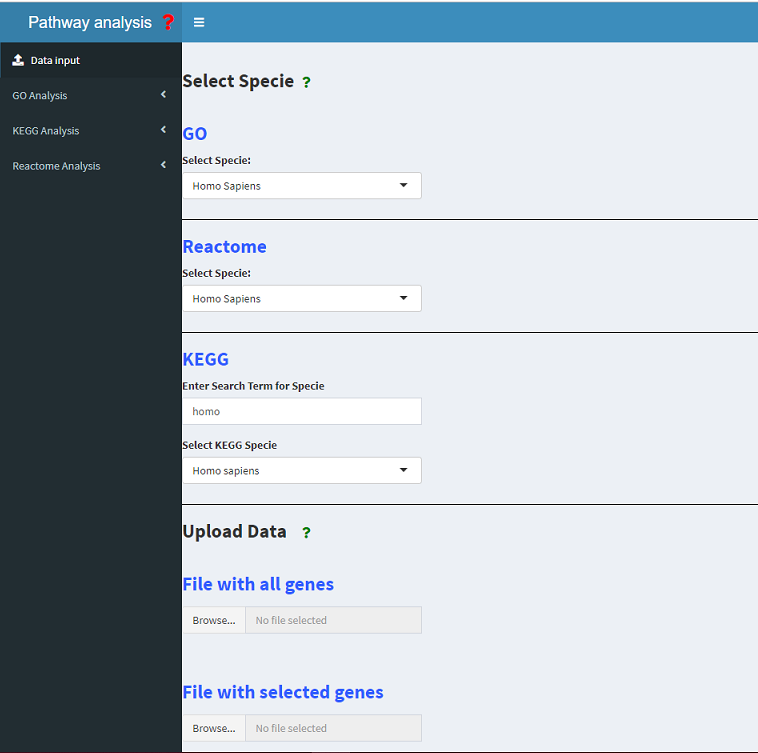
\includegraphics[width=0.9\textwidth]{figures/App_F1.png}
\end{figure}

L'usuari té la possibilitat d'introduir l'arxiu amb tots els gens i els gens seleccionats. Un cop introduïdes les dades es mostra un petit resum del contingut dels arxius.

\begin{figure}[H]
\caption{Resum de les dades pujades}
\centering
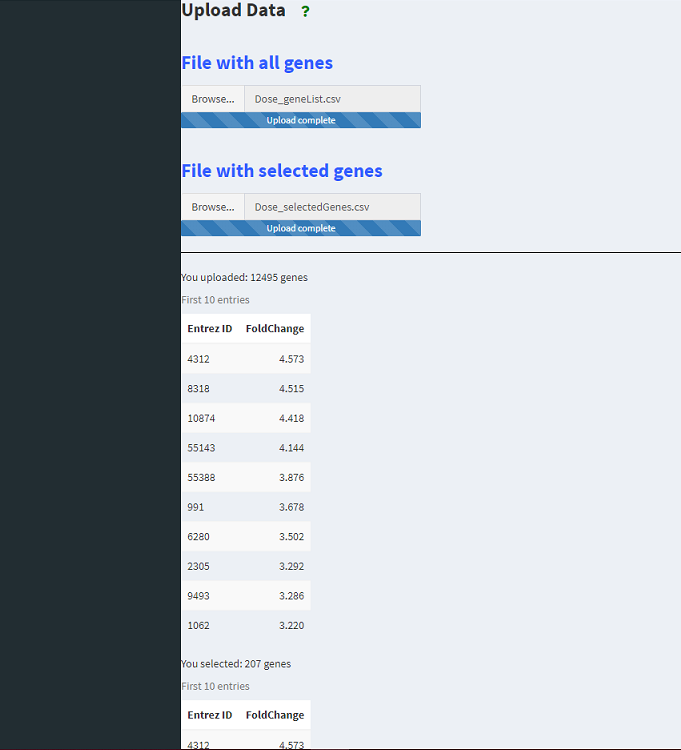
\includegraphics[width=0.9\textwidth]{figures/App_F1b.png}
\end{figure}


L'aplicació està dividida doncs en 4 parts substancials:

\begin{enumerate}
\item Entrada de les dades;
\item Anàlisi GO;
\item Anàlisi KEGG;
\item Anàlisi Reactome.
\end{enumerate}


L'aplicació ofereix dos mètodes d'anàlisi: d'una banda es pot fer \gls{ORA} (Over-Representation Analysis) i d'altra banda l'anàlisi GSEA (Gene Set Enrichment Analisis). Recordem que l'ORA consisteix a seleccionar els gens diferencialment expressats i basant-se en GO, KEGG o Reactome comprovar si una de les agrupacions de gens suggerides per aquestes bases de dades està sobre o sotraexpressada en els gens seleccionats. Per dur a terme l'ORA l'usuari té l’opció de definir un \textit{cut-off} de Log-Ratio per formar el conjunt dels gens que s'hi utilitzarà (\textit{gene set}). \gls{ORA} és una bona eina per veure els efectes grans però els efectes petits se li escapen. Els efectes petits derivats dels gens individuals poden acumular-se en un efecte conjunt substancial el qual \gls{ORA} no serà capaç de detectar. És aquí on GSEA mostra la seva utilitat. 

Els apartats d'anàlisi (GO, KEGG i Reactome) ofereixen tan representacions comunes com representacions específiques. 

Els anàlisis i representacions en comú són:

\begin{itemize}
\item Taula dels resultats ORA;
\item Taula dels resultats GSEA;
\item Gràfic de barres del resultat ORA;
\item Gràfic de punts del resultat ORA;
\item El mapa d'enriquement (Enrichment Map);
\item La xarxa dels gens en categories (Category-gene-network);
\item El gràfic de GSEA.
\end{itemize} 

Les anàlisis específics són:

\begin{itemize}
\item GO $\rightarrow$ Gràfic GO 
\item KEGG $\rightarrow$ Rutes de la base de dades KEGG
\item Reactome $\rightarrow$ Rutes de la base de dades Reactome
\end{itemize}

\begin{figure}[H]
\centering
\begin{tabular}{ccc}
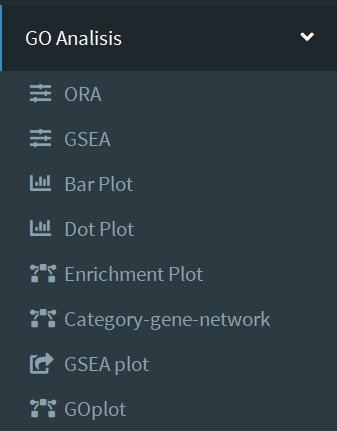
\includegraphics[width=45mm]{figures/App_F2_Items_GO.png} & 
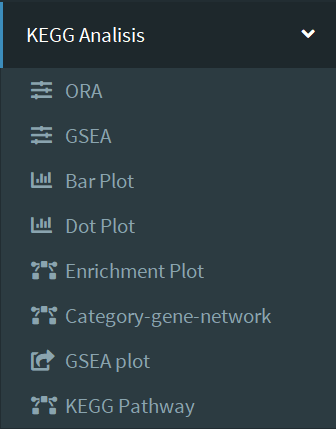
\includegraphics[width=45mm]{figures/App_F3_Items_KEGG.png} &
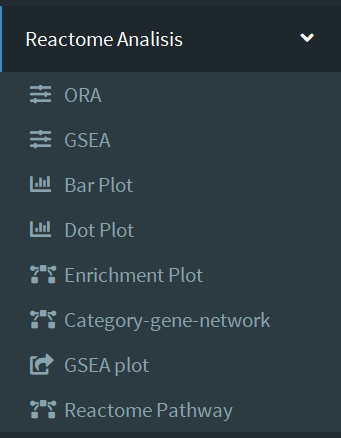
\includegraphics[width=45mm]{figures/App_F4_Items_RA.png} \\
(a) GO & (b) KEGG & (c) Reactome \\
\end{tabular}
\caption{Els elements de les seccions d'anàlisi}
\end{figure}


\label{sec:ACom}

\section{ORA}

\subsection{GO}

Per realitzar l'anàlisi \gls{ORA} per a termes GO s'utilitza la funció \helvetica{enrichGO} del paquet \helvetica{clusterPrifiler}.

He implementat els valors per defecte amb la possibilitat per a l’usuari d'elegir entre:

\begin{itemize}
\item \underline{Ontologies GO} 
\begin{itemize}
\item Molecular function, Biological proces, Cellular Components;
\end{itemize}
\item \underline{Nivell de significació basant-se en els valors de P ajustats}
\begin{itemize}
\item 0.1, 0.05, 0.01, 0.001;
\end{itemize}
\item \underline{Mètode d'ajustament}
\begin{itemize}
\item Holm; Hochberg; Hommel; Bonferroni; BH; BY; FDR; None.
\end{itemize}
\end{itemize}

\begin{figure}[h!]
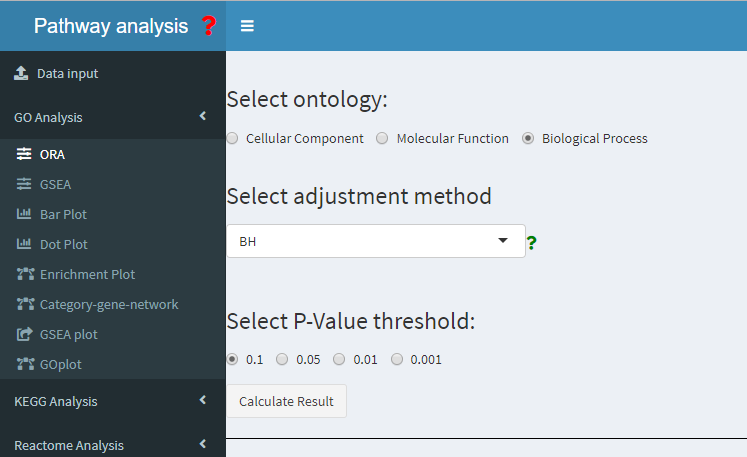
\includegraphics[width=0.9\textwidth]{figures/App_F5_Items_GO_ORA.png}
\caption{Especificació d'ORA dels termes GO}
\end{figure}
L'execució de la funció és un procès temporalment costós. Per aquest motiu he afegit el botó d'acció, en lloc de deixar la funció reactiva. D'aquesta manera l'usuari ha de fer una decisió conscient de repetir l'anàlisi amb altres valors.

Prement el botó apareix la taula i el botó nou mitjançant el qual l'usuari pot descarregar els resultats en format .csv. He formatejat la taula amb els paquets \helvetica{knitr}, \helvetica{kableExtra}, \helvetica{formattable} i \helvetica{dplyr}. Amb els dos últims he afegit les barres de color pel nombre dels gens diferencialment expressats del terme específic de GO i la gradació de color del verd fins al vermell pels valors dels més petits fins els més grans. 

\begin{figure}[h!]
\centering
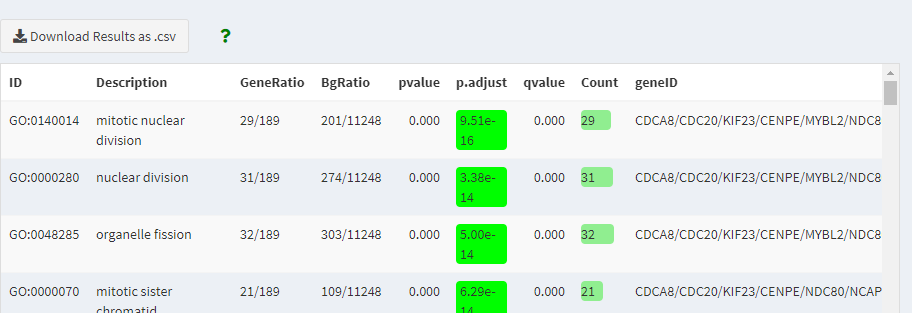
\includegraphics[width=0.9\textwidth]{figures/App_F6_Items_GO_ORA_Table.png} 
\caption{El resultat d'anàlisi ORA. GO.}
\end{figure}


\subsection{KEGG}

Per l'ORA de base de dades KEGG he utilitzat la funció \helvetica{enrichKEGG()} del paquet \helvetica{clusterProfiler}. 



\begin{figure}[H]
\centering
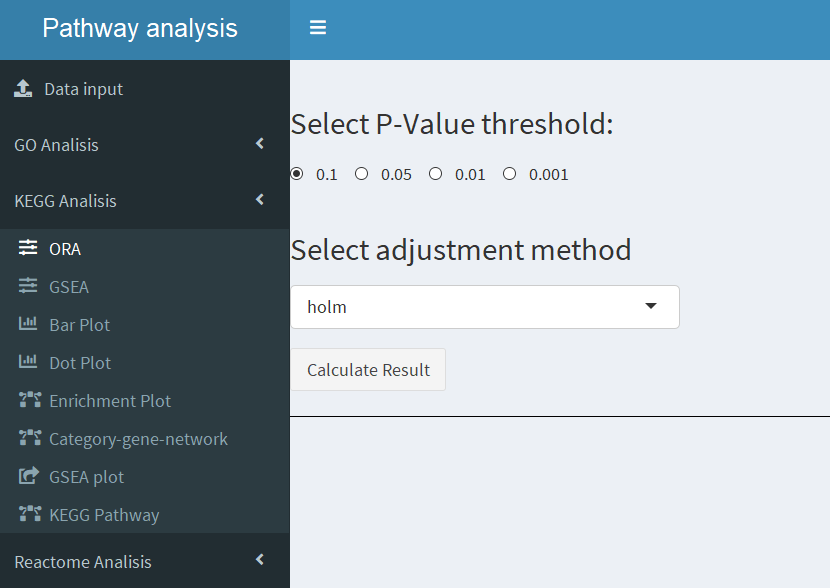
\includegraphics[width=0.9\textwidth]{figures/App_F7_Items_KEGG_ORA.png} 
\caption{Configuració d'anàlisi KEGG}
\end{figure}



Una vegada introduïts els paràmetres i premut el botó \textbf{Calculate} apareix el botó \textbf{Download .csv} i la taula previsualitzada. Els camps de la taula són els mateixos com en l'anàlisi dels termes GO.
\begin{figure}[H]
\centering
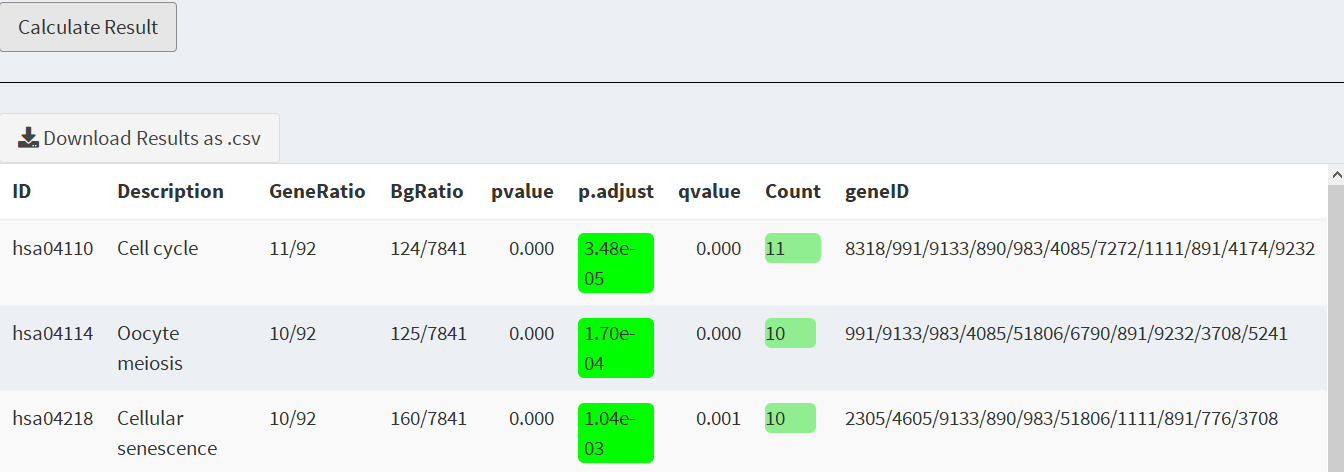
\includegraphics[width=0.9\textwidth]{figures/App_F9_Items_KEGG_ORA_Table.png} 
\caption{El resultat de l'anàlisi ORA. KEGG.}
\end{figure}

\subsection{Reactome}
En el cas de Reactome el procediment és similar. La funció usada és \helvetica{enrichPathway()} del paquet \helvetica{ReactomePA}:


\begin{figure}[H]
\centering
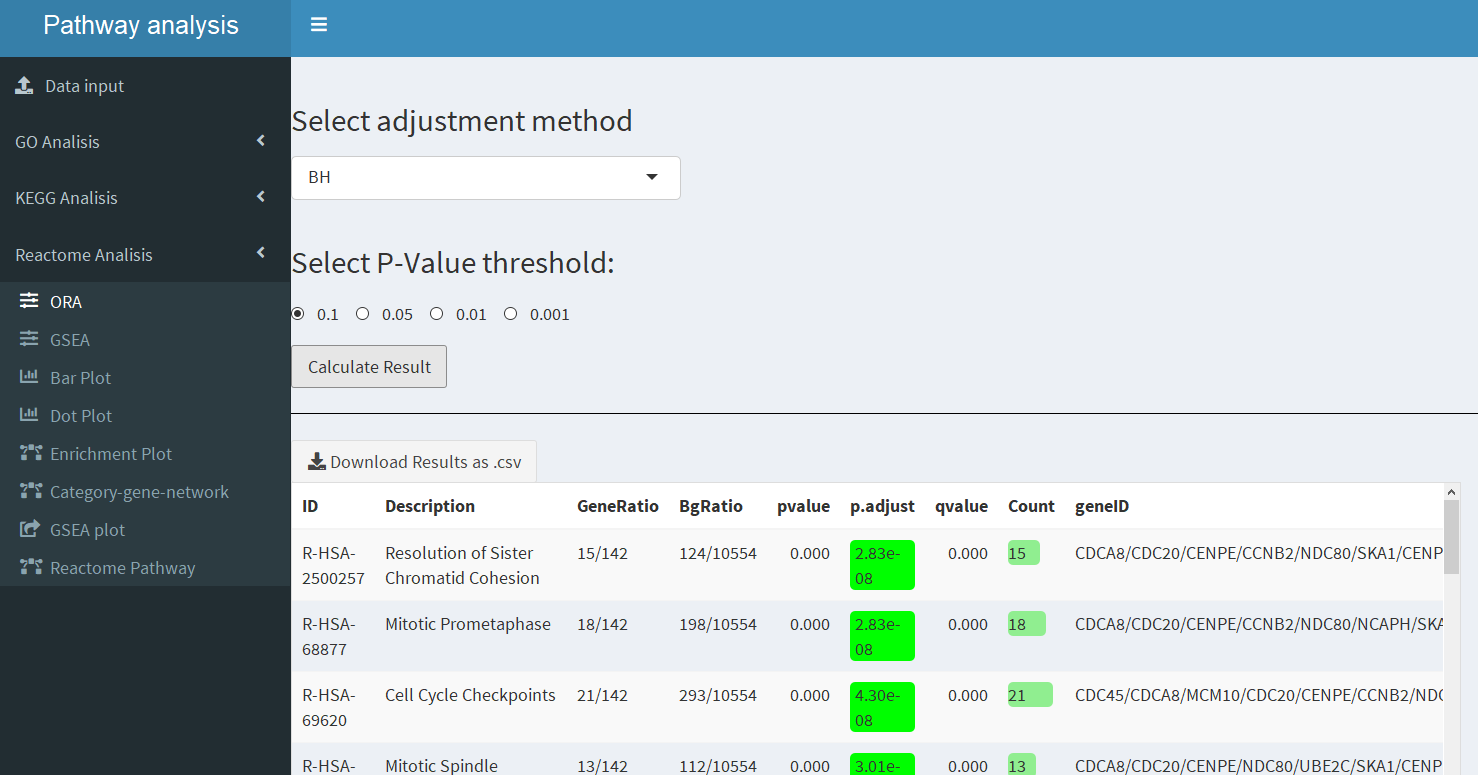
\includegraphics[width=0.9\textwidth]{figures/App_F10_Items_Reactome_ORA.png} 
\caption{El resultat d'anàlisi ORA. Reactome.}
\end{figure}

\section{GSEA}
\subsection{GO}
El mètode GSEA per a termes GO es calcula amb la funció \helvetica{gseGO()} del paquet \helvetica{clusterProfiler}. 

L'usuari pot elegir l'ontologia GO, el \textit{cut-off} del valor P i el mètode d'ajustament.
\begin{figure}[H]
\centering
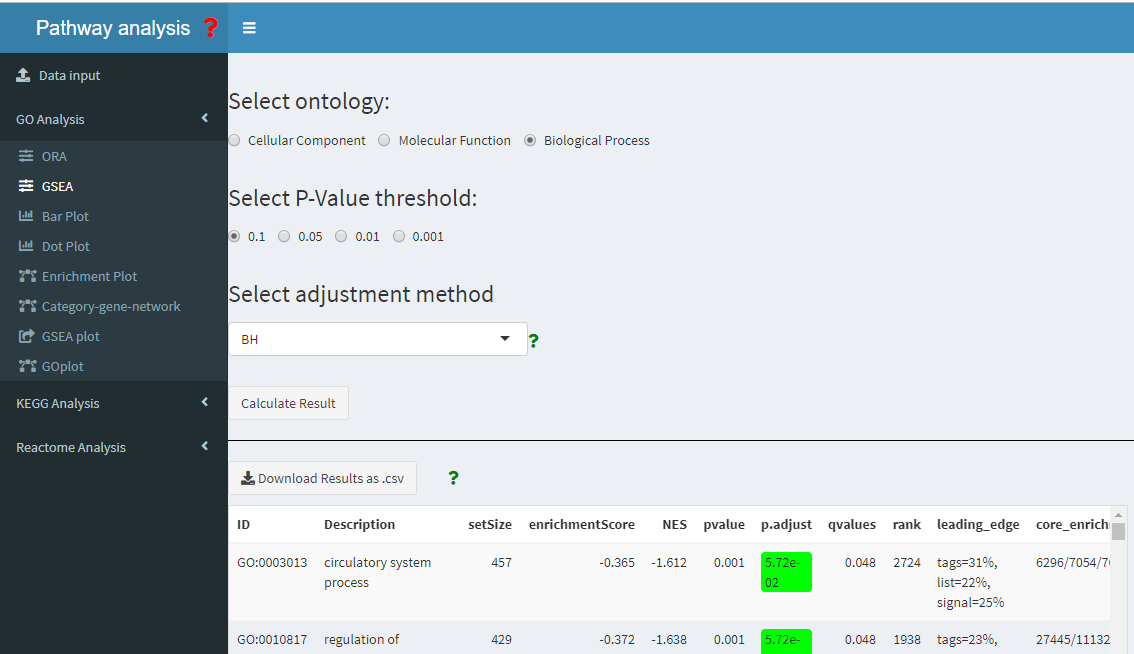
\includegraphics[width=0.9\textwidth]{figures/App_F11_Items_GO_GSEA.png} 
\caption{El resultat de l'anàlisi GSEA. GO.}
\end{figure}


\subsection{KEGG}
De la mateixa manera es calcula GSEA amb la funció \helvetica{gseKEGG()} del paquet \helvetica{clusterProfiler}:

\begin{figure}[H]
\centering
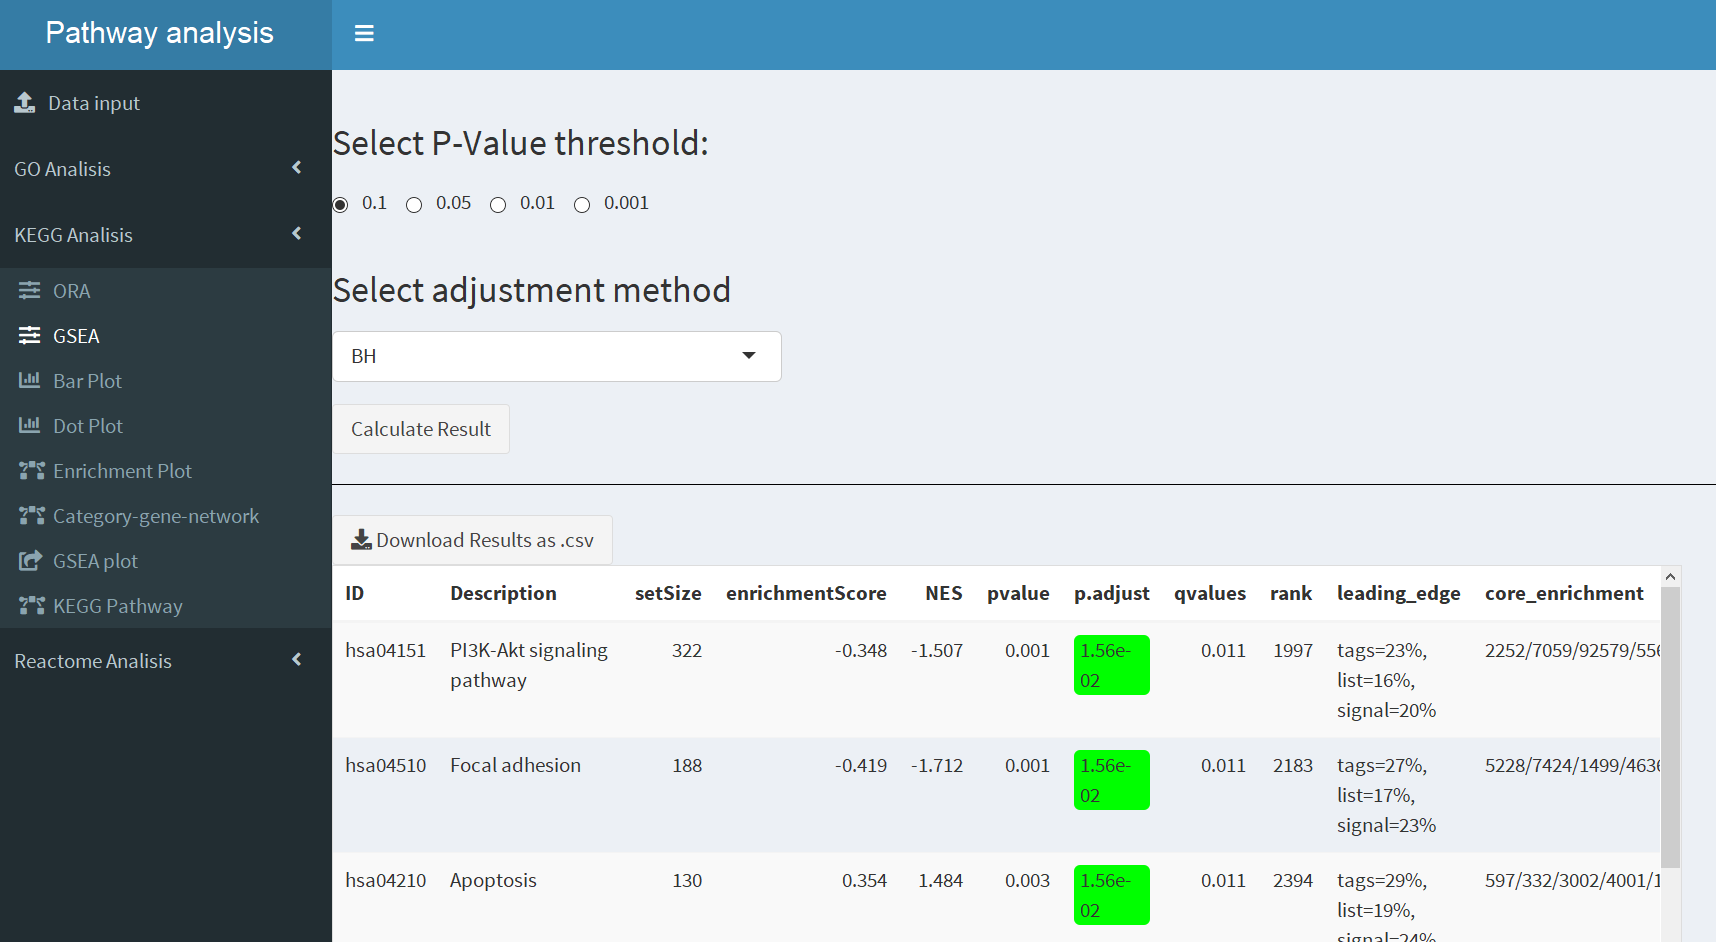
\includegraphics[width=0.9\textwidth]{figures/App_F12_Items_KEGG_GSEA.png} 
\caption{El resultat de l'anàlisi GSEA. KEGG.}
\end{figure}

\subsection{Reactome}
Per completar l'anàlisi l'usuari pot calcular GSEA per a base de dades Reactome. Com als altres casos utilitzo el paquet \helvetica{clusterProfiler} i específicament la funció \helvetica{gsePathway()}

\begin{figure}[H]
\centering
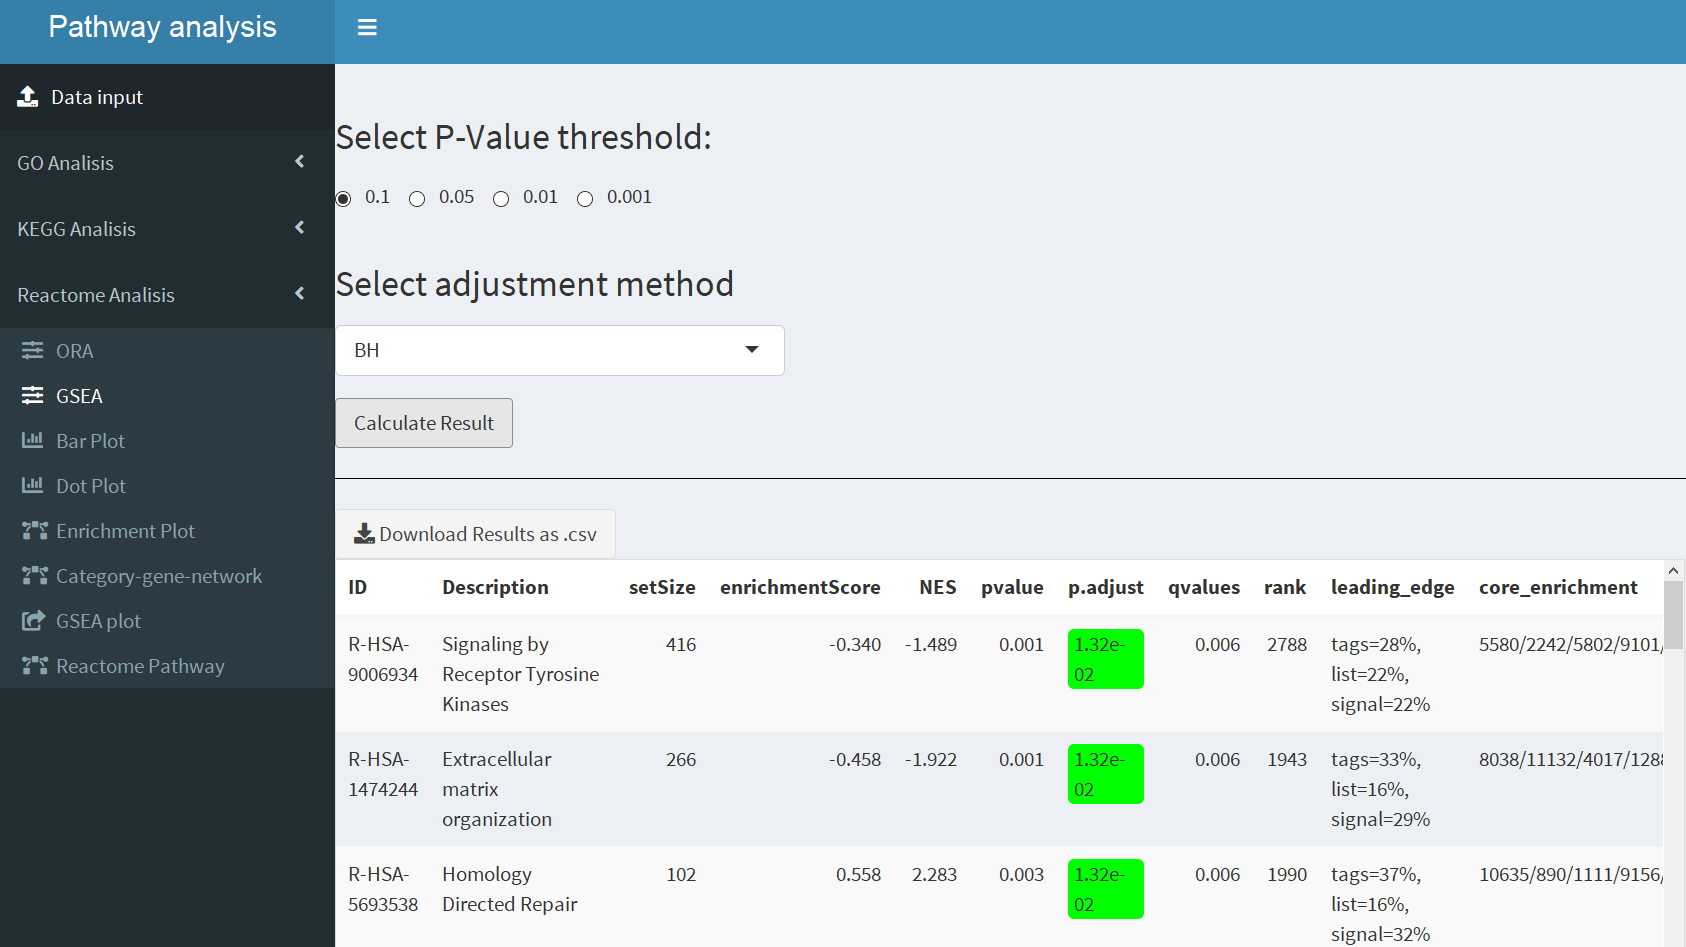
\includegraphics[width=0.9\textwidth]{figures/App_F13_Items_RA_GSEA.png} 
\caption{El resultat d'anàlisi GSEA. Reactome.}
\end{figure}

\section{Visualització i l'anàlisi topològic}

\subsection{Bar-Plots}
Els resultats de \helvetica{enrichGO}, \helvetica{enrichKEGG} i \helvetica{enrichPathway} es poden visualitzar amb el gràfic de barres. L'usuari pot elegir el nombre de les categories visualitzades entre 2 i 30. Es dona l'opció per descarregar el gràfic en format .png.

\begin{figure}[H]
\centering
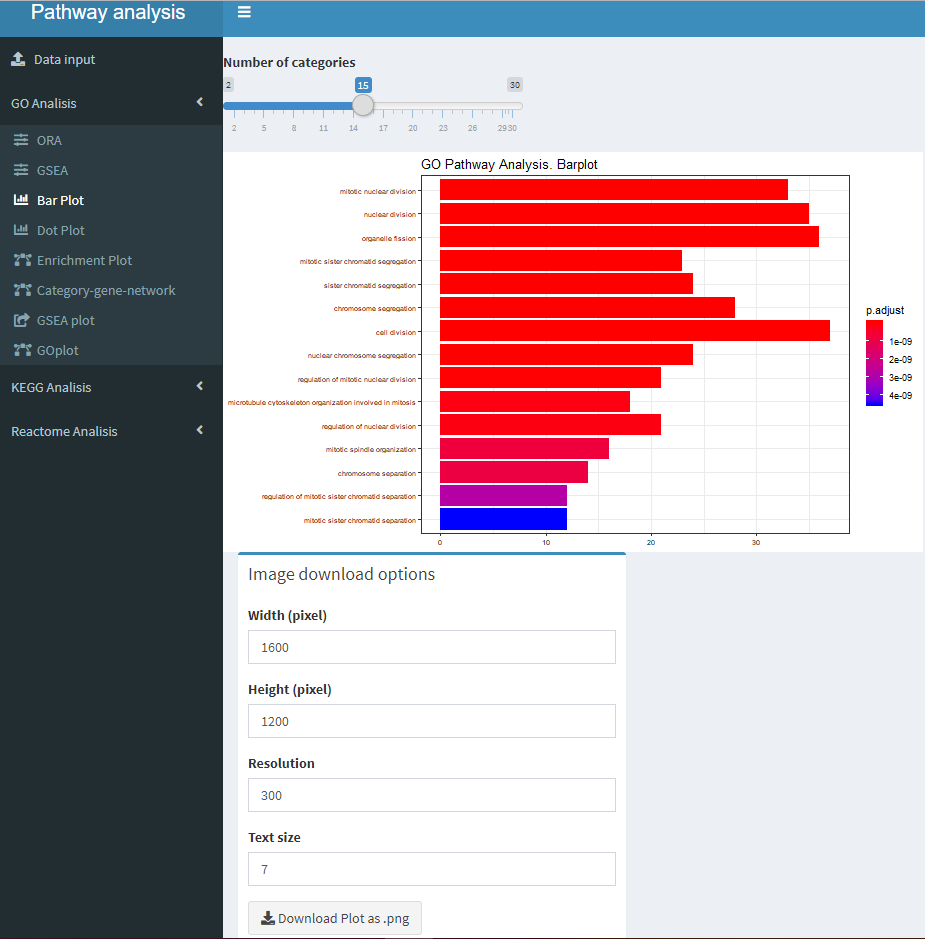
\includegraphics[width=0.9\textwidth]{figures/App_F14_Items_GO_BarPlot.png} 
\caption{Bar-Plot. GO.}
\end{figure}

\subsection{Dot-Plots}

El \textit{dot plot} visualitza addicionalment el \textit{gen ratio}. També aquí l'usuari pot seleccionar el nombre de categories.


\begin{figure}[H]
\centering
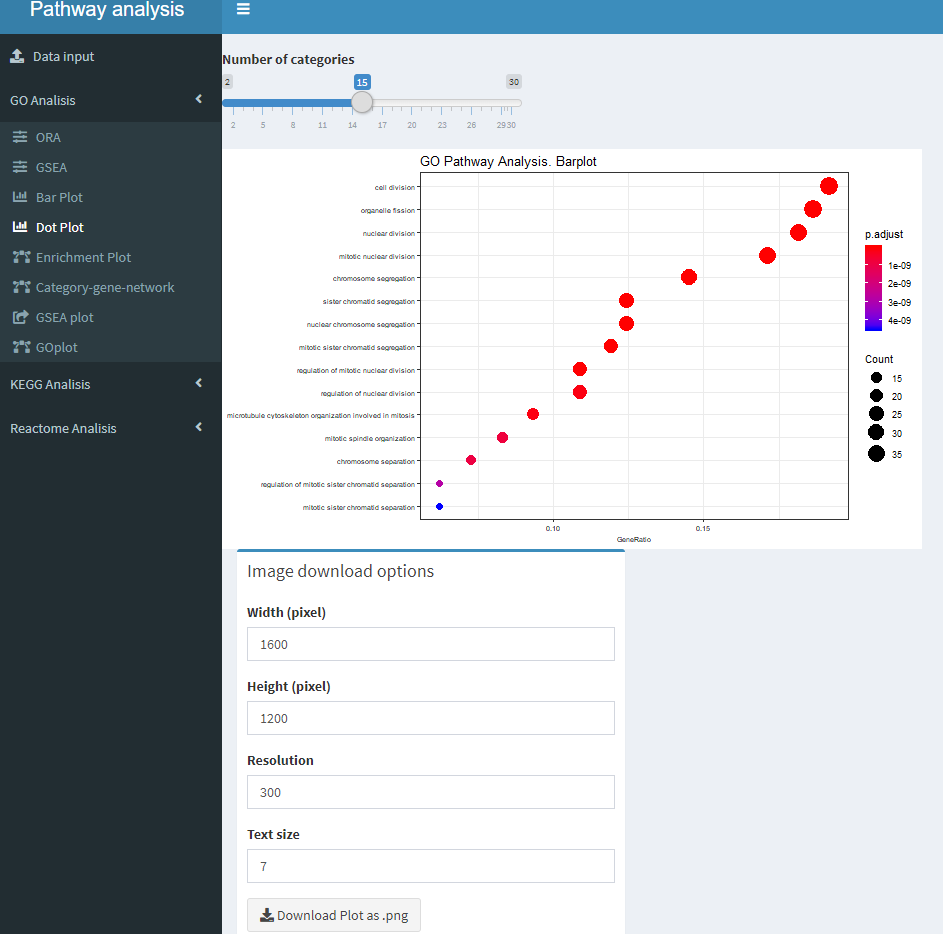
\includegraphics[width=0.9\textwidth]{figures/App_F15_Items_GO_DotPlot.png} 
\caption{Bar-Plot. GO.}
\end{figure}

\subsection{Enrichment Plots}

\begin{figure}[H]
\centering
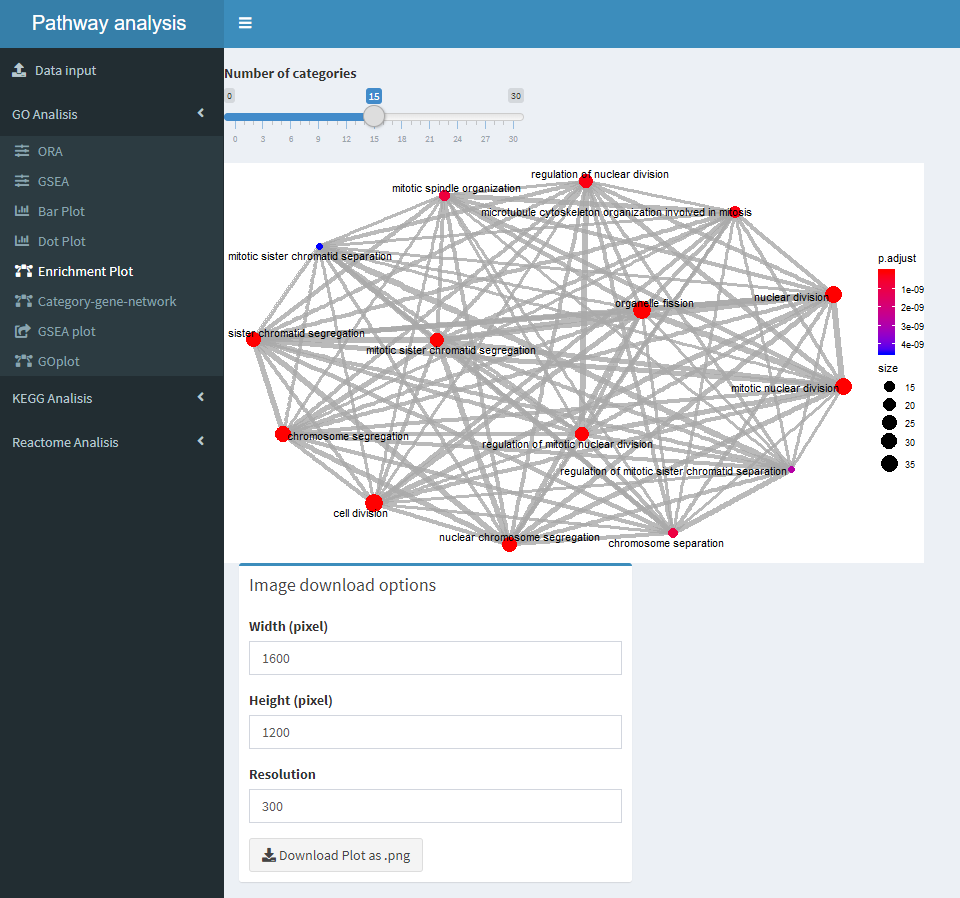
\includegraphics[width=0.9\textwidth]{figures/App_F16_Items_GO_Emap.png} 
\caption{Bar-Plot. GO.}
\end{figure}

\subsection{Category-Gene-Network Plot}

\begin{figure}[H]
\centering
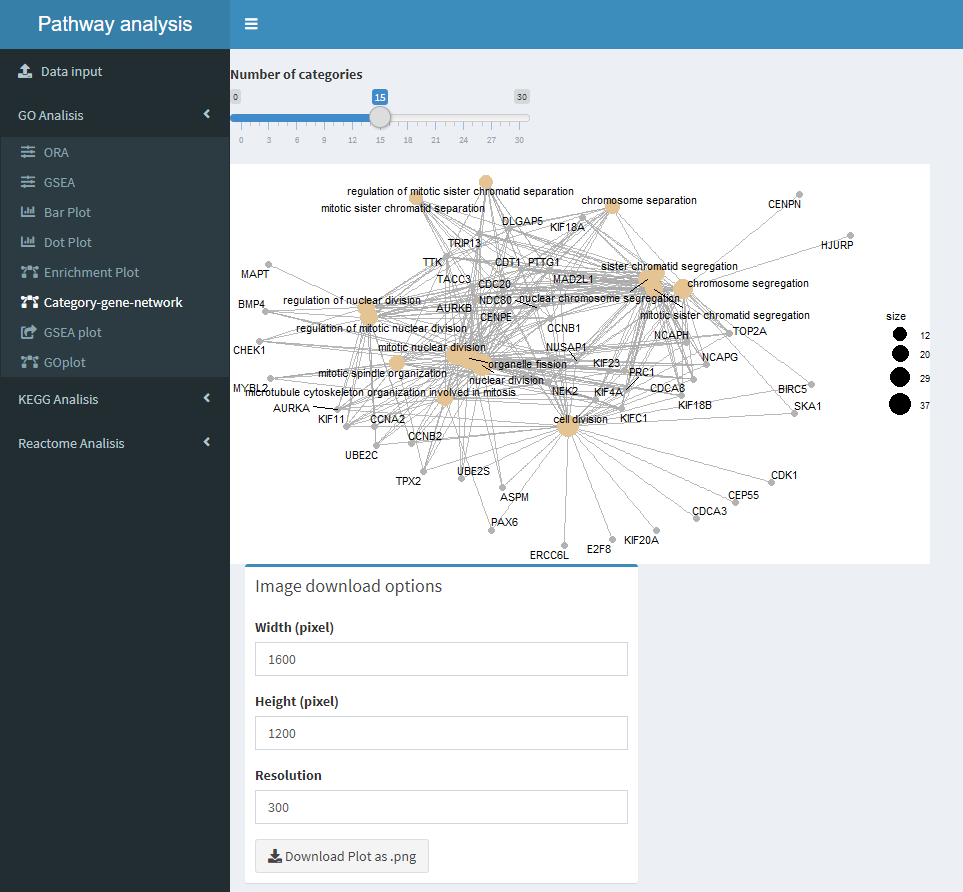
\includegraphics[width=0.9\textwidth]{figures/App_F17_Items_GO_CnetPlot.png} 
\caption{Category-Gene-Network Plot. GO.}
\end{figure}

\subsection{GSEA Plot}
L'usuari pot visualitzar una de les categories disponibles via \textit{dropdown list}. El llistat inclou totes les rutes generades durant l'anàlisi GSEA en els apartats \textit{Go Analysis}$\rightarrow$\textit{GSEA}; \textit{KEGG}$\rightarrow$\textit{GSEA}
\begin{figure}[H]
\centering
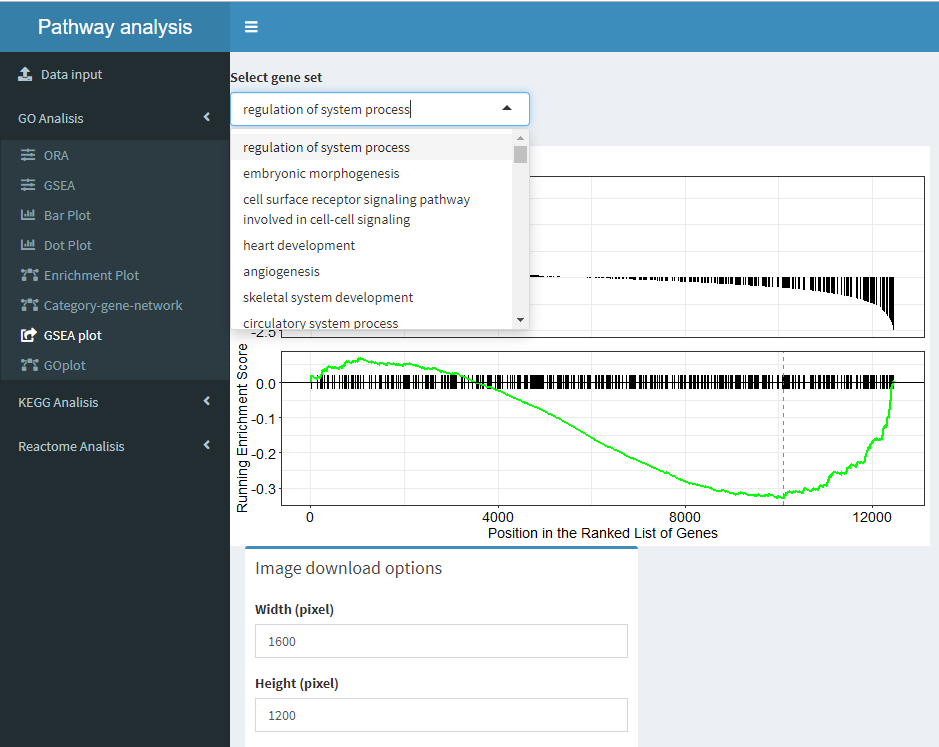
\includegraphics[width=0.9\textwidth]{figures/App_F18_Items_GO_GSEA_Plot.png} 
\caption{GSEA Plot. GO.}
\end{figure}


\subsection{GO Plot}

\begin{figure}[H]
\centering
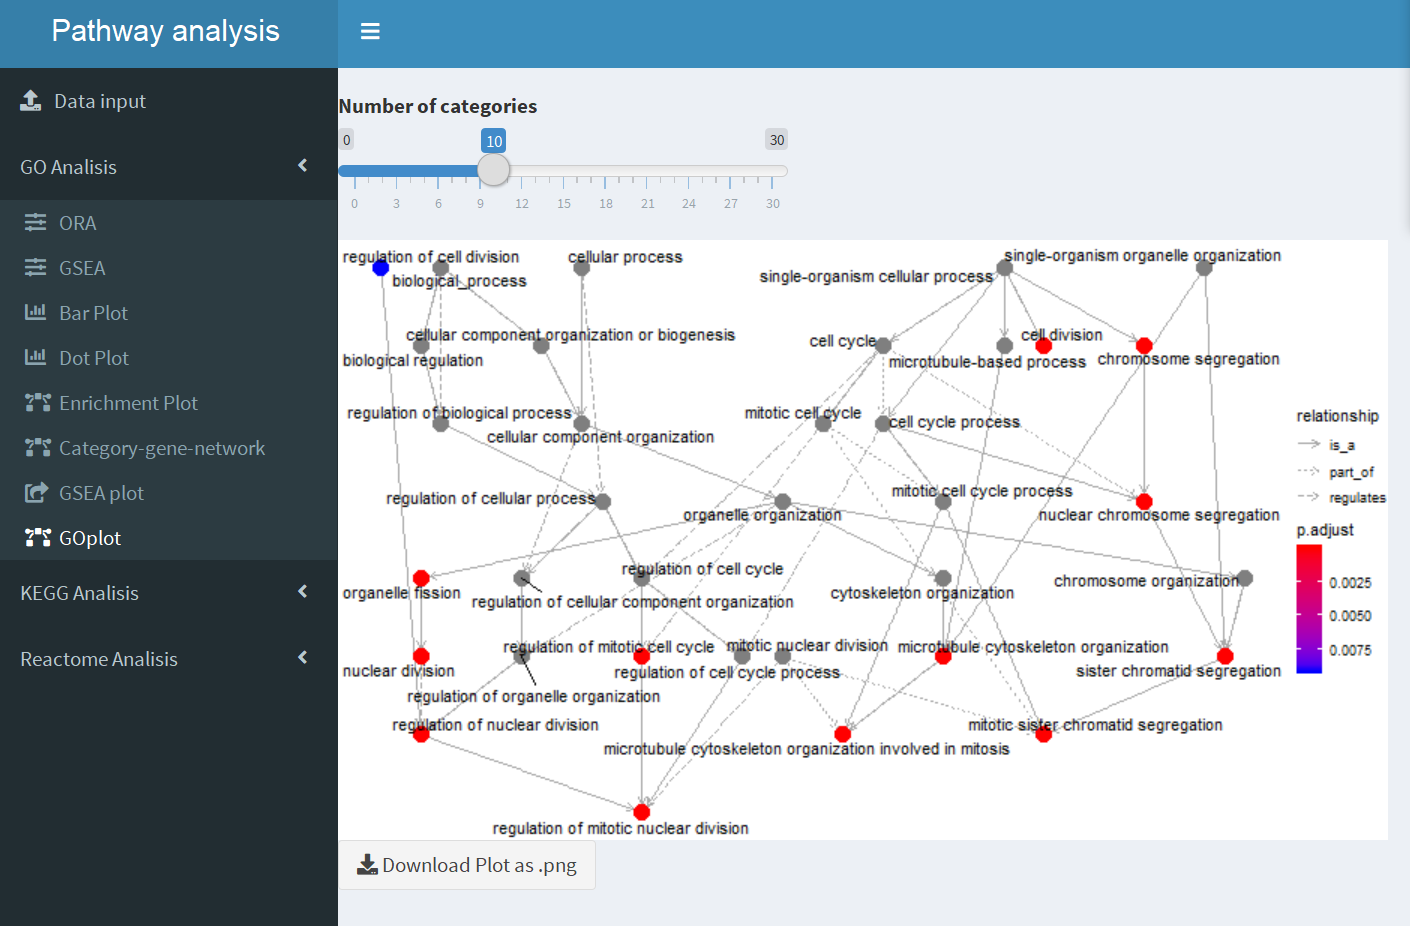
\includegraphics[width=0.9\textwidth]{figures/App_F19_Items_GO_GOPlot.png} 
\caption{GO Plot}
\end{figure}

\subsection{KEGG Pathway}


\begin{figure}[H]
\centering
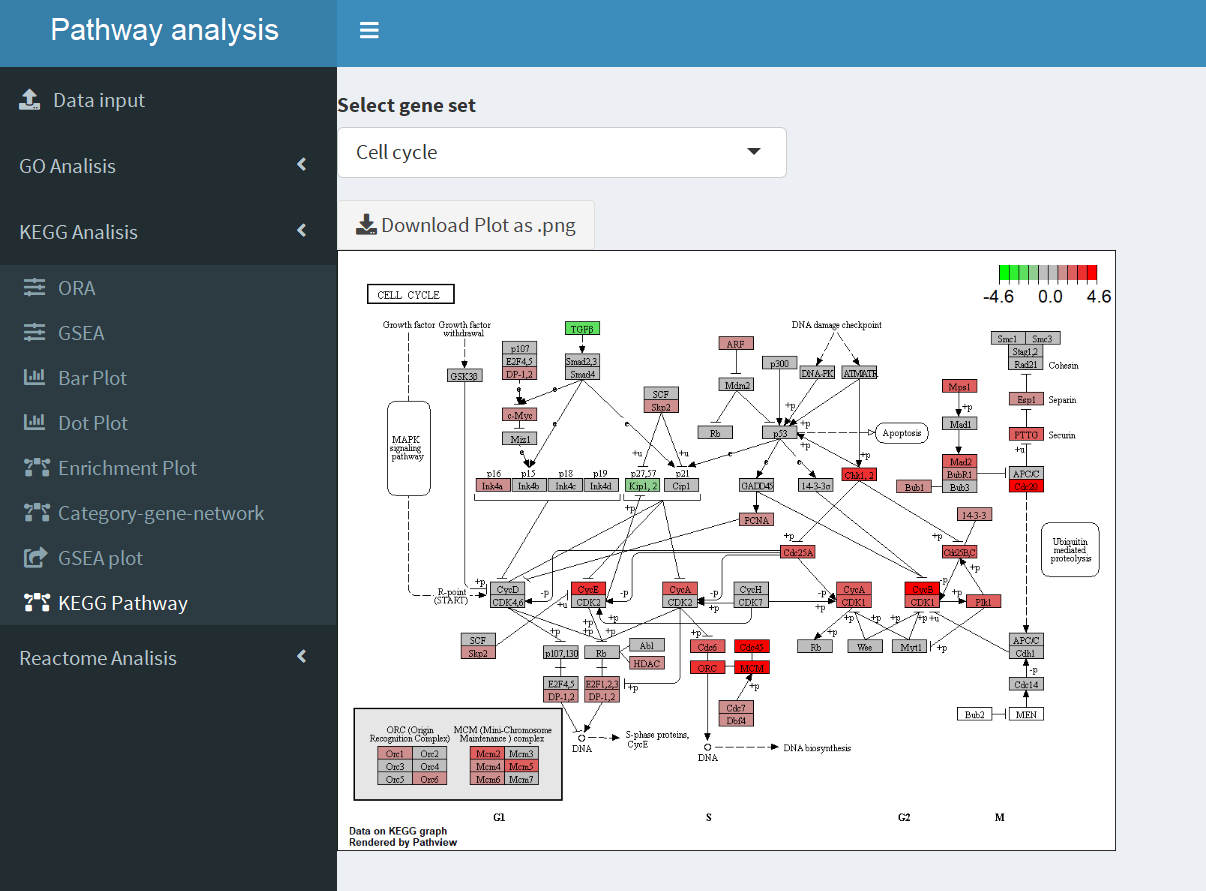
\includegraphics[width=0.9\textwidth]{figures/App_F20_Items_KEGG_KEGGPathway.png} 
\caption{KEGG pathway}
\end{figure}

\subsection{Reactome Pathway}

\begin{figure}[H]
\centering
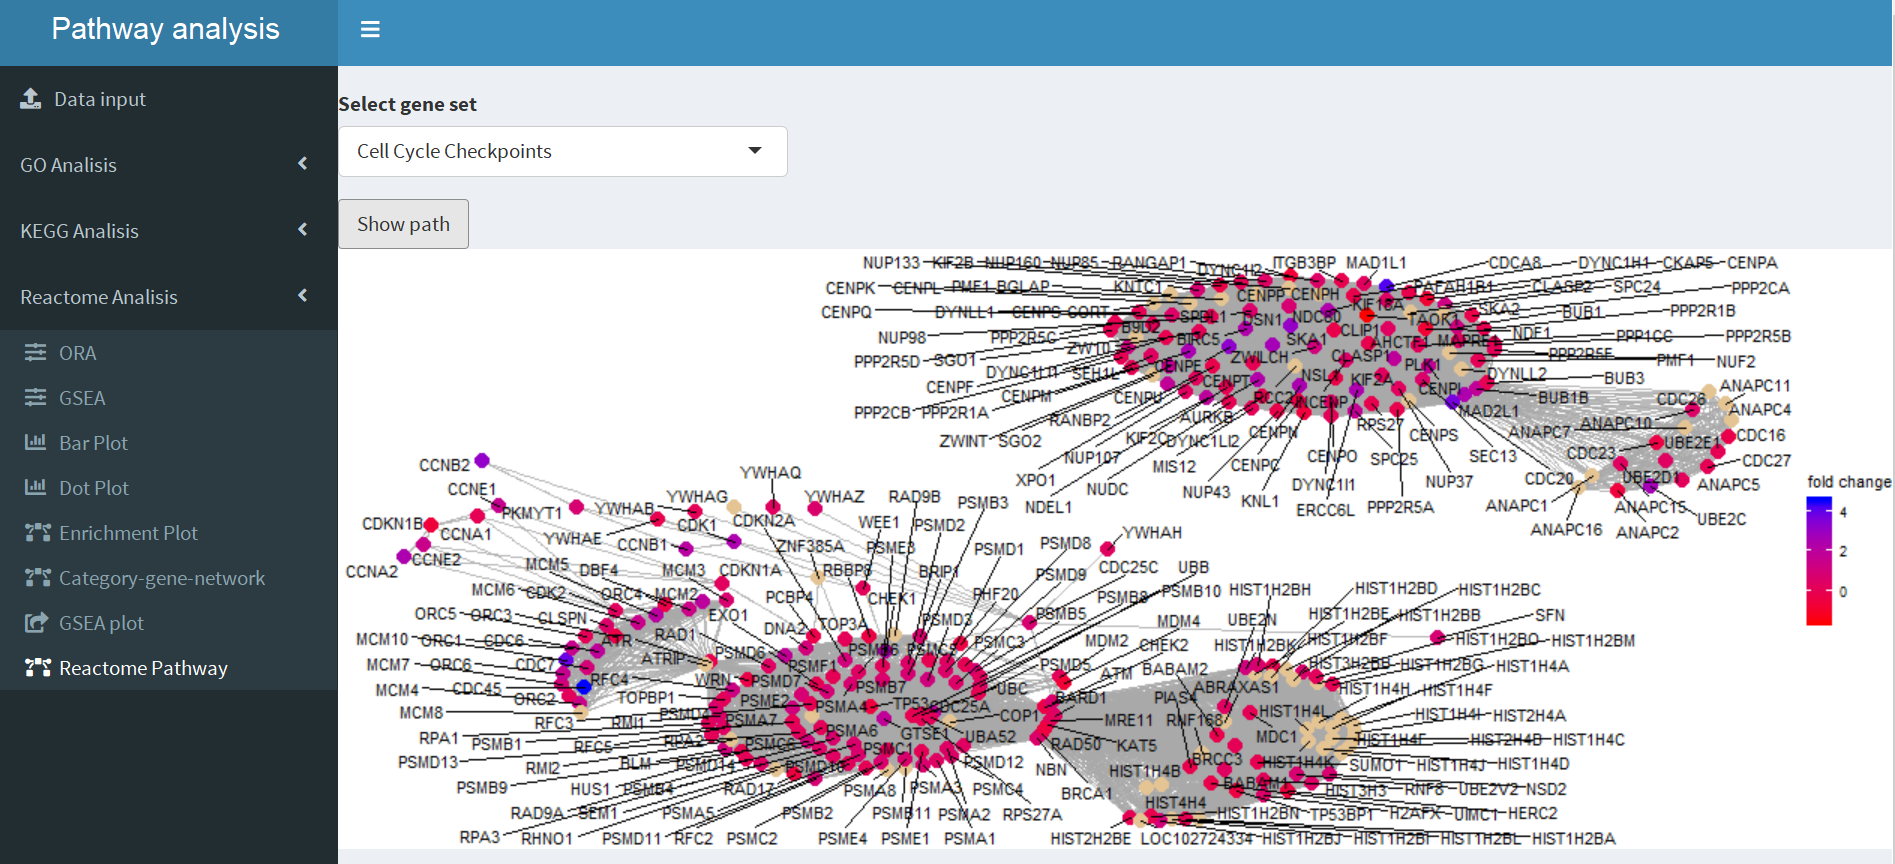
\includegraphics[width=0.9\textwidth]{figures/App_F21_Items_RA_RAPathway.png} 
\caption{Reactome pathway}
\end{figure}


\section{Manual i les ajudes del programa}

Per facilitar l'ús de l’aplicació he pensat com es podria fer de manera més intuïtiva possible. Primer cal destacar que com a llengua de manual he elegit l’anglès per poder fer l'ús de l'aplicació el més inclusiu possible. Segon, l'usuari pot accedir tant al manual com a l'ajuda, que es guarden en arxius .Md separats. Per accedir al manual l'usuari ha de clicar al símbol d’interrogació a prop del títol \textbf{Pathway analysis}:
\begin{figure}[H]
\centering
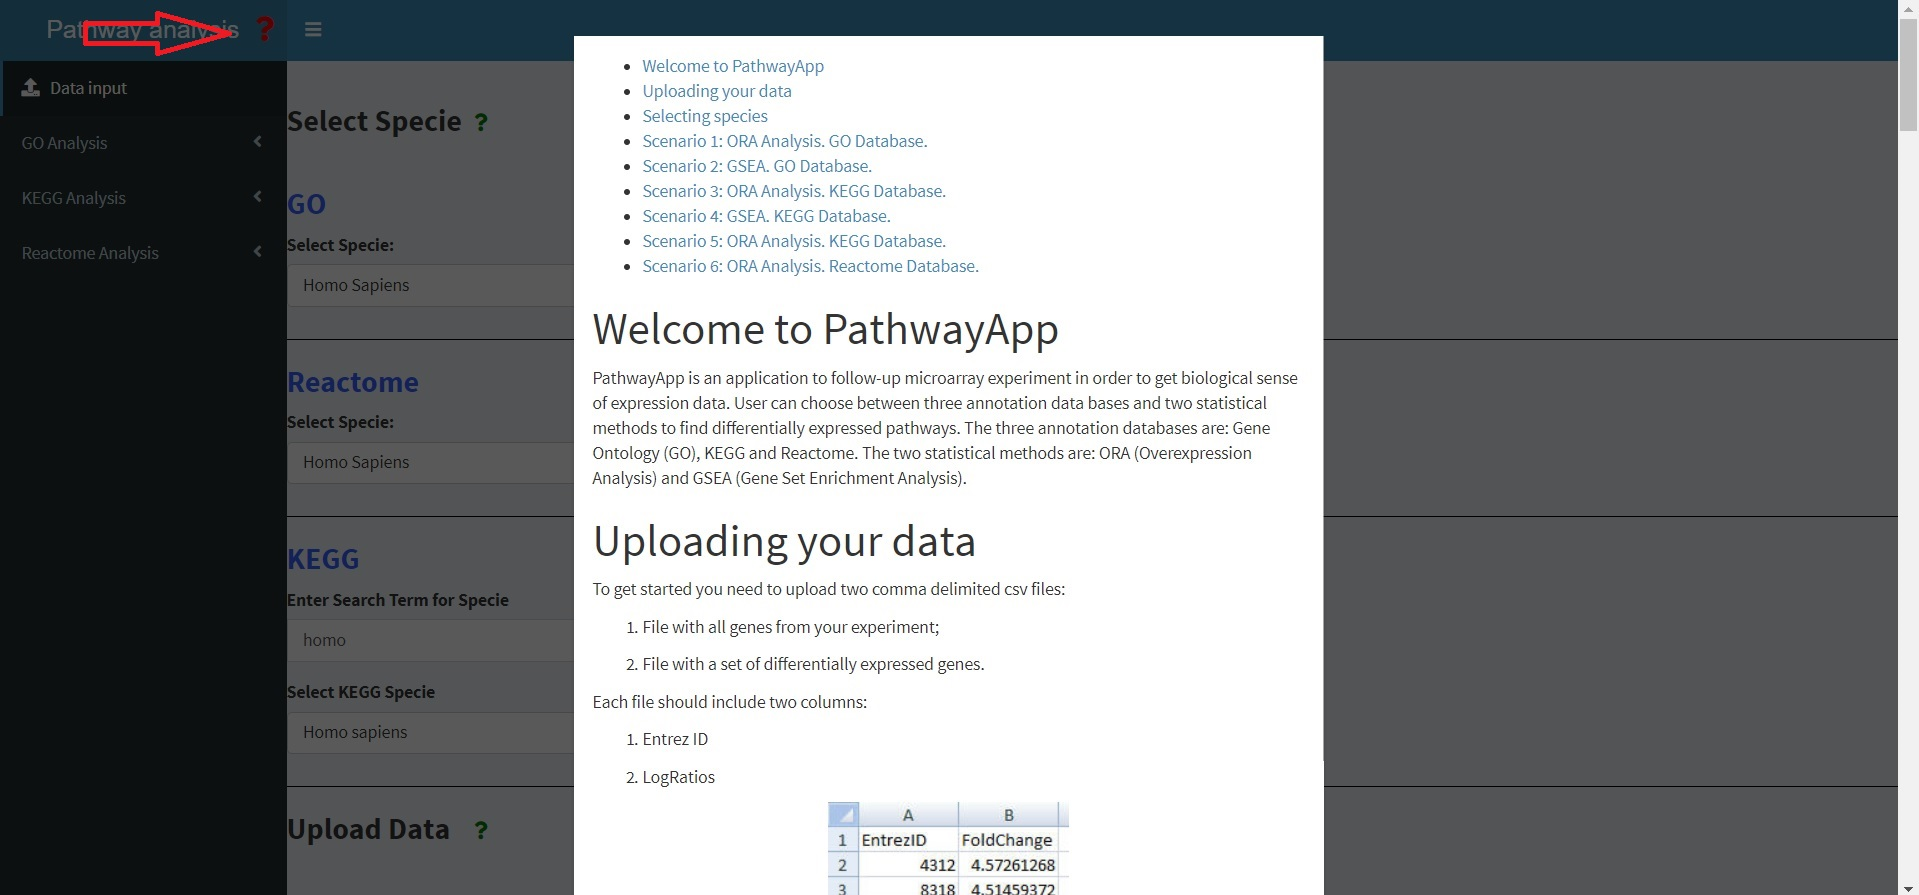
\includegraphics[width=1\textwidth]{figures/Manual.jpg} 
\caption{Manual per a aplicació}
\end{figure}

Com es veu hi ha apartats diferents. Depenent dels objectius de l'usuari, aquest pot seleccionar l'apartat que més l'interessi. Així, si l'usuari vol fer l'anàlisi \gls{ORA} amb l'anotació KEGG pot navegar en la secció |textbf{Scenario 3: \gls{ORA} Analysis. KEGG Database}. 

\begin{figure}[H]
\centering
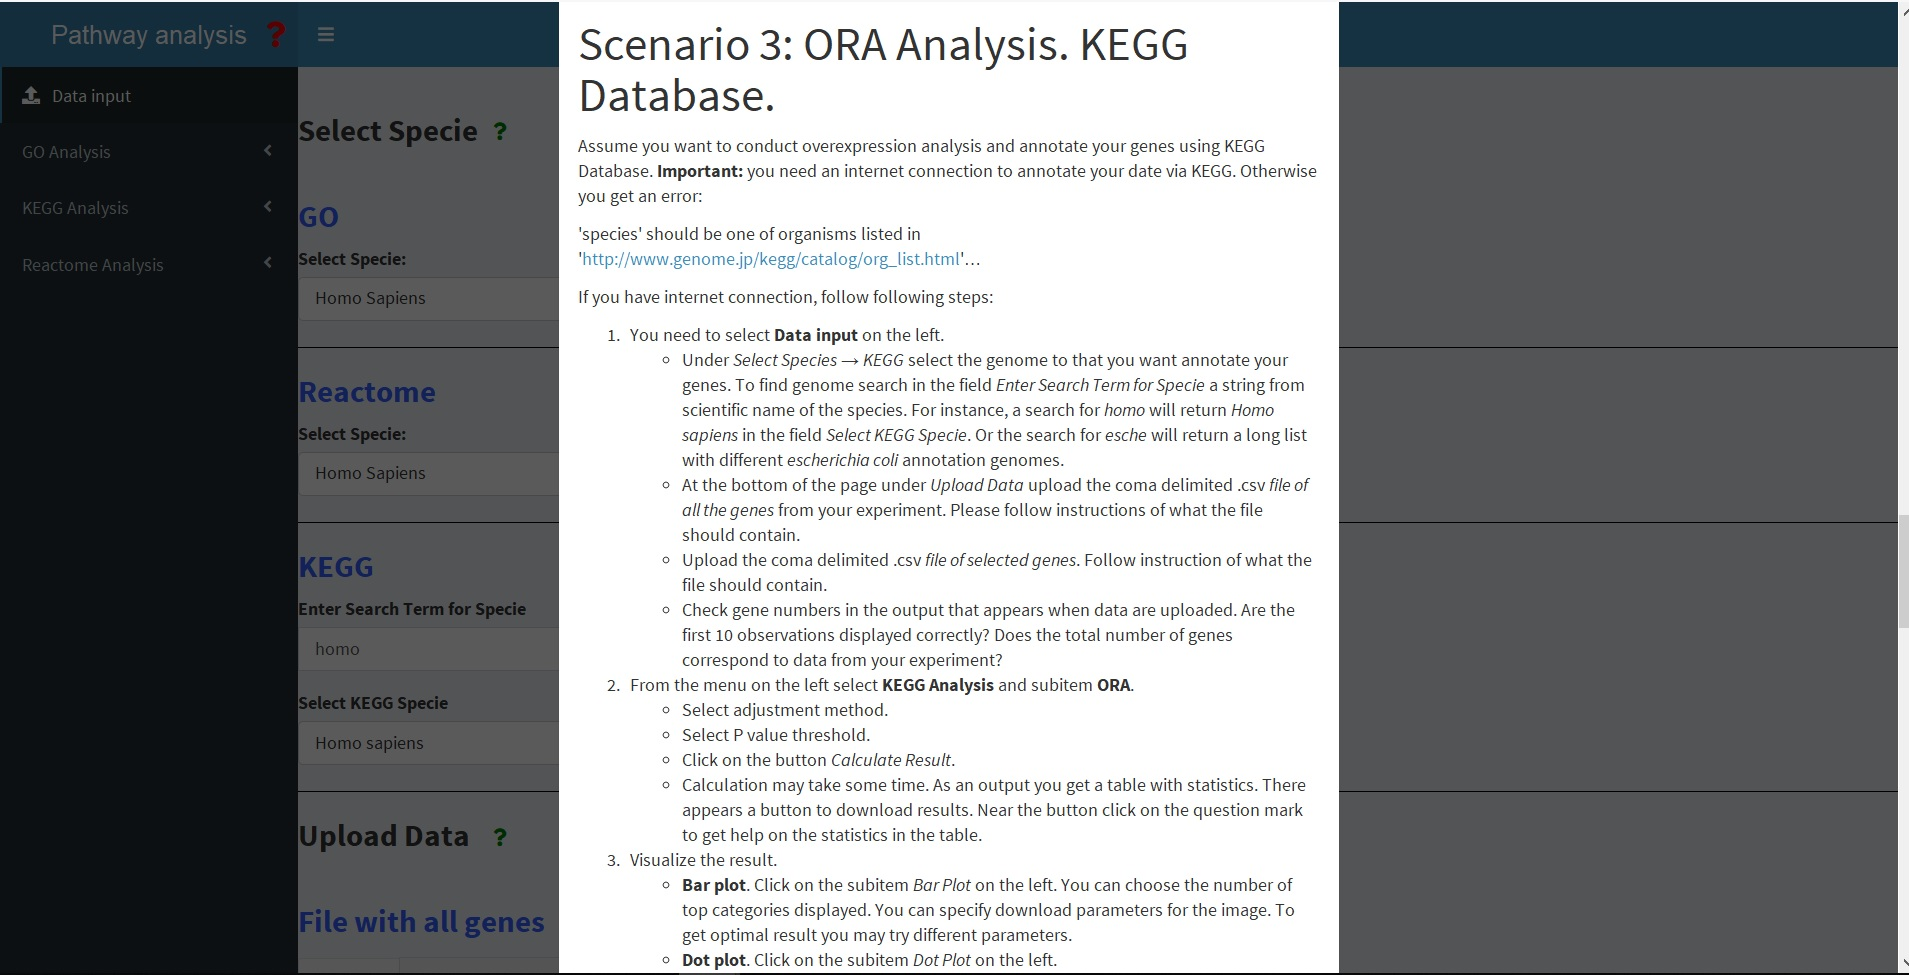
\includegraphics[width=1\textwidth]{figures/Manual2.jpg} 
\caption{Manual per a l'anàlisi \gls{ORA} amb l'anotació KEGG}
\end{figure}


També, l'usuari pot accedir a l'ajuda clicant als símbols d'interrogació distribuïts per l’aplicació en els llocs que penso que poden generar dubtes. 

Per fer-ho possible s'utilitza el paquet \helvetica{shinyhelper} que s'instal·la en executar la funció \helvetica{runPathwayApp()}.

\begin{figure}[H]
\centering
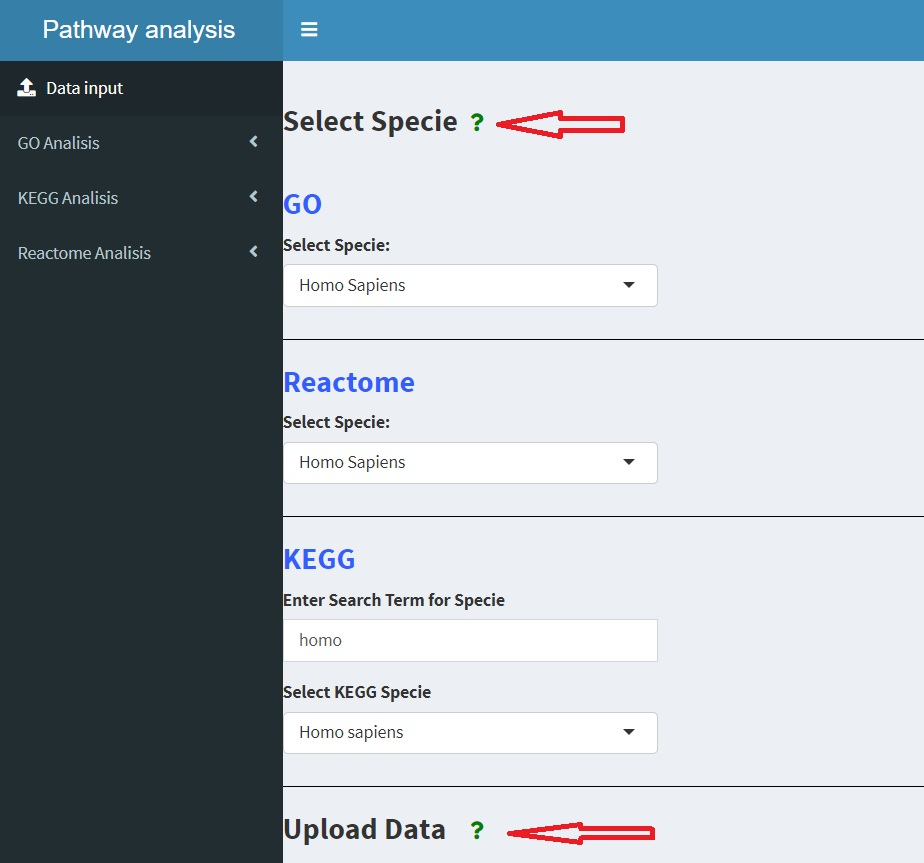
\includegraphics[width=0.7\textwidth]{figures/Help_Data_Input.jpg} 
\caption{Senyals d'ajuda}
\end{figure}

El clic en aquests senyals fa que aparegui una finestreta amb la informació d'ajuda.

Aquí hi ha informació de l'apartat \textbf{Data Input}:

\begin{figure}[H]
\centering
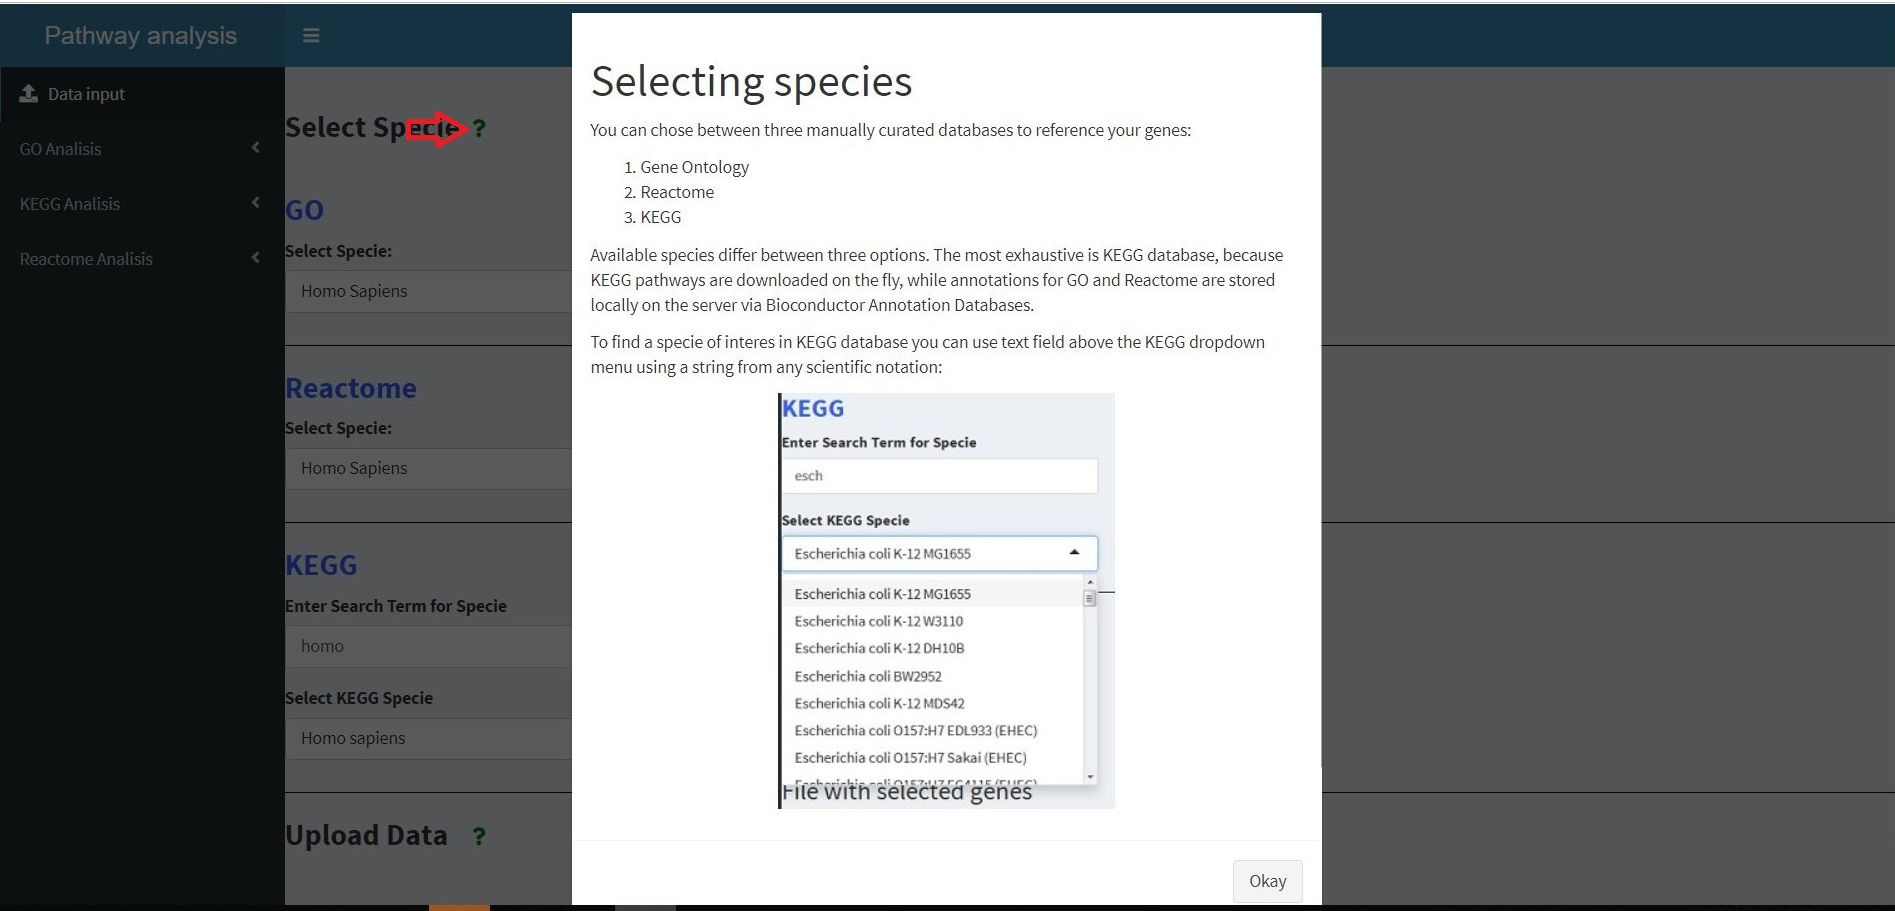
\includegraphics[width=0.9\textwidth]{figures/Help_Specie.jpg} 
\caption{Ajuda per a l'elecció de l'espècie}
\end{figure}

\begin{figure}[H]
\centering
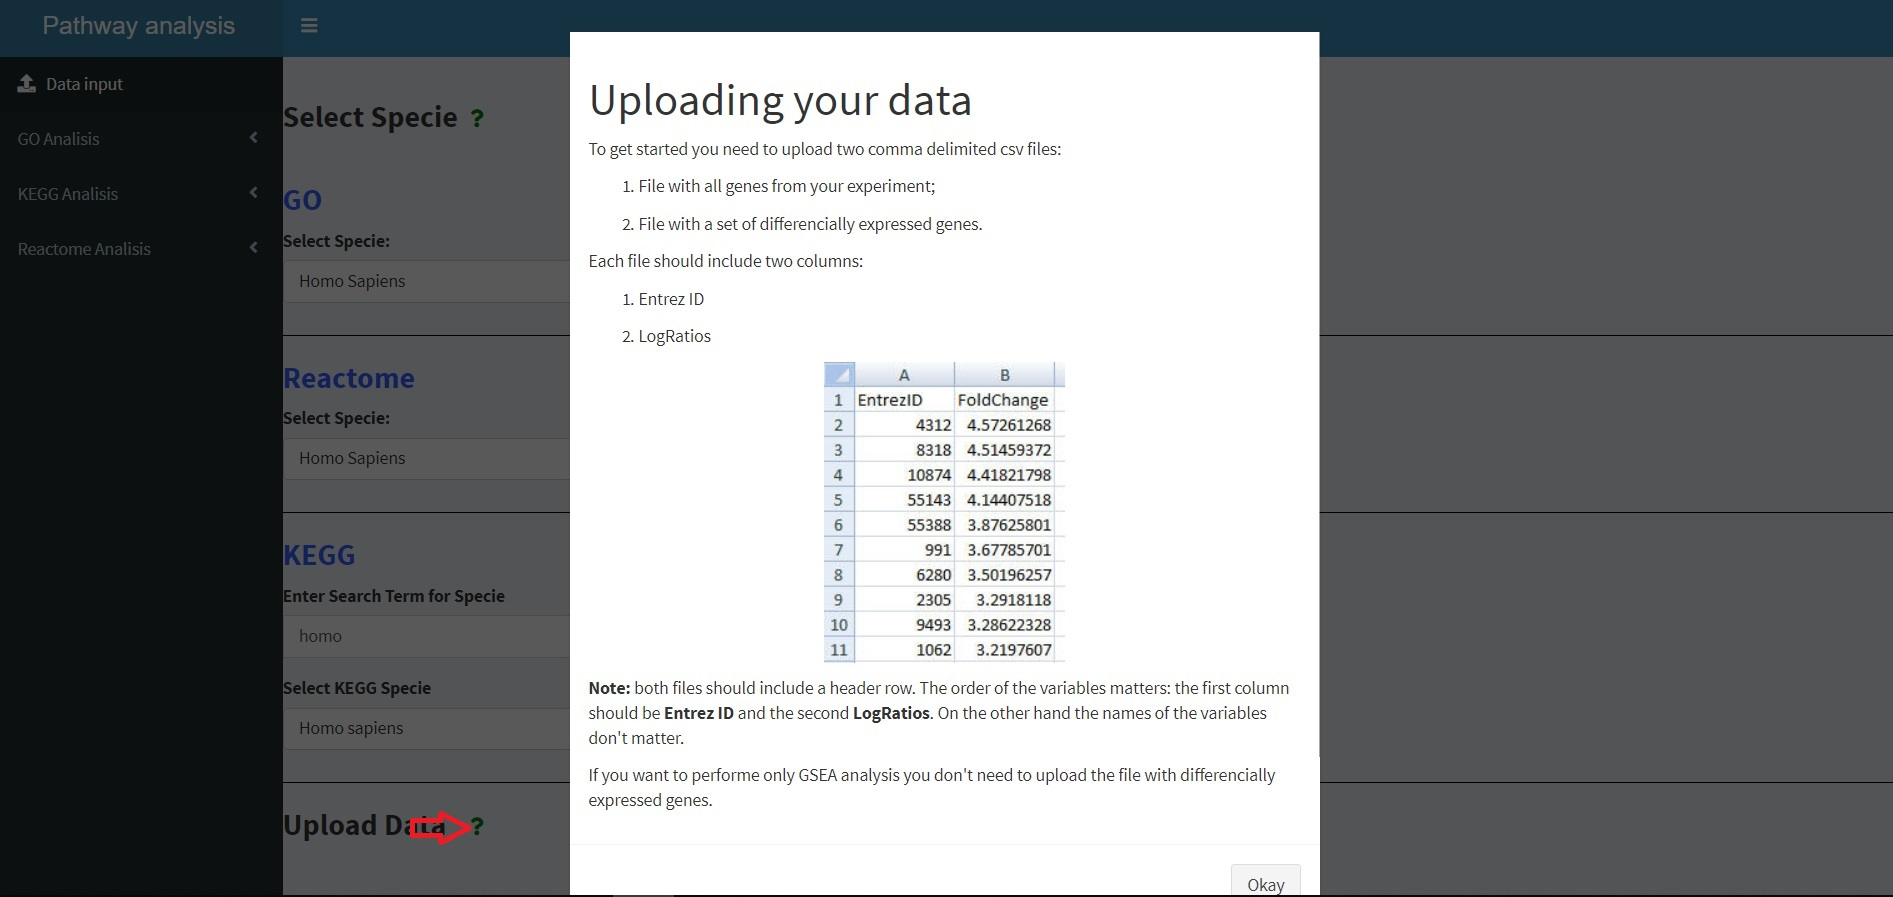
\includegraphics[width=0.9\textwidth]{figures/Help_Upload_Data.jpg} 
\caption{Ajuda per pujar les dades}
\end{figure}

Les informacions per a l'apartat \gls{ORA} són les següents:

\begin{figure}[H]
\centering
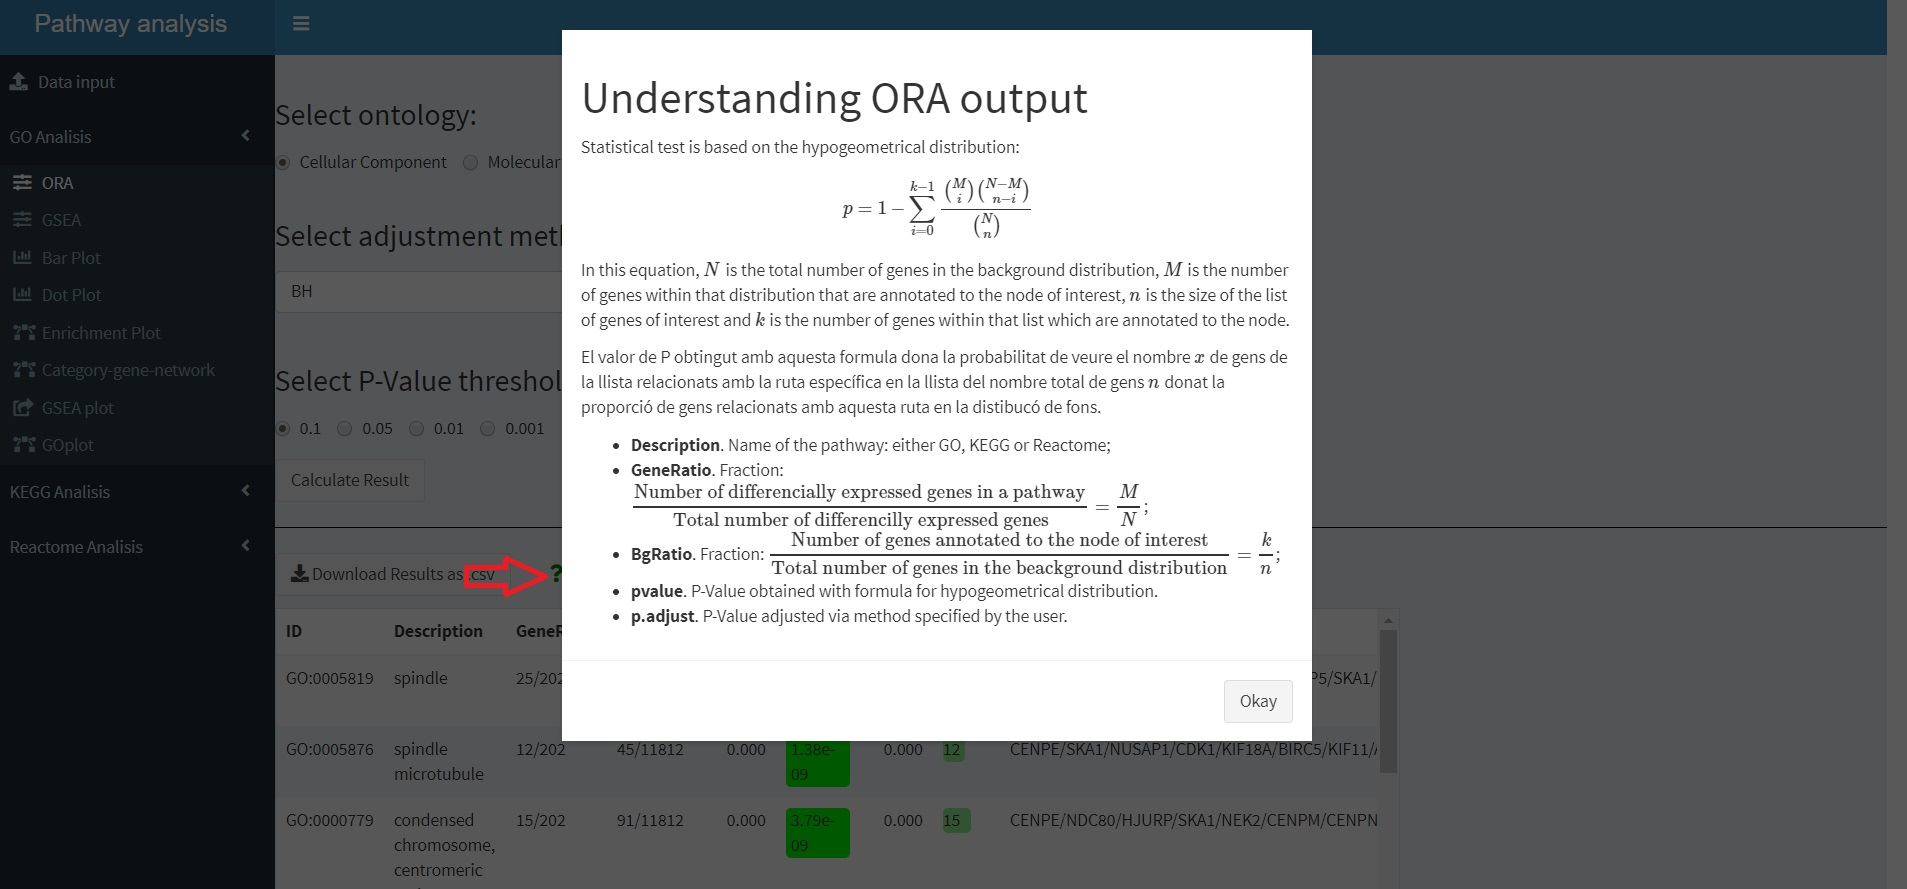
\includegraphics[width=0.9\textwidth]{figures/Help_ORA_output.jpg} 
\caption{Infromació per la interpretació d'anàlisi ORA}
\end{figure}
Aquí cal destacar que les fòrmules, depenent de l'ordinador, no apareixen degudament en el RStudio Browser. Sí que apareixen bé quan l'aplicació s'obre via l’internet browser. L'usuari ha de tenir connexió amb internet perquè l'aplicació pugui descodificar la fòrmula via MathJax. Encara no he trobat la causa per la qual el Rstudio Browser en alguns ordinadors no visualitza bé les fòrmules. Pot ser un problema amb Java, que s'ha d'actualitzar? Ho estic investigant.

\begin{figure}[H]
\centering
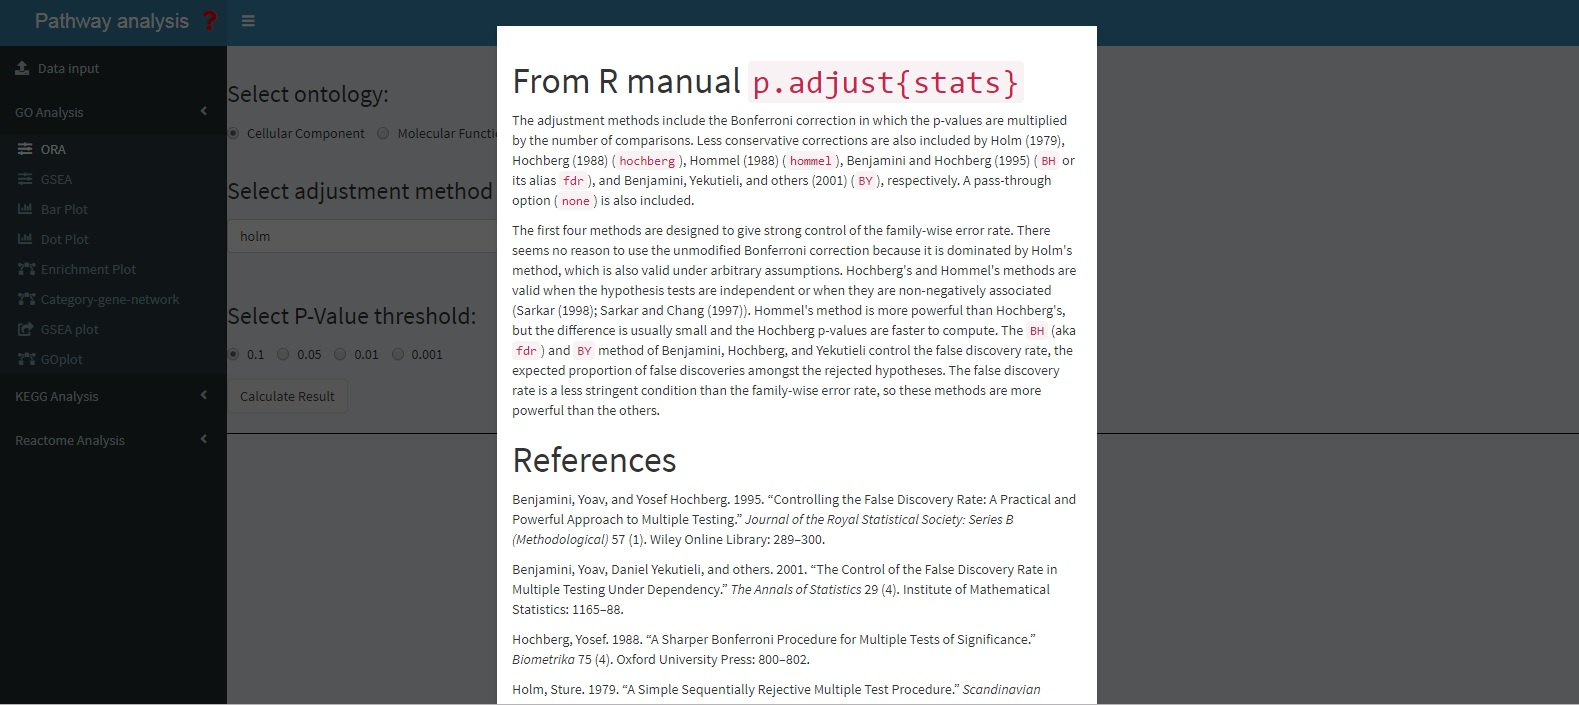
\includegraphics[width=0.9\textwidth]{figures/Help_pAdjustMethod.jpg} 
\caption{L'ajuda per a la selecció del mètode d'ajustament}
\end{figure}


\begin{figure}[H]
\centering
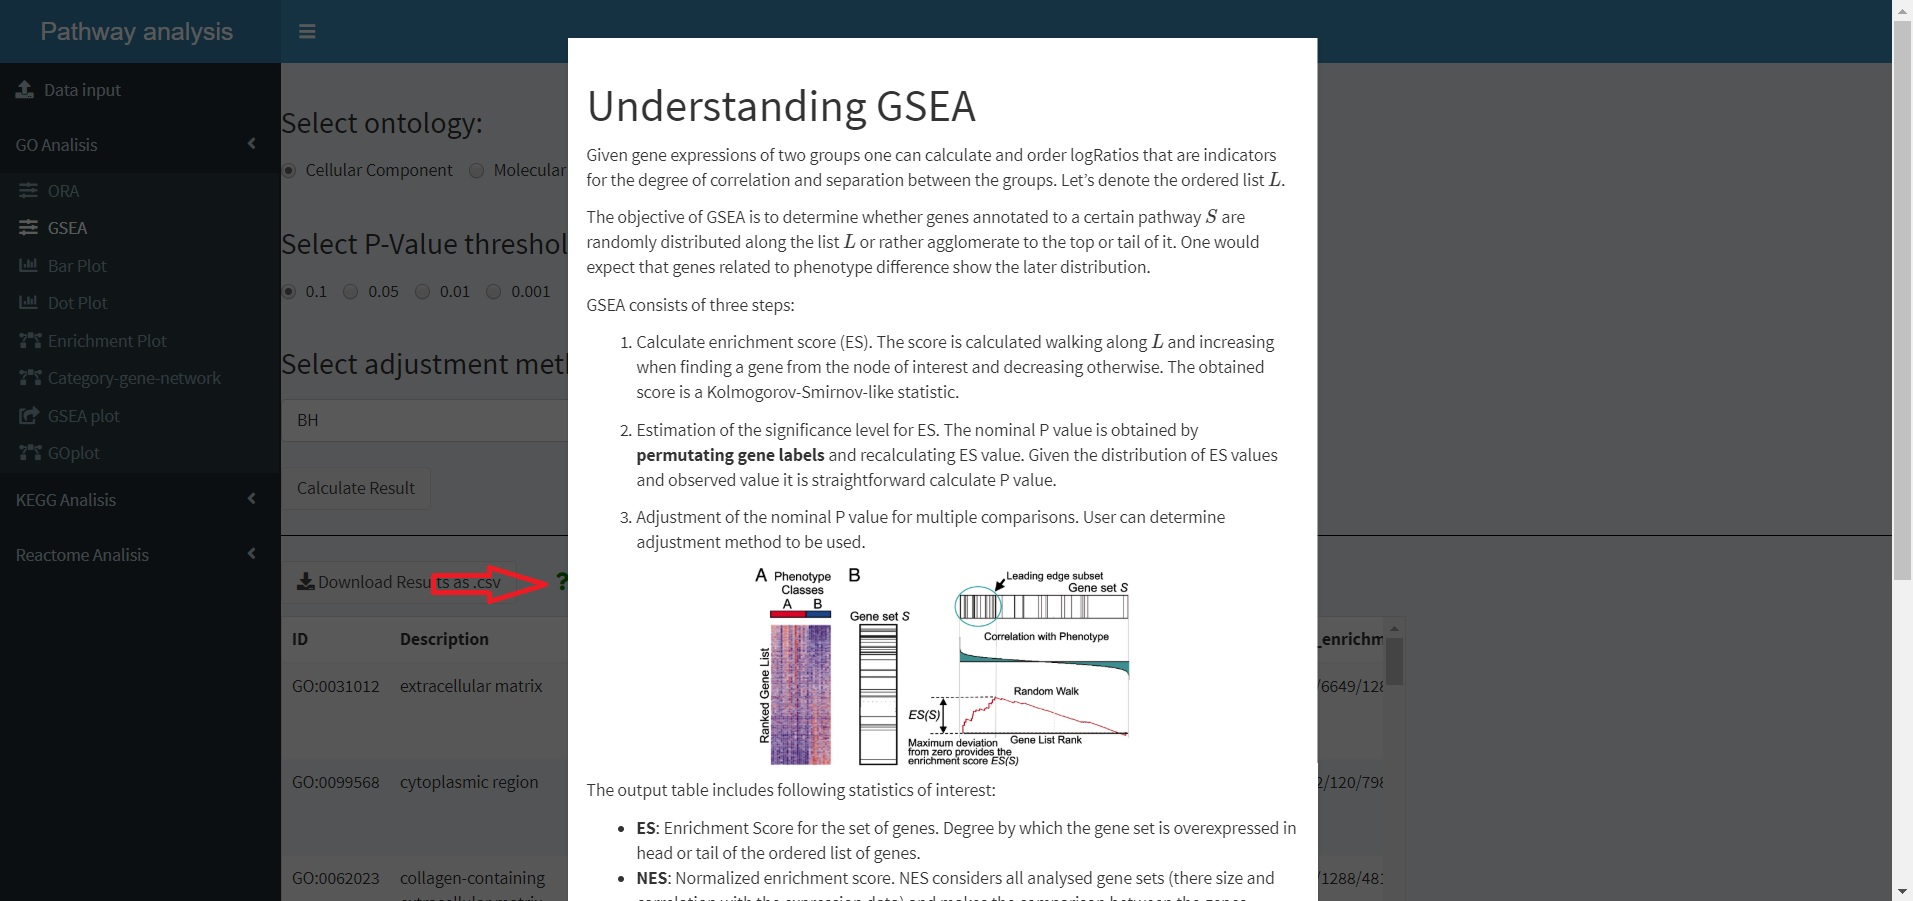
\includegraphics[width=0.9\textwidth]{figures/Help_GSEA_output.jpg} 
\caption{Ajuda per la interpretació de GSEA}
\end{figure}


\chapter{Validació dels resultats}
\label{sec:ValRes}

L’anàlisi de les rutes representa l’últim pas de l’anàlisi d’expressions. Per dur a terme l’anàlisi de rutes és necessari tenir unes dades que ja estiguin processades prèviament (normalització, càlcul de les LogRatios, ajustament dels gens repetits a l’array, selecció dels gens diferencialment expressats, etc.). Les dades de \href{https://www.ncbi.nlm.nih.gov/geo/}{GEO (Gene Expression Omnibus)} estan però disponibles com a màxim en format normalitzat. Caldria doncs fer una anàlisi per arribar a un llistat de gens diferencialment expressats amb les logRatios per tots els gens de la mostra. Fer això no seria cap problema i de fet ho he fet per altres estudis. El problema és que arribo a resultats diferents dels resultats dels estudis d’on provenen les dades. Per tant les dades que entraria a l’aplicació serien diferents de les dades de l’estudi i lògicament amb aquesta comprovació no comprovo el que realment m’interessa. He procedit a contactar el meu profesor per si tindria (o coneixeria) dades preprocessades fins a un llistat de gens amb logRatios i amb el set de gens diferencialment expressats, per tal que les pugui utilitzar en la meva aplicació. El meu professor m'ha redirigit, entre altres enllaços molt útils, al seu repositori en \href{https://github.com/alexsanchezpla?tab=repositories}{github.com}. 


\begin{table}[ht]
\centering
\begin{adjustbox}{width=1\textwidth}
\small
\begin{tabular}{||c | c | c | c | c ||} 
\hline 
Estudi & GEO ID & Espècie & Tipo d'experiment & Font \\ [0.5ex] 
\hline\hline
\cite{schmidt2008humoral} & \href{https://www.ncbi.nlm.nih.gov/geo/query/acc.cgi?acc=GSE11121}{GSE11121}& Homo sapiens & Microarrays & \href{https://bioconductor.org/packages/release/bioc/html/DOSE.html}{Paquet \helvetica{DOSE} de Bioconductor}\\
\hline
\cite{li2017zbtb7b} & \href{https://www.ncbi.nlm.nih.gov/geo/query/acc.cgi?acc=GSE100924}{GSE100924}& Mus musculus & Microarrays & \href{https://github.com/alexsanchezpla/StatisticalAnalysisOfMicroarrayData}{Github Sanchez Pla} \\ 
\hline
\cite{farmer2005identification} & \href{https://www.ncbi.nlm.nih.gov/geo/query/acc.cgi?acc=GSE1561}{GSE1561}&Homo sapiens& Microarrays & \href{https://github.com/alexsanchezpla/Ejemplo_de_MDA_con_Bioconductor}{Github Sanchez Pla} \\ 
\hline
\cite{hengel2003cutting} & \href{https://david.ncifcrf.gov/helps/demo1.txt}{DAVID Demo List 1}&Homo sapiens& Microarrays & \href{https://david.ncifcrf.gov/content.jsp?file=FAQs.html}{DAVID} \\ 
\hline
\end{tabular}
\end{adjustbox}
\end{table} 

Les dades de \cite{schmidt2008humoral}, que s'utilitzen en els vignettes de \helvetica{clusterProfiler} i \helvetica{ReactomePA}, ja les he mostrat en gran part a dalt quan explicava el contingut de l'aplicació. Els resultats obtinguts amb l'aplicació són iguals als resultats en els vignettes mencionats. Procediré doncs amb l'exemple basat en les dades de \cite{li2017zbtb7b} .

\section{Exemple d'anàlisi 1. GEO: GSE100924}

\cite{li2017zbtb7b} analitzen l'associació del gen Zbtb7b amb la produccó de les grasses marons que al seu torn influeixen termogenesis i procesos metabòlics diferents. D'aquesta manera les grasses marons són importants per a tractament dels disorders metanòlics.

Les dades d'estudi són ja preprocessades per Ricardo Gonzalo Sanz i Sanchez Pla i estan disponibles a \href{https://github.com/alexsanchezpla/StatisticalAnalysisOfMicroarrayData}{github}. De la carpeta \textit{results} he agafat la taula \textit{topAnnotated\_KOvsWT\_COLD.csv}. Sanz i Pla utilitzen el paquet \helvetica{ReactomePA} per a l'anàlisi d'enriquiment. Repeteixo doncs el seu anàlisi utilitzant l'aplicació. 


\begin{enumerate}

\item Ellegeixo l'espècie \textit{Mus musculus} per a GO, KEGG i Reactome.
\begin{figure}[H]
\centering
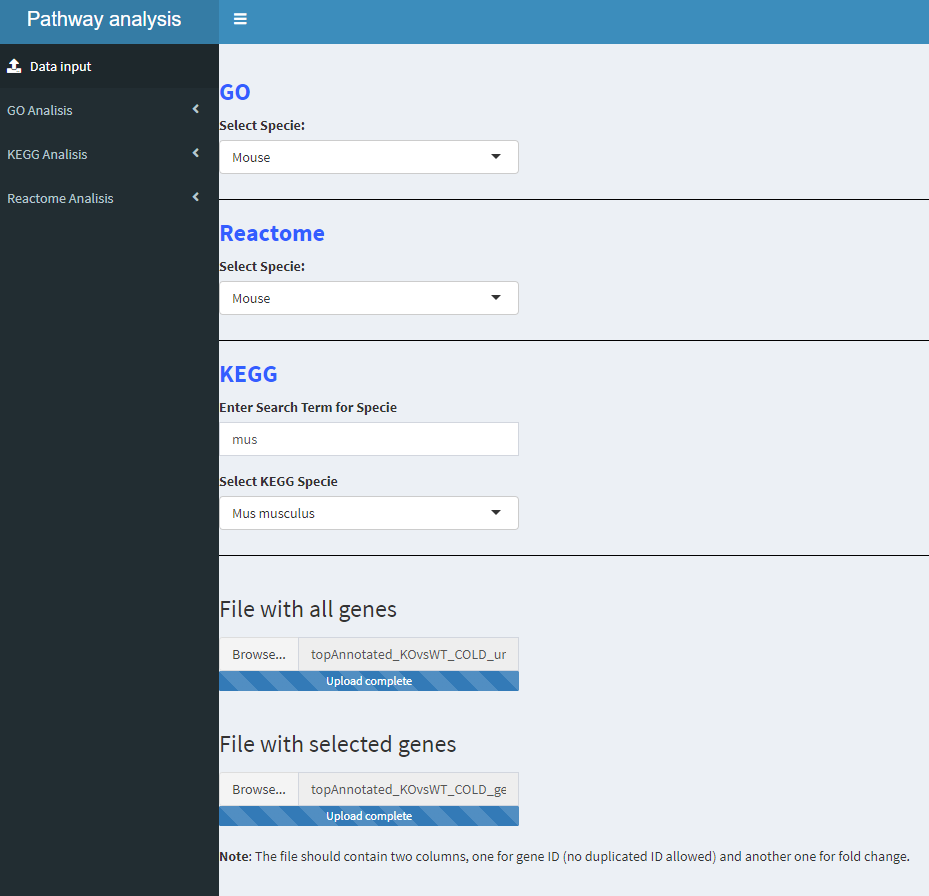
\includegraphics[width=0.6\textwidth]{figures/Estudi1_Fig1_Select_Specie.png} 
\caption{Selecció d'espècie}
\end{figure}

L'output a baix indica que s'ha pujat el total de 5995 gens. Per a l'arxiu dels gens seleccionats l'aplicació diu que s'han pujat 769 gens.

\begin{figure}[H]
\centering
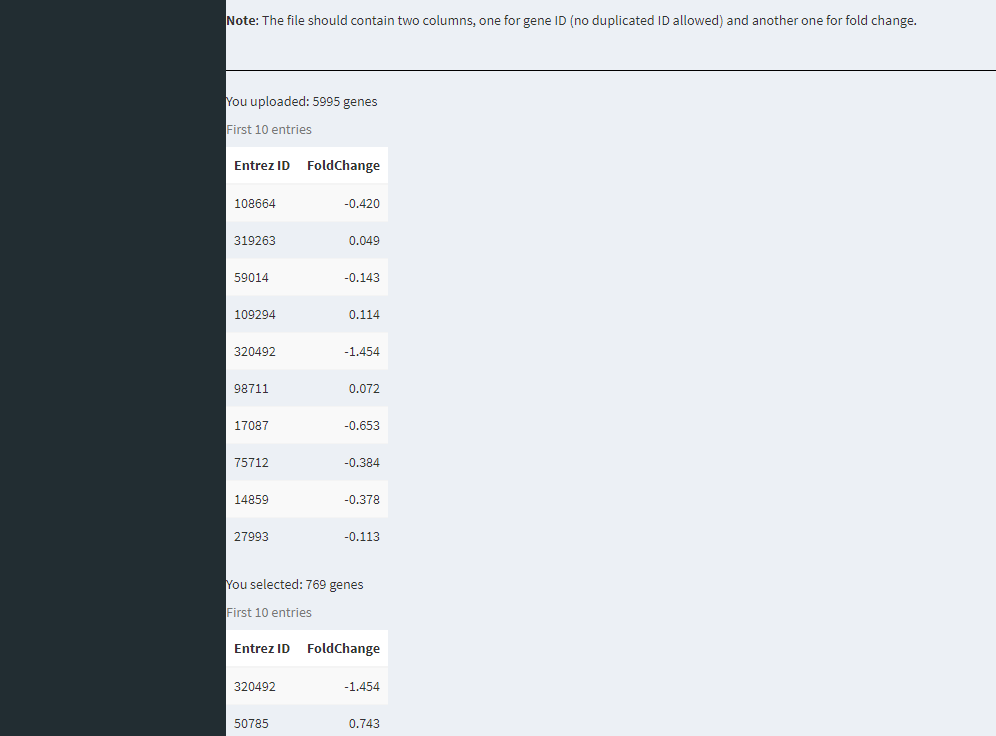
\includegraphics[width=0.6\textwidth]{figures/Estudi1_Fig2_Select_Specie.png} 
\caption{Selecció d'espècie}
\end{figure}


\item Clico en l'apartat \textit{Reactome Analysis}$\rightarrow$\textit{ORA}. Selecciono com a mètode d'ajustament \textit{BH} i el cut-off del valor de P ajustat 0.05. Clico a \textit{Calculate results}

\begin{figure}[H]
\centering
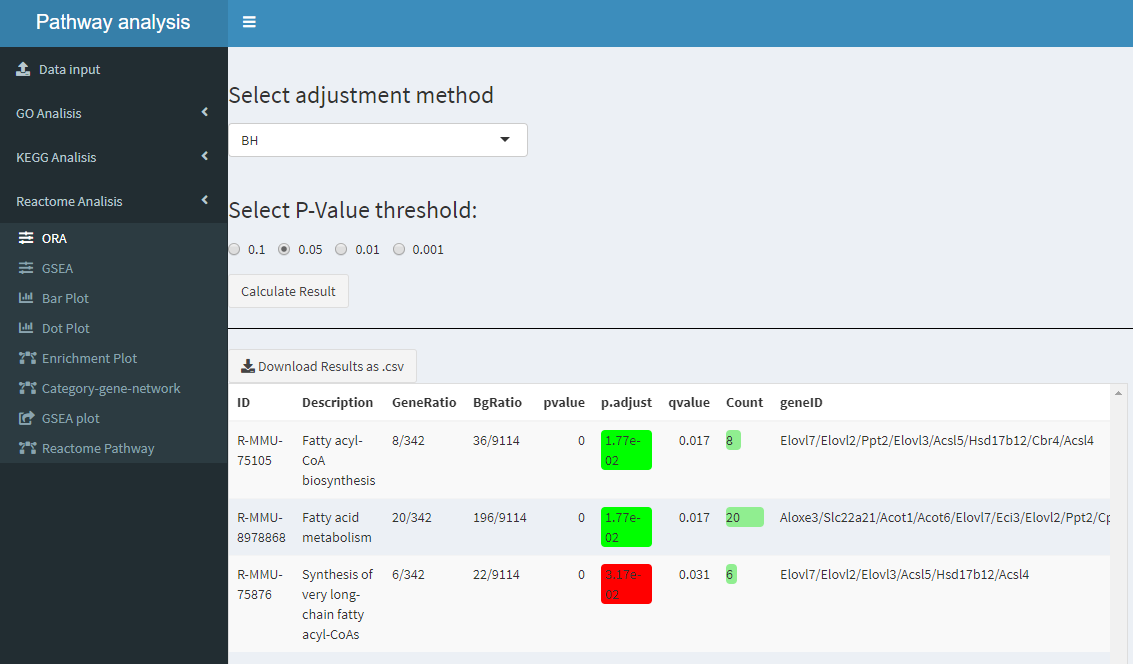
\includegraphics[width=0.6\textwidth]{figures/Estudi1_Fig3_ORA_RA.png} 
\caption{Resultat d'anàlisi \gls{ORA} de Reactome}
\end{figure}

Observem que les rutes mostrats són els mateixos esmentats per Sanz i Pla. També destaquem que el resultat conicideix amb les torbades d'estudi de \cite{li2017zbtb7b}. S'observa la perturbació de les rutes relacionades amb les grasses marrons \textbf{Fatty acyl-CoA biosynthesis} i \textbf{Fatty-acid metabolism}.

\item Visualització del resultat ORA

L'aplicació permet visualitzar els resultats obtinguts amb la ORA. 

\begin{itemize}
\item Selecciono \textit{Reactome Analysis}$\rightarrow$\textit{Bar Plot}

\begin{figure}[H]
\centering
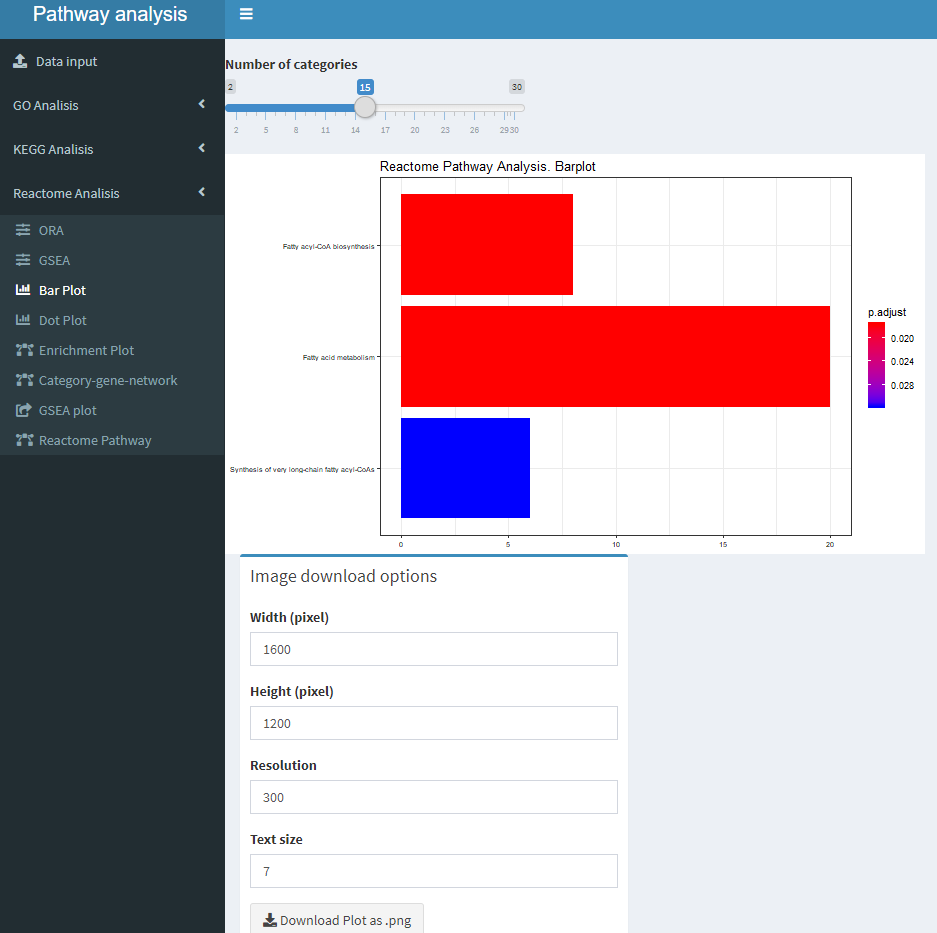
\includegraphics[width=0.6\textwidth]{figures/Estudi1_Fig4_ORA_BP_RA.png} 
\caption{Gràfic de barres}
\end{figure}

\item Selecciono \textit{Reactome Analysis}$\rightarrow$\textit{Dot Plot}

\begin{figure}[H]
\centering
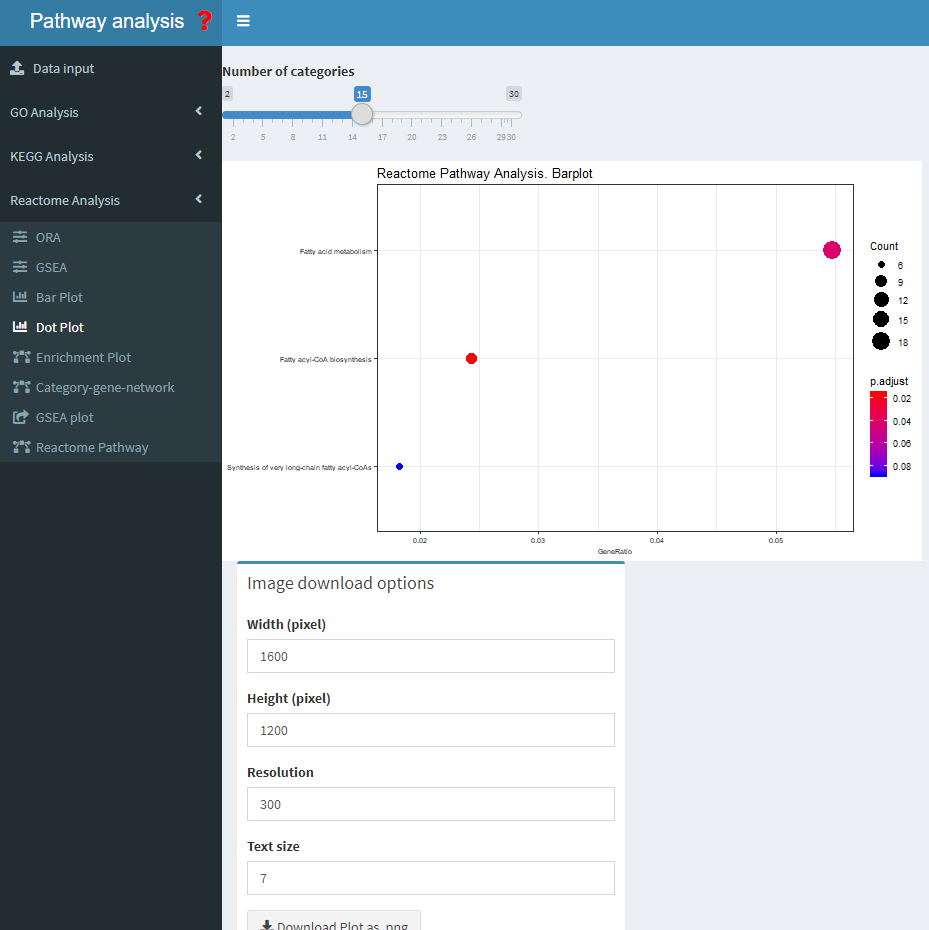
\includegraphics[width=0.6\textwidth]{figures/Estudi1_Fig5_ORA_Dot_RA.png} 
\caption{Gràfic de punts}
\end{figure}

\item Selecciono \textit{Reactome Analysis}$\rightarrow$\textit{Enrichment Map Plot}

\begin{figure}[H]
\centering
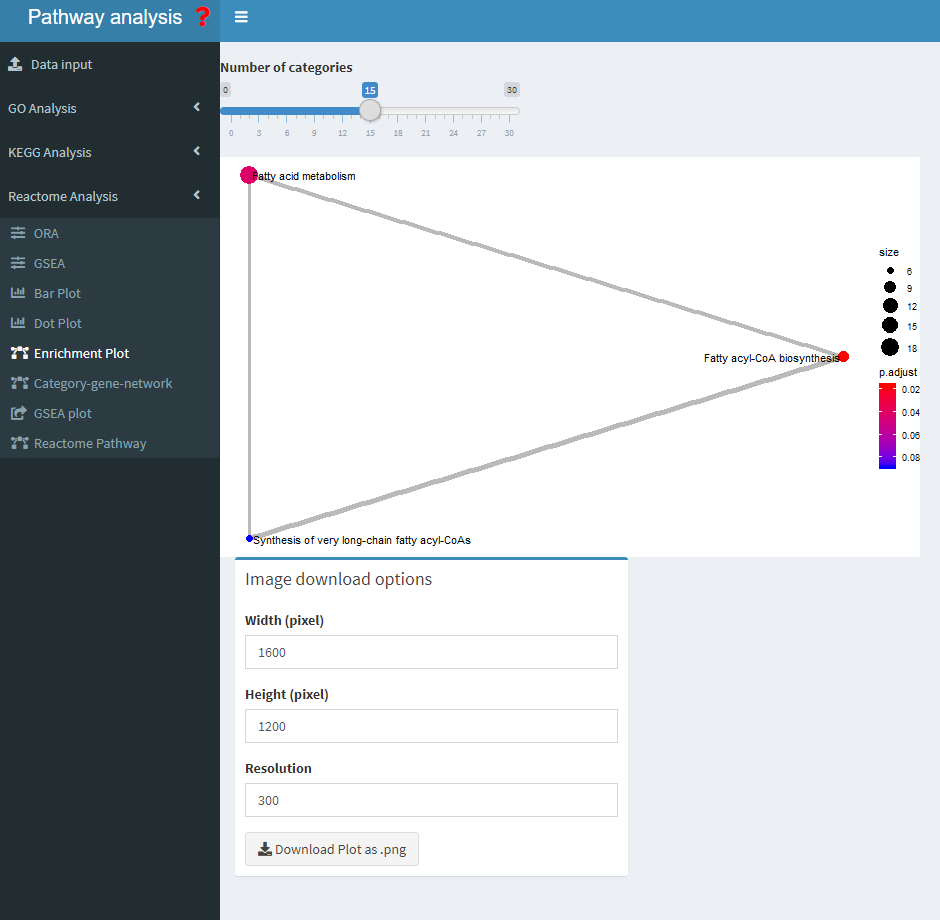
\includegraphics[width=0.6\textwidth]{figures/Estudi1_Fig6_ORA_EP_RA.png} 
\caption{Mapa d'enriquement}
\end{figure}

\item Selecciono \textit{Reactome Analysis}$\rightarrow$\textit{Category Gene Network}
Aquesta visualització incorpora les gens individuals de la ruta i el magnitud de la seva expressió diferencial. Observem que el gen Evol3 està sotaexpressat, tal com es comenta al paper de \cite{li2017zbtb7b}.

\begin{figure}[H]
\centering
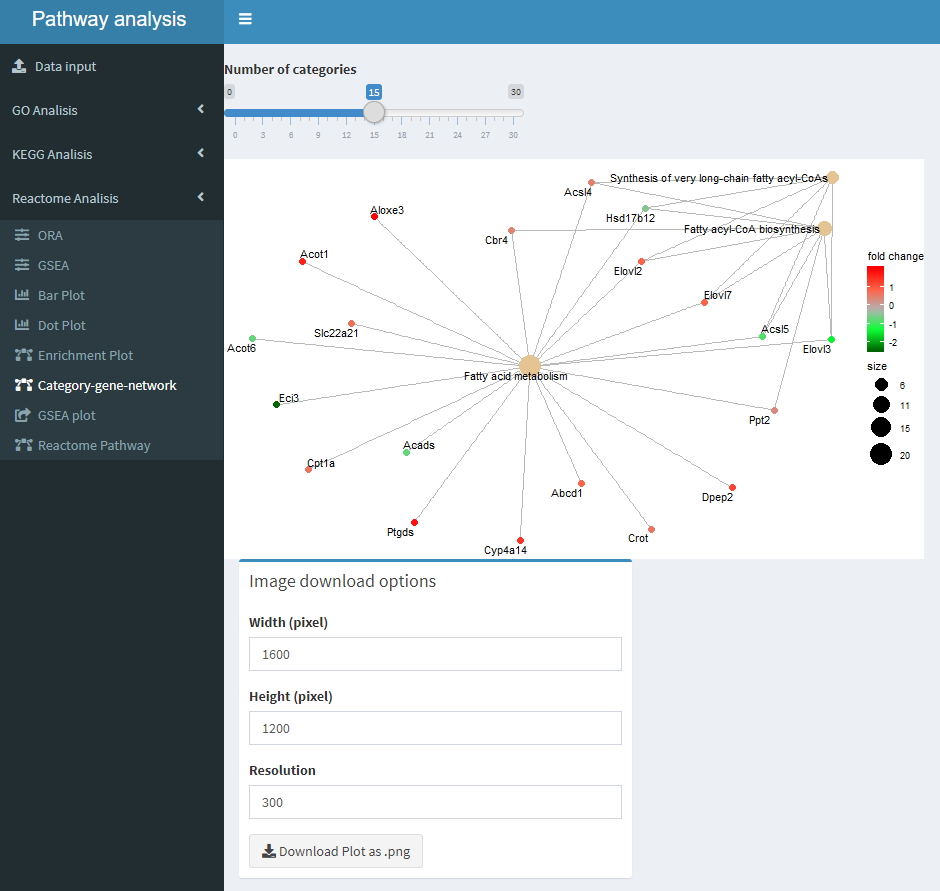
\includegraphics[width=0.6\textwidth]{figures/Estudi1_Fig7_ORA_CP_RA.png} 
\caption{Red de les categories i gens}
\end{figure}

\item Selecciono \textit{Reactome Analysis}$\rightarrow$\textit{Reactome Pathway}
\begin{figure}[H]
\centering
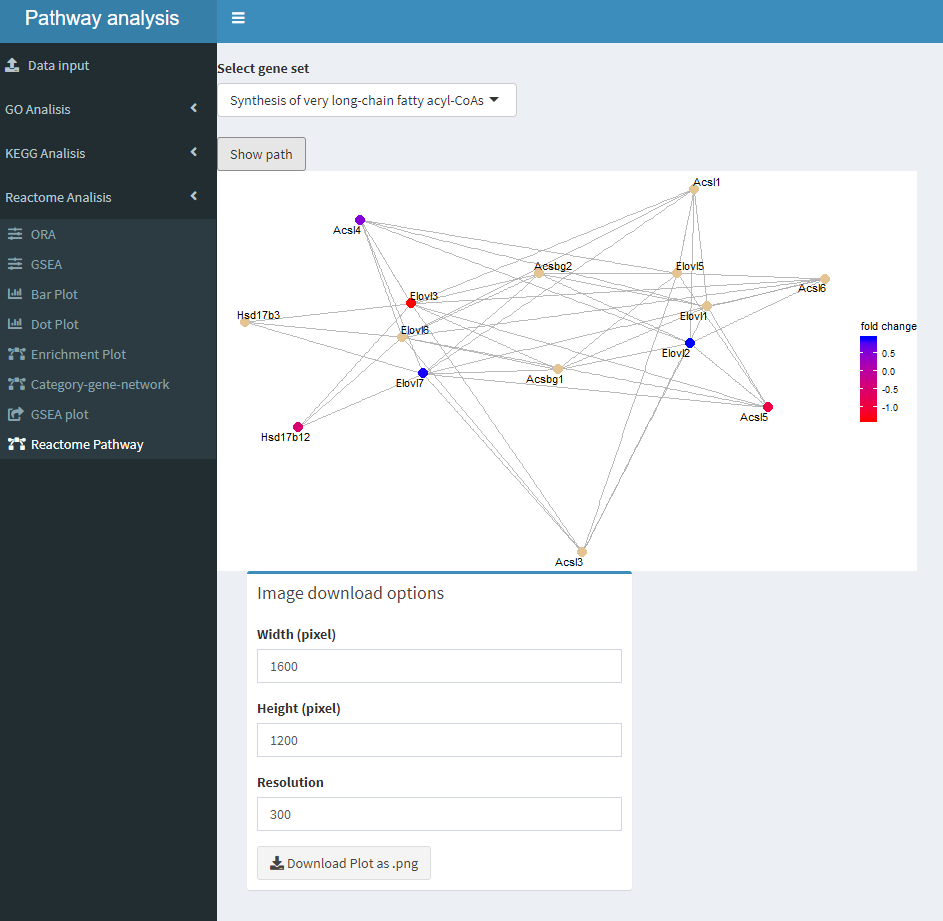
\includegraphics[width=0.6\textwidth]{figures/Estudi1_Fig8_ORA_PP_RA.png} 
\caption{Rutes Reactome}
\end{figure}
\end{itemize}
\end{enumerate}

Addicionalment a l'anàlisi \gls{ORA} podem fer, mitjançant l'aplicació, l'anàlisi GSEA per les rutes de Reactome. Per fer-ho:

\begin{enumerate}

\item Clico en l'apartat \textit{Reactome Analysis}$\rightarrow$\textit{GSEA}. Selecciono com a mètode d'ajustament \textit{BH} i el cut-off del valor de P ajustat 0.05. Clico a \textit{Calculate results}

Amb el valor de P de 0.05 l'anàlisi no troba cap ruta enriquida.

\item Augmento el Cut-Off del valor de P a 0.1

Amb el Cut-Off més alt l'aplicació retorna un llistat de gens.

\begin{figure}[H]
\centering
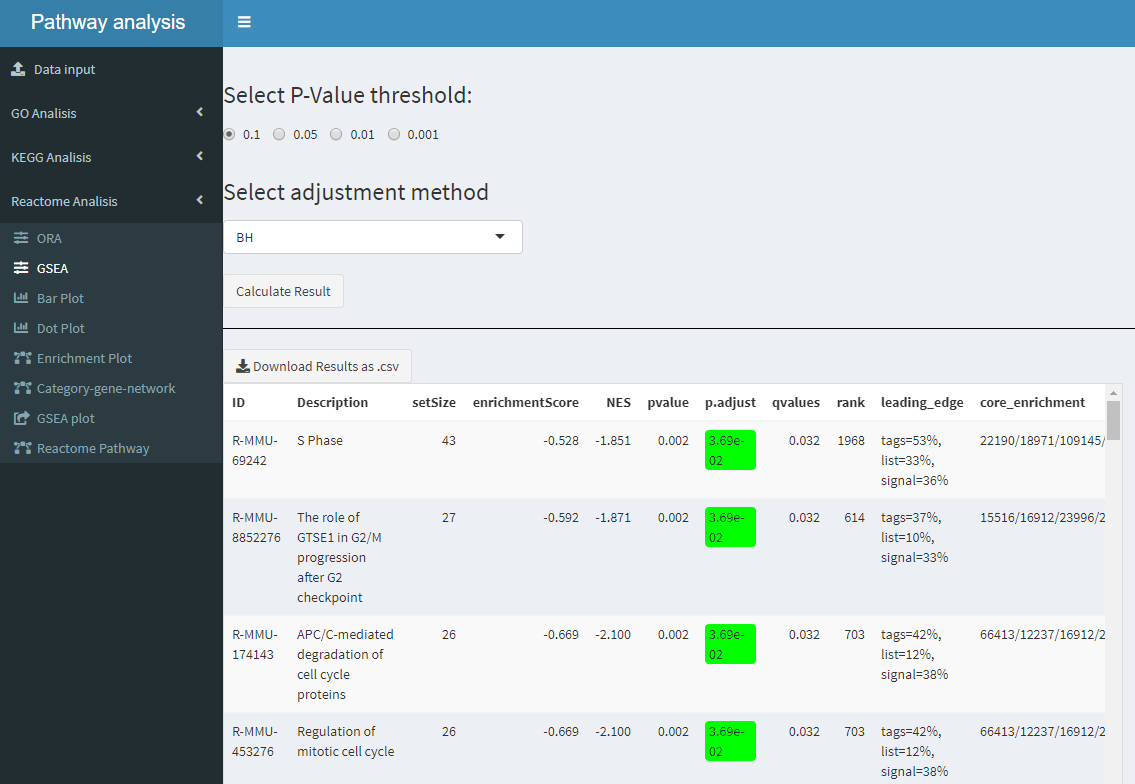
\includegraphics[width=0.6\textwidth]{figures/Estudi1_Fig9_GSEA_RA.png} 
\caption{Anàlisi GSEA}
\end{figure}

\item Per obtenir els gràfics GSEA anem a \textit{Reactome Analysis}$\rightarrow$\textit{GSEA plot}

\begin{figure}[H]
\centering
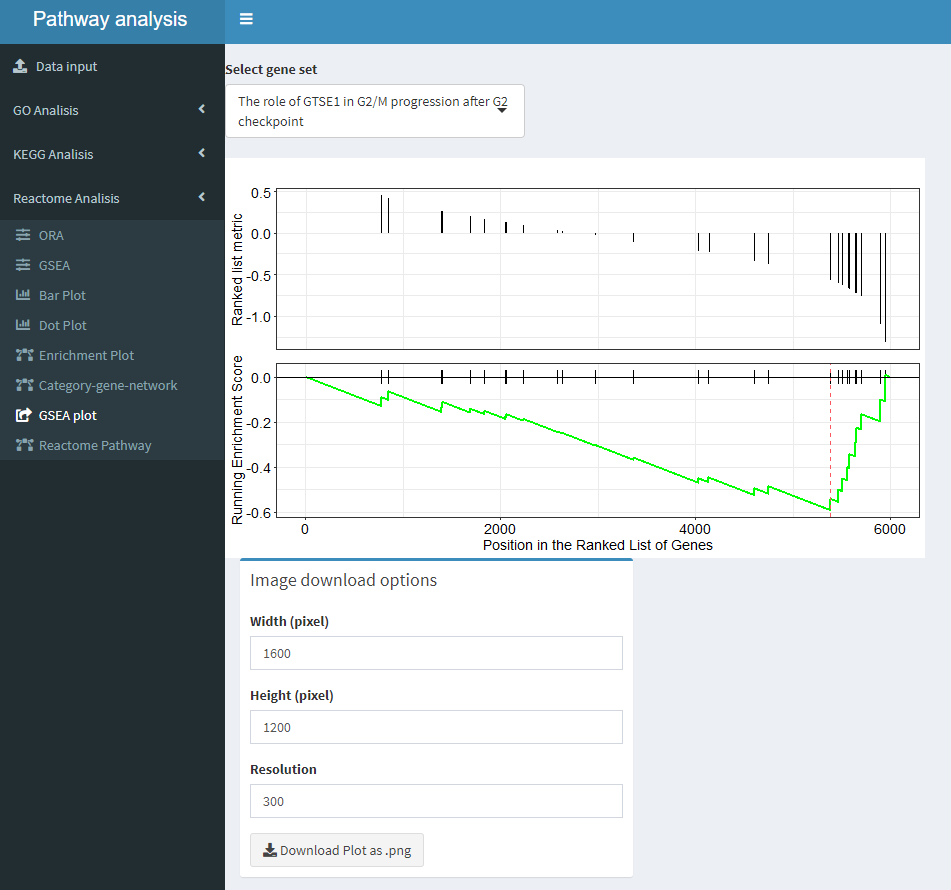
\includegraphics[width=0.6\textwidth]{figures/Estudi1_Fig10_GSEA_RA.png} 
\caption{Gràfic GSEA}
\end{figure}
\end{enumerate}

També podem fer l'anàlisi de KEGG. El resultat de KEGG és similar a l'anàlisi de Reactome. L'aplicació permet però generar les rutes KEGG. Per obtenir-les:

\begin{enumerate}
\item Clico en l'apartat \textit{KEGG Analysis}$\rightarrow$\textit{ORA}. Selecciono com a mètode d'ajustament \textit{BH} i el cut-off del valor de P ajustat 0.05. Clico a \textit{Calculate results}
\begin{figure}[H]
\centering
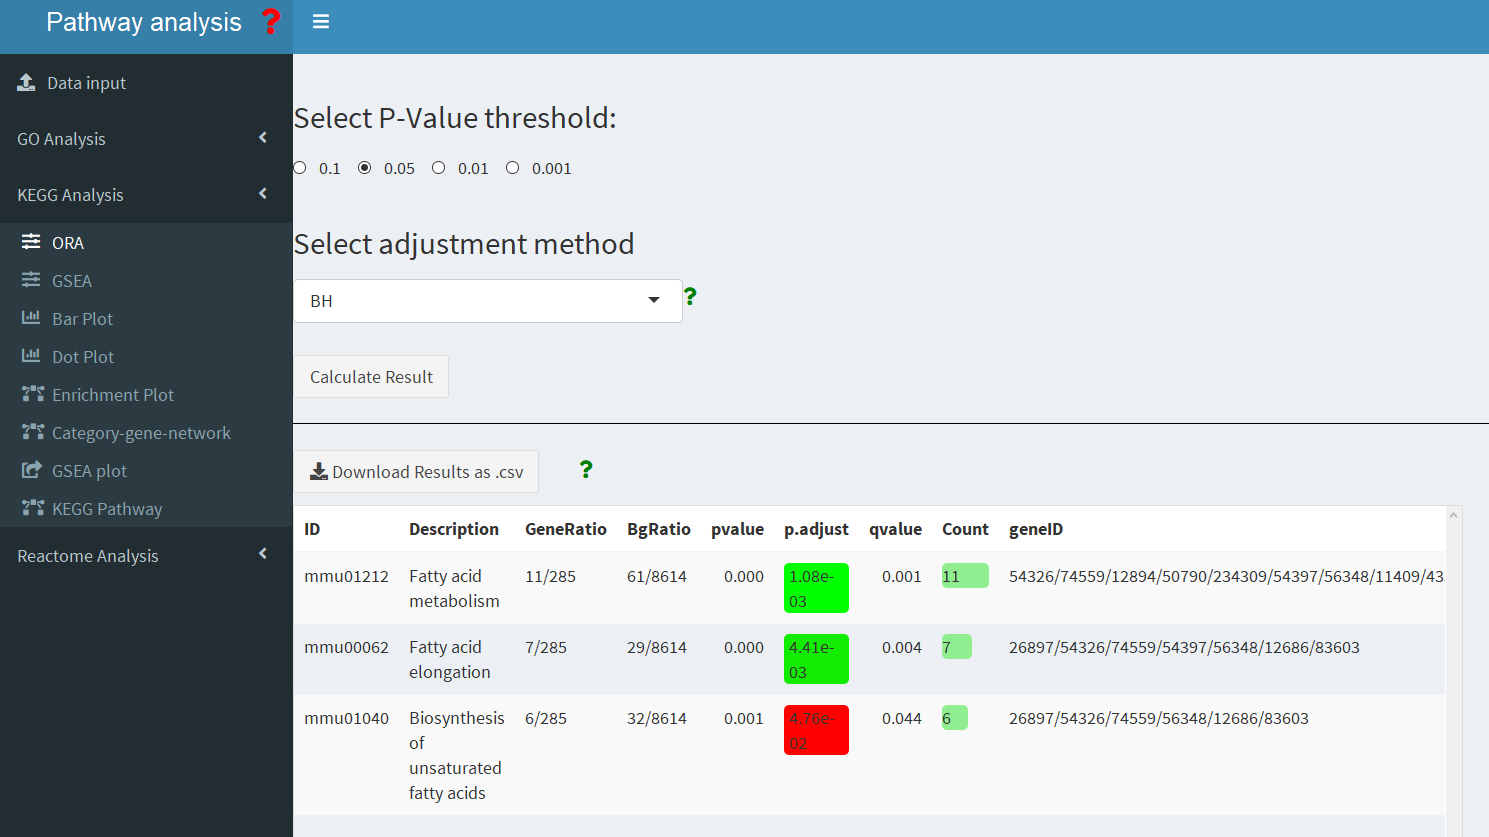
\includegraphics[width=0.6\textwidth]{figures/Estudi1_Fig11_ORA_KEGG.png} 
\caption{Anàlisi \gls{ORA} de KEGG}
\end{figure}

\item Anem a \textit{KEGG}$\rightarrow$\textit{KEGG Pathway}
\begin{figure}[H]
\centering
\includegraphics[width=0.6\textwidth]{figures/Estudi1_Fig12_KEGG_Pathway.png} 
\caption{Gràfic de les rutes KEGG}
\end{figure}
\end{enumerate}

L'anàlisi GO no retorna cap terme GO amb el nivell de significació de 0.05. Pujant el nivell de significació fins 0.1 retorna un llistat dels termes enriquits per als components cel·lulars.

Clico en l'apartat \textit{GO Analysis}$\rightarrow$\textit{ORA}. Selecciono com a mètode d'ajustament \textit{BH} i el cut-off del valor de P ajustat 0.1. Selecciono també \textit{CC}. Clico a \textit{Calculate results}
\begin{figure}[H]
\centering
\includegraphics[width=0.6\textwidth]{figures/Estudi1_Fig13_GO.png} 
\caption{L'anàlisi \gls{ORA} de GO}
\end{figure}

\chapter{Conclusió}

Al treball final he tingut com a objectiu la creació d'una aplicació per a anàlisi de les rutes. Primer he determinat que és l'anàlisi de les rutes i on es situa a l'anàlisi global d'expressió genètica. He explicat que l'anàlisi de les rutes és l'ultim pas de l'anàlisi d'expressió gènica on es preten fer sentit biològic de les dades d'expressió. Per dur a terme aquest anàlisi s'utilitza una llista dels gens diferencialment expressats i els logRatios de tots els gens d'experiment. He explicat que es necessari anotar aquests gens a les bases existents per poder agrupar-los als conceptes (o rutes). He triat les bases de dades més coneguts i que són utilitzades pels paquets de Bioconductor. Aquestes bases de dades són: GO (Gene Ontology), KEGG (Kyoto Encyclopedia of Genes  and Genomes) i Reactome. He descrit quins mètodes existen per calcular la significació biològica de les rutes. Entre altres he identificat tres estratègies:  \gls{ORA} (Over-Representation Analisis), FCS (Functional Class Scoring) i l'anàlisi topològic de les rutes. He desctit amb més detall les mètodes \gls{ORA} i GSEA i també he identificat les possibilitats per visualitzar les rutes.  Després de formular un protocol d'anàlisi he buscat i identificat els paquets de Bioconductor que permiten aplicar els mètodes descrits. Entre altres he triat \helvetica{clusterProfiler}, \helvetica{ReactomePA} i \helvetica{pathview}. He posat aquests paquets com a base per la futura aplicació. El resultat era l'aplicació dividida en quatre apartats: 1) Entrada de les dades; 2) Anàlisi amb la base d'anotació GO; 3) L'anàlisi amb la base d'anotació KEGG i l'anàlisi amb la base d'anotació Reactome. Per a cada base de dades l'usuari pot fer ORA, GSEA i obtenir visualització de la topologia de les rutes. L'aplicació perment descargar els resultats com a l'arxiu .csv i imatges .png, les quals l'usuari pot personalitzar. La validació dels resultats ha mostrat una bona coincidència amb l'estudi triat per validar les dades.  Aquest estudi investiga l'impacte del gen Zbtb7b sobre la producció de les grasses marrons. Justament les rutes relacionades amb el síntesi de grasses marrons estaben identificats amb l'aplicació. L'aplicació pot ser descargada i instal·lada llibrement del repositori GitHub i la via per fer-ho s'explica a la memòria. Actualment es busca el mètode per publicar l'aplicació a l'internet per fer-la encara més accessible.
 

   %% remove this line to get rid of the style chapter

%% include tex file chapters:
% \include{introduction}        %% this is a suggestion: you have to create this file on demand
% \include{problem}             %% this is a suggestion: you have to create this file on demand
% \include{solution}            %% this is a suggestion: you have to create this file on demand
% \include{evaluation}          %% this is a suggestion: you have to create this file on demand
% \include{outlook}             %% this is a suggestion: you have to create this file on demand

%\appendix                       %% closes main document, appendix follows until end; only available in book-classes
%\addpart*{Appendix}             %% adding Appendix to tableofcontents


  

\bibliography{references}
\bibliographystyle{apalike}

% \include{further_ressources}  %% this is a suggestion: you have to create this file on demand




\clearpage 
\printnoidxglossaries


%%%% end{document}
\end{document}
%% vim:foldmethod=expr
%% vim:fde=getline(v\:lnum)=~'^%%%%\ .\\+'?'>1'\:'='
%%% Local Variables:
%%% mode: latex
%%% mode: auto-fill
%%% mode: flyspell
%%% eval: (ispell-change-dictionary "en_US")
%%% TeX-master: "main"
%%% End:
